\documentclass[10pt]{amsbook}

% \usepackage{graphicx}
\usepackage{chemarr}
\usepackage{amsfonts}
\usepackage{amssymb}
\usepackage{amsmath}
\usepackage{latexsym}
\usepackage{epsfig}
\usepackage{amsthm}
\usepackage[Lenny]{fncychap}
\usepackage{hyperref}

\renewcommand{\chaptermark}[1]{%
\markboth{\chaptername
\ \thechapter.\ #1}{}}

\usepackage{lipsum} % for filler text
\usepackage{fancyhdr}
\pagestyle{fancy}
\fancyhead{} % clear all header fields
\fancyhead[RE,LO]{\small\textsf{\rightmark}}
\fancyhead[RO,LE]{\small\textsf{\thepage}}
\renewcommand{\headrulewidth}{0pt} % no line in header area
\fancyfoot{} % clear all footer fields
\fancyfoot[C]{\small\textsf{Eric Klavins: A Systems Approach to Synthetic Biology}} % other info in "inner" position of footer line

 \usepackage[small]{caption}

%
% From: http://www.ams.org/authors/monopackages.html
%
\newtheorem{theorem}{Theorem}[chapter]
\newtheorem{lemma}[theorem]{Lemma}
\newtheorem{property}[theorem]{Property}

\theoremstyle{definition}
\newtheorem{definition}[theorem]{Definition}

\theoremstyle{definition}
\newtheorem{example}[theorem]{Example}

\newtheoremstyle{exercise}% name
     {3pt}%      Space above
     {6pt}%      Space below
     {}%         Body font
     {}%         Indent amount (empty = no indent, \parindent = para indent)
     {}% Thm head font
     {)}%        Punctuation after thm head
     {.5em}%     Space after thm head: " " = normal interword space;
           %       \newline = linebreak
     {}

\newcounter{exercount}
\theoremstyle{exercise}
\newtheorem{exercise}[exercount]{}
\renewcommand{\theexercount}{\thechapter.\arabic{exercount}}

\theoremstyle{remark}
\newtheorem{remark}[theorem]{Remark}

\numberwithin{section}{chapter}
\numberwithin{equation}{chapter}

\makeatletter
\renewcommand\paragraph{%
   \@startsection{paragraph}{4}{0mm}%
      {-\baselineskip}%
      {-\baselineskip}%
      {\normalfont\normalsize\bfseries}}
\makeatother

\newcommand{\eref}[1]{(\ref{#1})}      % FOR EQUATION REFERENCES
\newcommand{\defeq}{\triangleq}        % DEFINED TO BE EQUAL TO
\newcommand{\nats}{\mathbb{N}}
\newcommand{\positives}{\mathbb{P}}
\newcommand{\reals}{\mathbb{R}}
\newcommand{\ints}{\mathbb{Z}}
\newcommand{\rats}{\mathbb{Q}}
\newcommand{\complexes}{\mathbb{C}}
\newcommand{\vvec}[2]{ \left ( \begin{array}{c} #1 \\ #2 \end{array} \right ) }
\newcommand{\vvvec}[3]{ \left ( \begin{array}{c} #1 \\ #2 \\ #3 \end{array} \right ) }

\newcommand{\pd}[2]{\frac{\partial #1}{\partial #2}}

\newcommand{\enx}{ % TO END EXAMPLES
  \hfill 
  {\small $\blacktriangle$}
  \bigskip
}

\newcommand{\ev}[1]{\langle #1 \rangle}

\newcommand{\react}[1]{\xrightharpoon[]{#1}}

\newcommand{\rreact}[2]{\xrightleftharpoons[#2]{#1}}

\makeatletter
\newcommand{\xrightharpoon}[2][]{%
  \ensuremath{%
    \mathrel{%
      \settoheight{\dimen@}{\raise 2pt\hbox{$\rightharpoonup$}}%
      \setlength{\dimen@}{-\dimen@}%
      \edef\CA@temp{\the\dimen@}%
      \settoheight\dimen@{$\rightleftharpoons$}%
      \addtolength{\dimen@}{\CA@temp}%
      \raisebox{\dimen@}{%
        \rlap{%
          \raisebox{2pt}{%
            $%
            \ext@arrow 0359\rightharpoonupfill@{\hphantom{#1}}{#2}%
            $%
          }%
        }%
        \hbox{%
          \raisebox{2pt}{%
            $%
            \ext@arrow 0359\rightharpoonupfill@{\hphantom{#1}}{#2}%
            $%
          }%
        }%
      }%
    }%
  }%
}
\makeatother

\begin{document}

%
% Title
%
\frontmatter

\pdfbookmark[0]{Front Matter}{front}
\begin{titlepage}
\begin{center}

\vspace{1in}

{\Huge\textsf{BioCircuits:\\
\vspace{0.25in}
A Systems Approach to Synthetic Biology}}

\vspace{1in}

\textsc{Eric Klavins}

\vspace{0.25in}

\textsc{Department of Electrical Engineering\\
University of Washington\\
Seattle, WA}

\vfill
 
% Bottom of the page
Last compiled {\large \today}

\end{center}
\end{titlepage}

\setcounter{page}{4}

\tableofcontents

\mainmatter
\chapter{Introduction}

\section{What is Synthetic Biology?}

% life and parts description

Synthetic biology is the design and study of artificial living
organisms, re-engineered organisms, and engineered parts for existing
organisms. The idea is to bring engineering tools and methodologies to
the subject of biology, much as electrical engineering brings these
tools to physics, with the goal of designing novel and useful
biological systems. These novel systems, new life forms really, may
someday afford humanity a new level control over the processes in our
bodies, in our crops, in landfills, compost heaps, and the ocean
waters: Instead of controlling the living world with machines and
harsh chemicals, synthetic biology promises control at the level of
individual molecules using engineered living cells as tiny chemical
processing plants.

Of course, biology is more than just chemical processing. It is
information processing. The instructions for how to grow and regulate
a human being are encoded by the DNA inside each of the cells in your
body. Growth and development follows precise, distributed, robust
algorithms. The immune system can adapt itself to pathogens it has
never seen. A predator can track its prey and outsmart it. Our brains
can do research and write books. Life {\em is} computation. The
molecules and structures inside cells are the tools that nature uses
to implement life's computations, just as the silicon and wires inside
your computer implement computations. Thus, to some
extent, biology (synthetic or otherwise) ought to be seen more
abstractly than our high-school biology books would have us see
it. Our job as living system engineers is to define the abstractions,
the composable modules, the signal carriers, the simplifications, the
programming languages, and the debugging tools for living systems.

We are far from being able to engineer entirely new life forms,
although remarkable advances are being made every day. Many of these
advances are technological, such as rebooting cells so that they
become stem cells \cite{reprogramming}, putting the genome of one cell
into another \cite{cloning}, synthesizing large pieces of DNA
\cite{m-genetalium}, and improved methods for tracking molecules
inside cells \cite{fret-in-cells}. Other advances are more conceptual,
such as new understandings of stochastic chemical kinetics
\cite{khammash-fsp,el-samad-stochastic}, system identification feedback
control inside cells \cite{avano-osmotic}, directed evolution
\cite{alon}, and so on. Perhaps most telling, some advances look like
hacking: artificial oscillators inside cells
\cite{elowitz-repressilator}, engineered cell-cell communication
\cite{weiss-communicate}, digital logic inside cells
\cite{weiss-logic}. The fact that researchers in well-equipped labs
and others in their garages \cite{diy} can now make their own widgets
for living systems suggests that the technologies for and the
conceptual understandings of living systems are now sufficiently rich
to allow engineers to to tinker. And tinkering leads to engineering
research, which leads to engineering practice.

% practical description: sensing, control, actuation, information, evolution
It is fun to argue about what life {\em is} or what it would mean to
actually have built a living organism or enough of one to call it a
truely new species. However, in this book we will take a more
pragmatic approach and look, instead, at what living systems seem to
know how to do well: sense, actuate, control, process information, and
evolve. These five capabilities -- present in all the living systems
we can think of -- are probably necessary for all life forms, and in
this book we focus mainly on them as goals for what to
build. Furthermore, these capabilities, except for the last one, are
usually thought of by engineers as the important aspects of embedded
control systems (such as automobiles or cell phones). We hope to use
our experience engineering embedded systems for engineering living
systems, an idea that leads to the question: What do we mean by
sensing, actuation, control, and information processing in the context
of living systems?

%
% Should there be a formal definition of a sensor?
%  
\paragraph{Sensing:} A cell can sense all sorts of quantities, inside
itself and outside. For example, the bacterium {\em E. coli} makes a
protein called {\em LacI} (for {\em lactose inhibitor}) that changes
shape in the presence of the sugar lactose. This has downstream
effects that change the cell's metabolic machinery so that it can
efficiently digest lactose \cite{lac-operon}. Essentially, {\em LacI}
{\em senses} the presence of lactose. In fact, all cells have
molecular mechanisms that can sense the small molecules normally found
in nature, as well they should. Some of these molecules are nutrients,
some are toxins, some represent signals from other cells, and so
on. Any organism that has a good estimate of what is happening in its
environment has an advantage over less ``aware'' organisms. There are
also cells that can sense temperature \cite{heat-shock}, acidity
\cite{ph-sensor}, light \cite{light-sensor}, magnetic fields
\cite{magnetosome}, and on and on. Synthetic biologists use these
capabilities, often by putting the gene for a type of sensor found in
one organism into a genetic regulator circuit being engineered in
another, thereby giving their system new capabilities. For example,
synthetic biologists have put arsenic sensors in {\em E. coli} to make
a device that can warn users of tainted water \cite{arsenic-sensor}.

%
% NOTE: using polaroid distance sensors in robots
%

%
% Should there be a definition of an actuator?
%
\paragraph{Actuation:} A cell can alter its environment, or itself, in
a variety of ways. It can emit a small molecule as a signal to other
cells. Many cells, such as {\em E. coli}, can move by swirling their
flagella while other cells, such as amoebae, move by growing and
digesting their cytoskeletons. Internally, cells can synthesize a wide
variety of molecules that can have huge effects on the cell and its
environment. In fact, {\em making something} is a form of actuation. A
newly synthesized molecule, such as a protein, can effect structure,
metabolism, signaling within and outside of the cell, and so on. Once
again, synthetic biologists borrow the actuators from other organisms
(or make their own) and hook them up to sensors in novel ways to
create new behaviors. For example, a widely used actuator is {\em
  green fluorescent protein} (GFP) \cite{gfp}, which is a molecule
usually found in jellyfish that happens to fluoresce. Synthetic
biologists use GFP like embedded systems engineers use light emitting
diodes, as indicators that something has changed inside the cell. For
example, the arsenic sensor mentioned above is coupled to GFP
production so that cells that detect arsenic glow green under
ultraviolet (dark) light.

\begin{figure}
\centering
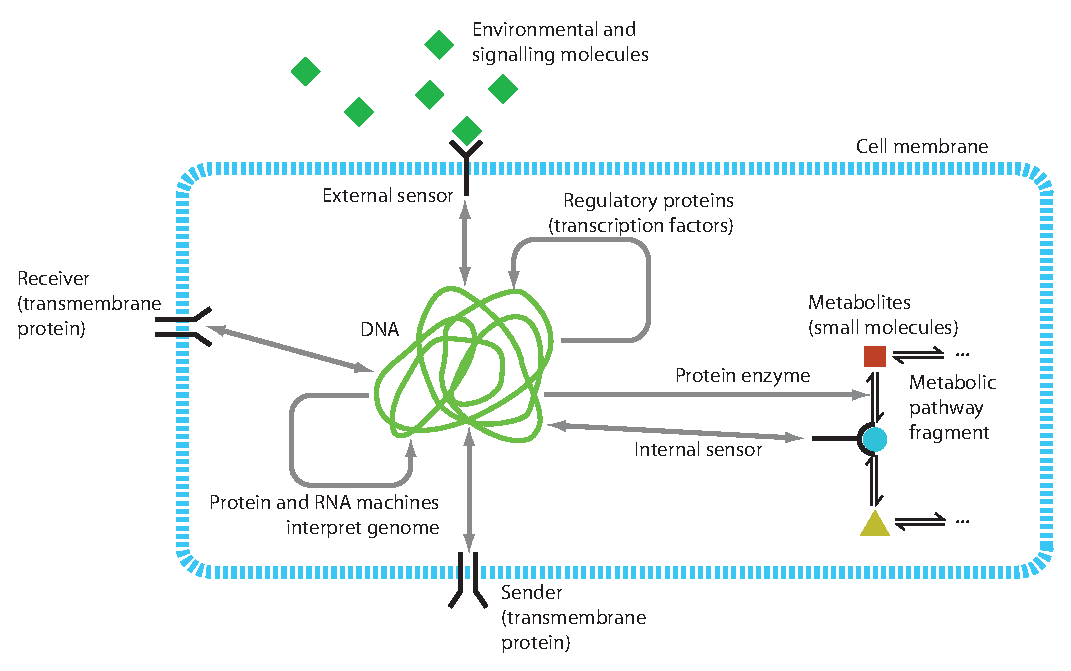
\epsfig{file=figures/cell.eps, scale=0.7}
\caption{\label{fig:thecell} The general structure of a sensing,
  control, actuation and information in the cell. Small molecules can
  be sensed with transmembrane proteins. Internal small molecules can
  be sensed with other sensing proteins. Other controllable
  transmembrane proteins can shuttle molecules in or out of the
  cell. Enzymes control the rates of reactions among metabolites. All
  of this activity is orchestrated by protein and RNA machines that
  interpret the a program stored in the DNA.}
\end{figure}

\paragraph{Control:} Many aspects of a cell's behavior need to be
regulated. Biologists usually call the process by which the
concentrations of various important molecules are regulated {\em
  homeostasis}. Good control requires feedback, which requires sensing
and actuation. For example, yeast cells have control circuits for {\em
  osmotic pressure} \cite{avano-osmotic}, which work by (1) sensing
the osmotic pressure difference across the cell membrane using a very
elegant molecular sensor; and (2) changing the rate at which they pump
glycerol out of the cell, by activating more ``pumping'' proteins. The
system involves many types of molecules interacting in complex ways,
but the net effect is that the osmotic pressure system behaves like a
second order, integral-feedback controller.  Organisms regulate many
other things as well. Your body regulates blood-pressure,
blood-glucose concentration, heart-rate, fat, balance, and many other
important variables. Control of these quantities is important for living
systems primarily because the environment is highly uncertain and,
thus, cannot be relied upon to supply steady levels of any important
variables; cells must regulate these things themselves. Synthetic
biologists need to do essentially the same thing with their engineered
systems -- otherwise their engineered systems will be highly sensitive
to the environment and, more pervasive, to their uncertainty about
exactly how the molecules in the system interact.

It turns out that the main difficulty in engineering control systems
inside cells is in implementing a given mathematical control law using
only the biochemical parts available, which are few and poorly
characterized at best. With electronics, and especially computers,
control engineers have become accustomed to easy implementations of
complex mathematical control algorithms. But with synthetic biology, a
whole new {\em controller synthesis} technology must be developed. This
{\em new synthesis} is a topic of intense research, is by no means
complete, and is the main subject of this book.

\paragraph{Information:} Information is stored and processed on many
levels in a cell. For example, the DNA in a cell stores the
instructions for how to build and regulate all of the systems
comprising the cell. It very carefully maintains this information and
passes it to its offspring. It is a remarkable fact that almost any
cell in your body can, in principle, be used to grow a new you. Also,
at any given time, a cell has a {\em state} (for example, dividing or
not, growing or not, etc.) that is carefully maintained so that all
subsystems ``know'' the state of the cell. For example, your liver
cells are in different cellular states than your brain cells
(hopefully). Furthermore, information is communicated from cell to
cell via signals. Neurons use electrochemical signals and pituitary
gland cells use protein hormones to send powerful signals all over
your body. A most remarkable information processing system is the
immune system (of, for example, humans) which can tell self from
non-self based on, essentially, the information content of the
molecules the immune system cells encounter. It does this both through
innate and learned responses to information.

Management (and mismanagement) of information inside cells is
essential for modern living organisms. Synthetic biologists have yet
to really tap into information processing in synthetic systems. Yet
having recently learned to engineer information systems (for example,
the Internet), we are eager to engineer information processing systems
for cells: almost every disease imaginable is essentially a problem of
information (stored in bits of foreign DNA) getting into the wrong
places and co-opting existing information processing systems.
%
% viruses?
%

\paragraph{Evolution:} Engineers have not had to deal with technologies
that self-replicate. We simply have never built anything so
complicated. However, synthetic biologists are now tweaking existing
organisms by inserting new functionalities, creating essentially new
strains of the organism. These organisms {\em do} self-replicate and,
therefore, populations of them do {\em evolve}. That living systems
are capable of evolution is what makes them so incredibly robust to
changing environments and competition from other organisms. In fact,
the architecture of life seems even to have evolved the ability to
evolve \cite{evolvability}! For example, some genes are copied with
more errors than others during replication and some genes are less
sensitive to mutations than others \cite{gene-amplification}. This
quality directs genetic experimentation to less essential functions,
producing distributions of offspring some of which are possibly more
fit while all are still viable.

Synthetic biologists have to think about evolution for several
reasons. First, it is usually the case that a synthetically introduced
``feature'' in a cell (such as an arsenic detector-indicator circuit)
exerts a huge metabolic load on the host cell. Any cell that happens
to drop the circuit, therefore, has a considerable selective
advantage. How to build circuits that don't simple evolve away in a
few generations is a huge problem
\cite{carlton-endy}. Second,
introducing a new functionality into a cell and putting a population
of said cells into a new environment creates a new ``starting point''
for evolution \cite{fast-cheap}. Due to our limited
understanding of evolutionary dynamics and ecology, we really have no
idea what will happen to subsequent generations of engineered cells
and are therefore subjecting ourselves to unknown risks. Third,
synthetic biologists may be able to {\em use} evolution to tune
engineered systems, if they can tie the performance of the system to
some metabolic benefit. This opens up the possibility of a design
paradigm wherein we build a circuit that behaves in essentially the
right manner, and then tune it into place using evolution.

%Most probably the new population will be
%out-competed by existing organisms -- but the incredible selective
%pressure on the new population may actually increase the rate at which
%the population evolves.

\section{The Applications of Synthetic Biology}

Engineers often reply to claims that we can make linear amplifiers or
Boolean logic circuits out of molecules with: {\em Why would you want
  to do that? We can already make very good amplifiers out of silicon
  and metal.} While that is true, it isn't very easy to integrate
electronics with living systems. Synthetic biology is not about using
engineered cells in situations for which computers, cell phones,
pacemakers, and microchips are ideally suited. Rather, it is about
finding new applications that interface with living systems using the
technology of living systems. 

In fact, we already apply engineered living systems to all sorts of
problems, if you count domesticated animals and bred and hybrid
plants. Furthermore, herbicide-resistant soybeans, tomatoes that don't
rot, rice with extra vitamins \cite{transgenic-crops}, and a host of
other genetically engineered foods can be found in supermarkets
today. Even more, genetic engineers have harnessed the
protein-production capabilities of micro-organisms to make medicines
for diseases from arthritis \cite{arthritis-protein} to malaria
\cite{artemisinin}. For example, insulin is a protein hormone used to
treat diabetes. It signals the body's cells to take up glucose from
the blood. In the past, insulin was laboriously extracted from pig
pancreases. Several decades ago, however, the gene for insulin was
successfully inserted into bacteria or yeast, which can be grown in
fermentors to produce cheap, high-quality insulin
\cite{insulin-bact,insulin-yeast}. Many other molecules can now be
made in bacteria or yeast as well -- from anti-malarial drugs
\cite{keasling-art} to artificial sweeteners \cite{aspartamene}.

Most of these examples are of {\em genetic engineering}, from which
synthetic biologists (attempt to) distinguish themselves: While
genetic engineering concerns swapping genes among organisms, {\em
  synthetic biology is the construction of entirely new
  systems\footnotemark}. To explore the potential applications of
synthetic biology, we need to find situations in which a system
consisting of a molecular sensor, an actuator, and a control mechanism
would be of use. In this sense, genetic engineering might be
considered first-generation synthetic biology -- in that it usually
deals only with actuators, typically molecule production and
secretion. Control engineers call such systems {\em open loop}. If we
start closing the loop, we then ask: what would be possible if we
could put a bit of computation in genetically engineered systems? The
following is a very short discussion of possible applications, many of
which are already under scrutiny by somebody somewhere. We have
attempted to speculate on what might be possible with more control
engineering in these applications. Many, many other applications have
yet to be imagined.

\footnotetext{Genetic engineers and metabolic engineers often take
  umbrage at such distinctions and the very term {\em synthetic
    biology} is oft-criticized as nothing more than a re-branding of
  existing work. In this text, we will try not to make get involved in
  this argument. We could have easily called the book {\em a systems
    approach to genetic engineering}. The emphasis is on systems
  engineering and engineering living systems. Call it what you like.}

% applications ideas: gene-therapy, biofuel production, carbon
% sequestration, DNA vaccines, materials (e.g. plastic), cheap,
% nutritious food, sensor-detectors, photosynthetic stuff, tools for
% systems bio, bio-remediation (e.g. plastic eaters)

\paragraph{Gene Therapy:} Pharmaceuticals are typically substances
that diffuse throughout the body, hopefully interacting with desired
target cells, but also interacting with everything else. For example,
the drug AZT is intended to interfere with a certain step in the
replication of the HIV virus \cite{azt}. Unfortunately, it also
interferes with a number of other natural processes in the body, and
therefore causes all sorts of side effects. The idea of gene therapy,
in contrast, is to deliver molecules only to the cells and tissues
that need it. For example, a gene that produces an {\em interfering
  RNA} can be inserted into immune system cells so that HIV growth is
inhibited \cite{hiv-gene-therapy}. Several semi-successful human
trials of this basic idea have been tried and show great promise
\cite{gene-therapy-trials}. A similar idea is the {\em DNA vaccine},
wherein a small bit of DNA encoding for a protein antigen is inserted
into the patient. The potential benefit here is that DNA can be easily
synthesized and inserted into the patient, whereas the antigen itself
must be produced {\em en masse} in fermentors and kept from
spoiling. Both of these technologies, however, are {\em open loop},
uncontrolled deliveries, and any specificity and locality of the
medicine are a result of the choice of tissue into which the genetic
material is inserted.

Imagine now a genetically encoded program that is inserted into the
genome of the patient and that is activated by the molecular signature
of a pathogen (sensing) and, only when activated (control), produces
(actuation) a regulated (control again) dose of an interfering
molecule. Such a technology could deliver a drug with incredible
specificity and could do so more robustly. A regulated gene-therapy may
even help prevent rapid in-host evolution of the infecting pathogen by
safely exposing the pathogen only to lethal doses at specific times.

\paragraph{Biofuels and other Useful Molecules:} Ethanol, butanol,
propanol and even hydrogen can be made from sugar cane, corn, yeast,
algae, bacteria and other organisms that have been genetically
modified to improve biofuel production (by increasing yields or by
making it easier to extract). However, it is not clear whether an
economically or environmentally viable approach has been or can be
developed. The main issue seems to be that current approaches
typically involve using or hacking organisms that have no real use for
making, for example, large amounts of some alcohol-based fuel (or
pharmaceutical, etc.). Thus, efficient biofuel production in the
future, if any, will likely come from a variant of algae
\cite{algae-biofuel} (a guess) that has been engineered to the point
of being almost unrecognizable to a modern-day biologist. The
difficulties that arise are daunting: up-regulating the production of
a biofuel steals critical resources needed for cell growth; biofuels
are typically toxic to most cells at useful concentrations; the
nutrients used to feed biofuel-producing organisms have to be
literally dirt-cheap; the carbon-footprint of biofuel production
should ideally be lower than traditional energy sources; and so on
\cite{biofuel-issues}.

These issues are largely issues of chemical engineering and metabolic
pathway\footnotemark\ engineering\cite{pathway-engineering}. However,
as new molecular sensors are invented that can sense metabolites in a
metabolic pathway, one can begin to imagine a systems engineering for
metabolism: The state of a synthetic cell's metabolism is internally
monitored and enzymes that regulate parts of the pathway are
themselves regulated to produce desired effects. Perhaps, some day, we
will invent a single organism that is programmed with every metabolic
pathway ever discovered or devised encoded in its genome. To turn on
a particular pathway or set of pathways, we might send a start signal,
encoded in a sequence of light pulses. The engineered cell interprets
this start signal and turns on the appropriate pathway. Controllers
for the pathway can be similarly engineered to use whatever nutrient
source is available, and to optimize the relative strengths of
pathways, optimizing the production of everything from biofuel to
pharmaceuticals.

\footnotetext{In this chapter we talk about {\em pathways} without
  carefully defining them. In Chapter~\ref{ch:molecules}, we talk
  about pathways more formally. For now, think of a pathway as a
  sequence of chemical reactions, each step of which is mediated by a
  particular protein catalyst, or enzyme. For example, recall the
  citric acid cycle that uses oxygen to burn carbohydrates to obtain
  chemical energy. To {\em engineer a pathway} means to design the
  enzymes that go into the pathway and to make sure that increasing
  the activity along the pathway does not steal resources from other
  pathways or create toxic intermediates. Finally, to {\em borrow} a
  pathway from another organism means to copy the genes respoible for
  producing the enzymes for that pathway into a new organism.}

% biorem includes carbon sequestration
\paragraph{Bioremediation:} Most of what we throw and flush away is
degraded by naturally occuring bacteria. Landfills, sewage plants, and
compost heaps are filled with with beneficial microorganisms eating
away at bits of paper, food, sewage, and almost anything else with
energy left in it. Many of these organisms produce methane, which is
sometimes used to run power plants (although the practice is not yet
widespread). The waste-treatment industry has learned to use the right
organisms in the right place. However, there are a host of substances
that we routinely dumped or spilled that are not easily digested by
known organisms: PCBs, oil (from oil spills), dioxins, hexavalent
chromium, etc. It is tempting to suggest that the reason that no
micro-organism that digests these substrates exists is because {\em
  the substrates are toxic!}. But another reason could be that none of
these substances have existed in any substantial concentration until
recently. Therefore, the pathways and enzymes for processing them have
not had a chance to evolve -- which suggests that an engineering
approach might be useful. 

Note that {\em carbon sequestration} using microorganmsism is a kind
of bioremediation. It would be wonderful to design a microogranism
that can use the carbon in carbon dioxide as a carbon source in an
application specific manner (e.g. near fossil fuel burning factories),
possibly by harnessing the carbon sequestration capabilities of plants.

Whatever the application, to find or build micro-organisms that digest
a given substrate, several approaches are being explored
\cite{bioremediation-overview}. First, bacteria can be evolved in a
chemostat \cite{chemostat} with increasing levels of the substrate of
interest. This approach has the effect of tweaking existing pathways
to act on new substrates \cite{evolve-to-toxin}. Second, when no
single species of microorganism can be found to act on the substrate
of interest, it may be possible to find a consortioum of
microorganisms where one species catabolizes the first step in a
pathway and a second finishes off the process. However, it may be, for
most novel substrates, that no pathway exists in any organism or
consortia to handle it \cite{microbial-consortium}. In this case,
entirely new pathways need to be developed, which is probably one of
the most difficult engineering problems of modern times. And the
problem is not unique to bioremediation: Any processing of
small molecules (toxins, biofuels, drugs) in a microorganism requires
pathway engineering.

New pathways are typically constructed by piecing together bits of
pathways from existing organisms and tuning them into place
\cite{pathway-engineering,metabolic-control-analysis}. Often, an
enzyme for a particular step simply cannot be found, in which case
protein engineers can sometimes design a new enzyme using new protein
design algorithms \cite{baker-de-novo08} -- although this approach is
quite new and relatively untested. However, when constructing a new
pathway from such bits and pieces, the whole typically does not behave
as expected, at least not until after considerable tuning. Synthetic
biology could someday offer a design theory for metabolic pathways:
composable sub-pathways, tunable architectures, and feedback.

\paragraph{Tools and Parts:} All of the above applications involve
genetic engineering. In the more complicated systems, many genes need
to be put together into a {\em system} wherein some genes might encode
enzymes, some might encode regulatory proteins, and so on. Such a
system may have sophiscticated molecular sensors that involve several
types of molecules, chemical actuators, and multiple leves of control
and feedback. Ideally, synthetic biologists would like to put together
found and engineered ``parts'' into whole systems in predictable ways
much as electrical, computer and mechanical engineers
do. Unfortunately, two systems that behave correctly in isolation do
not always behave the same way when put toegher, or {\em
  composed}. Thus, although it is not an ``end user'' application, the
design of robust, reliable, and composeable parts or subsystems, is a
major intermediate application of the concepts of synthetic biology. A
good parts library is an enabling technology for the above
applications, like good op-amps are and enabling technology for audio
preamplifiers.

Making parts means many things: It could mean designing easy to use
genes with standard interfaces \cite{biobricks} or it could mean
designing molecular mechanisms that are easy to {\em impedance match}
\cite{retroactivity} (so that they do not interfere with each
other). In general, synthetic biologists are looking for a programming
language or hardware description language for biology that can be used
to program any behavior. In the next section we describe the main
challenges so far encountered in persuing this goal.


\section{The Challenges of Synthetic Biology}

% Composition of modules

\paragraph{Composition:} The primary challenge in synthetic biology is
the design, implementation, and analysis of {\em composable molecular
  systems}. Composition means taking two systems putting them
together. For example, we might compose an arsenic sensor with an
activator for GFP. This requires putting together three subsystems --
one for the detector, one for the activator, and one for GFP -- in
{\em series}. One might also imaging other compositions: parellel,
feedback, etc.

The signals coming from each of these sub-systems are basically
molecular concentrations. The problems arise in several ways: First,
there are no wires inside cells to protect signals, even ones internal
to a sub-system. Thus, the molecules occuring in a given subsystem at
a given time {\em can potentially interact with everything else in the
  cell!} These interactions can make a sub-system that works in one
context not work in another. Imagine the difficulty now of making a
{\em datasheet} for such a molecular device: The engineer would have
to characterize the behavior of the device for every possible context
in which the device might be used! Second, two sub-systems connected
in parallel can suffer from {\em retroactivity} \cite{retroactivity},
meaning that not only do changes in the first module in a series
composition affect the second, but changes in the second module also
affect the first. Electrical engineers see this when the hook up a
device to a power supply: The voltage of the supply can drop (unless
is is regulated by a voltage regulator). Similarly, electrical
engineers have built for example op-amps that require incredibly low
currents at their inputs, so that whatever device is supplying the
input is not substantially affected.

\begin{figure}
\centering
%OSCILLATOR FIGURE
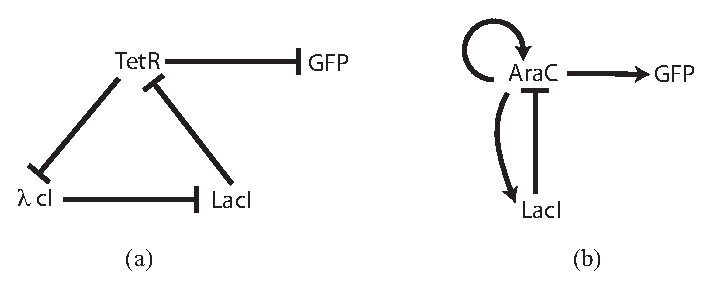
\epsfig{file=figures/oscillators.eps, scale=0.9}
\caption{\label{fig:oscillator}Two different architectures for a
  genetic oscillator. Nodes represent proteins (see
  Chapter~\ref{ch:in-vivo}). Normal arrows mean ``activates the
  production of''. Blunt arrows mean ``represses the production
  of''. (a) A ring oscillator \cite{elowitz-repressilator} called the
  {\em repressilator} consisting of three {\em repressors} connected
  in a ring. (b) A relaxation oscillator consisting of repressors and
  activators \cite{hasty-oscillator}.}
\end{figure}

In synthetic biology, we do not yet know how to build systems that
solve these problems, but we have begun to explore different
architectures for solving specific problems. For example,
Figure~\ref{fig:oscillator} shows two different architecures for
producing oscillations (these are covered in more detail later in this
book). The first is a familar ring oscillator, and the scond is a
relaxation oscillator. Why one would be better than the other in a
given situation will hopefully become clear as we delve into the
details of how they work. 

% The right models and analysis tools
\paragraph{Modeling:} Systems biologists are tempted to write down
equations describing every single reaction in the systems they
study. For example, a recent paper describes a system involving 828
biochemical reactions with 499 ordinary differential equations (ODEs)
with 229 (unknown) parameters \cite{large-model}. This model is fitted
to typically scant data obtained in the lab to obtain estimates of
what the parameters are. The authors also note that the behavior of
the system is insensitive to changes in a number of parameters (taken
one at a time) and infer that as a result they ``know'' some paramters
better than others.

Several fundamental problems with using enormous models are
immediately clear. First, we don't really know good models of even
single reactions inside cells -- their structure is always an
approximate (e.g. is it bimolecular, cooperative, etc.?) and the
reaction rate constants are pretty much impossible to measure. In
fact, the structure of these reactions typically come from what
studies in which a gene is turned off aritifically and the behavior of
other genes is observed to determine causality. When there is
causailty, a reaction is included in the model, whether the
interaction is direct or indirect, fast or slow, etc. Thus, a
collction of even three such ``reactions'', let alone hundreds, is
suspicious. Second, once a system of ODEs is large enough, it is
usually possible to fit almost any finite data set. Therefore, fitting
does not validate or invalidate the model. One may as well fit a
neural network to the data! Finally, modeling and then fitting is
merely {\em descriptive}, not {\em predictive}. A model is really only
useful if it can help you do something (like $F=ma$ helps design
spacecraft trajectories) or makes a scientific prediction that
suggests further experiments.

Many systems biologists are now taking a more pragmatic view of
modeling. One idea, roughly, is to pose the simplist model that both
explains that data at hand and that is useful for predicting data in
new situations\cite{avano}. This is an engineering approach called
{\em system identification} and has been used successfully for decades
outside of biology. Within biology, the approach is viewed with
suspicion: what good is a simple model if it does not account for
every moving part in the system? Another idea is to ask {\em
  qualitative} questions about
networks\cite{zero-deficiency,monotonic-networks}. For example, one
can show that networks without feedback loops are incapable of
oscillating or that there exist a broad set of parameters that do make
another architecture oscillate. This information could be used by the
synthetic biologist to design an oscillator for which there is some
hope of tuning it into place. Yet another approach is to actually
automate the scientific method by designing experiments that are
guaranteed to eliminate as many candidate models as possible
\cite{georgiev-klavins-descrimination}. Such an approach could be
coupled with the design process much as a debugger is coupled with a
compiler.

% Building robust behaviors
\paragraph{Robustness:} Living systems are incredibly robust to
variable nutirent supplies, temperature changes, toxins, mutations,
new competitors, and on and on. Human technologies can be robust too,
or not. Your typical compact car can take all sorts of abuse, but a
the free laser pointer I just got as a freebie at a conference will
probably last about a week before if falls apart. What exactly makes a
system robust is an incredibly subtle question and is asked in all
fields of biology and engineering (in fact, it is one of the primary
questions that brings the two fields together). Control systems
engineering is one of the only fields, however, to actually have
devised a formal, mathematical notion of robustness. Roughly, a system
is {\em robust} to a given {\em perturbation} if its behavior degrades
gracefully as the intensity of the perturbation increases
\cite{robust-control}. Robust behavior in the face of large discrete
changes, however, is still a subject in need of attention.

For synthetic biologists, the most immediate challenge may not be
designing robust molecular systems. Instead, the real challenge is to
understand why and how biological systems are robust. Much of systems
biology concerns this question
\cite{heat-shock,calcium,more-robustness-papers} and successful
explanations there promise to greatly inform the designs of synthetic
biologists.

% Using stochasticity
\paragraph{Stochasticity:} Imagine a computer each of whose bits in
RAM randomly flip from 0 to 1 and from 1 to 0 several times a day
(meaning that the number of flips per second is huge). Such a computer
would have to be programmed very differently than computers
today. Unfortunately, randomness is all over the place in cells. It
arises from several sources. First, because cells are small and
molecules are even smaller, thermal fluctuations are actually quite
large compared with signal intensities. A chemical reaction, for
example, is just a description of the random event that the reactants
happen to combine in just the right geometry to react, the randomness
arising from the giggling and jostling of the reactants and all the
other molecules in the cell. This kind of ``noise'' is called {\em
  extrinsic noise}. Second, the number of molecules of any given type
(called the {\em copy number} of the molecule) inside a cell may be
quite small, say from zero to 50 at any given time. The event that one
of those molecules reacts with another is also a random process. This
kind of randomness is called {\em intrinsic noise}. 

Stochasticity can be readily seen in single cell observations
\cite{elowitz-single-cell}. Isogenic cells with essentially the same
initial conditions can diverge in their behaviors within a relatively
short period of time, due only to the random interactions of the
molecules inside of them. Stochasticity is both compensated for and
exploited by single cells. For example, the process of {\em mitosis}
(cell-replication) has to have very little randomness in it to produce
an essentially identical copy of a dividing cell, and much of the
circuitry responsible for this behavior is presumed to minimize errors
\cite{error-correction-in-mitosis}. On the other hand, randomness may
be used by populations of cells to diversify strategies. For example,
soil bacteria deside to either become {\em competent} (take up DNA
from the environment) or not using essentially a genetically encoded
coin-flipping mechanism \cite{elowitz-b-sub}. The result is that a
precise percentage of a population of such bacteria will be competent,
while others continue to grow. In a fluxuating environment, such a
strategy might be the best bet to ensure survival. (THIS SHOULD BE A
DIFFERENT EXAMPLE). 

Synthetic biologists need to learn to compensate for and use
stochasticity as well. For example, a fundamental question is how does
noise propogate through biochemical reaction networks. If an
intermediate signal is noisy, how is that noise suppressed in the
ouput \cite{avano-noise-cascade}? Also, engineers have found great
uses for random number generators in computer codes (e.g. in
security). How can we make and employ random number generators in
cells?

% Debugging
\paragraph{Debugging:} Electrical engineers use oscilloscpes and
network analyzers to characterize and debug circuits. Computer
scientists use debuggers and runtime analyzers to find bugs. What do
synthetic biologists use? It turns out to be very difficult to
determine what is actually happening is a cell. The information that
is ideally required is a core-dump: we want to know the copy number of
every kind of molecule in the cell as well as its state
(e.g. phosphorylated or not, how it is folded, what it is attached to,
etc). Unfortunately, we can't get this information. But there are
several things we can do. We put GFP and similar reporters (there are
about six colors available) that we can see. We can tag proteins with
molecules that fluoresce in some situations but not in others
\cite{msb-fre-study}. We can take a population of cells and sort it by
size, color, and fluorescence intesnsity \cite{facs}. We can kill the
cell or, more commonly, a population of cells and measure the amount
of RNA or protein to determine which genes were on just before the
cell was killed. We can watch cells grow under the microscope and even
see where certain proteins are being expressed. Every year more
techniques for seeing what is happening inside cells are invented. But
it is likely that we will be in the dark about most of what is going
on inside cells for a good long time. 

Synthetic biologist can respond to this rather fundamental limitation
in a different ways. One idea is to focus on engineering debugger
circuits that could be included in easy to use strains of
bacteria. The idea would be that the cells have built into them
standard debugging tools that can be turned on or off by external
signalling. This is pretty far out, but gives a flavor of what is
really required to do solid engineering with cells. A more down to
earth idea is to carefully ask the question: Given that there are a
limited number of reporter molecules (such as GFP) that can be used at
any given time, where should they be put with respect to a new
proposed design to yield the maximumn amount of information? And more
generally, what information about the behavior of the cell can be
infered from a dynamic trace of those reporter molecules? Recent work,
for example, demonstrates what information can be gleaned from just
the noise characteristics of gene expression
\cite{murray-noise,thorsely-egbert-klavins-in-progress}.

% Preventing systems from being evolved out (Sean's data about # of generations)
\paragraph{Evolution Again:} Recall the discussion above concerning
evolution: It is a fundamental problem in synthetic biology that the
systems we build will be deployed in evolving populations. We desire
two things. One, the systems we build do not get evolved away; and
two, the systems we build do not evolve into something we cannot
control. For the time being, the main problem in synthetic biology is
the former \cite{evolve-away}. Primarily, dropping circuits is a
fantastic strategy for a population since the circuits we so far know
how to design put such an enormous metabolic load on the cell. As we
get better at synthetic biology, expect more graceful circuits that do
not interfere with normal processes. Even then, however, evolving-out
will be a problem. A further improvement is to couple the behavior of
the desired circuit with the very survival of the cell. For example,
suppose that the cell is grown in antibiotics (a ver common way to
test for successful incorporation of a synthetic gene is to also add a
gene encoding for an antibiotic). Next suppose that part of the normal
functioning of parts of the synthetic circuit is to build parts of an
antibiotic protein and assemble it. If any part of the circuit drops
out, the antibiotic is not made and the cell cannot survive. This idea
is similar to the idea of protecting software from being copied or
changed by having it occasionally compute a checksum of its own bits
and aborting if the checksum does not add up.

\section{The Ethics and Risks of Synthetic Biology}

% example: risks of plastic eating bacteria
Synthetic biology has the potential to change everything, for the
better or otherwise. New life forms or new variants on existing life
forms could be dangerous, either accidentally or intentionally. Many
people question whether synthetic biology should be studied at all,
given its {\em dual use} nature. The question is, should we be allowed
to engineer living systems? One answer is, I think, is that {\em we
  already do engineer living systems} -- just not very carefully. 

In fact, we use living systems in a number of ways to positively
impact our health and economy. Bacteria help process nutrients in our
guts and digest waste in landfills. Spiders control insect
populations. Bees pollinate our crops. Algae help supply the world
with oxygen. Exotic trees in the Amazon might produce molecules that
help us treat diseases. It almost seems as if these organisms are in
our service. On the other hand, you can get a tapeworm, bacterial
meningitis, herpes, HIV, the flu, and a whole host of other nasty
problems if you interact with the natural world in an unlucky
way. Furthermore, locusts could eat your crops, termites can eat your
home, or a goose could fly into the jet engine of your airplane to
Boise.

In any case, some of the things we have done technologically and
socially over the last several thousand years have resulted in vast
changes to the natural world that, to date, are far more significant
than changes due to direct genetic tweaking. And the rate at which we
are altering the environment by non-genetic means is increasing. When
the environment is changed and a new niche emerges, some part of the
natural world adapts or possibly collapses – sometimes very
quickly. Examples: The use of pesticides has resulted in new strains
of more virulent pests. The use of antibiotics has resulted in more
virulent strains of infectious bacteria. Our traveling the world in
airplanes has allowed for completely new ways for infectious diseases
to spread. Our use of artificial sweeteners may have made many people
obese. It is very likely that many emerging infectious diseases and
conditions will result directly from new niches that were accidentally
created by for some totally innocuous sounding purpose.

The point is that our current understanding of everything from ecology
to molecular biology is not sufficient for us to begin to evaluate the
introduction of a new policy or technology (even if it does not seem
to be directly related to genetic engineering) in terms of its impact
on the well-being of our species. That is a frightening world to live
in because we are not in control.

Furthermore, nature is designed to manipulate genetic information very
well already. When a population of bacteria finds itself in a new
niche (such as in a moist air-conditioning duct in an office building
or the bilge water of a cargo ship) having strange new nutrients or
surprising new stresses, the population evolves -- often very
quickly. The population of bacteria does this in what seems like a
directed way, but it is really ``just'' evolution. Now, evolution is
simple to describe, but it can move in surprising directions in
seemingly deliberate ways as we discussed above. While still “obeying”
the laws of evolution, bacteria have evolved techniques to evolve
quickly and without merely randomizing their genomes. For example, a
recent paper in Science showed that when a population of {\em
  Streptococcus pneumoniae} is subjected to antibiotics, the bacteria
in the population begin to share DNA among each other
\cite{strep-evolve}!  This allows each bacterium in the population to
try out new genes to fight antibiotics like you might try out a new
piece of shareware from the Internet to combat adware.

We are surrounded by many other examples of rapidly evolving organisms
that seem to have a greater facility with genetic engineering than we
do (they are better at directed exploration to be more exact). HIV and
avian flu evolve very quickly within each host they infect, thereby
adapting to the host and possibly to a treatment regimen. What’s more,
microorganisms evolve much more quickly than we do as a species
because their life spans are shorter. In contrast to humans, who seem
to be at the mercy of their biological environment, the natural world
is actually very adept at surviving and even flourishing in the face
of dramatic changes and attacks.

But our technology evolves for us. Computers evolved from massive,
single purpose beasts the size of buildings to sleek personal digital
assistants that inhabit our pockets (the PDA is just one family of
computer among many flourishing today). Automobiles, agriculture,
buildings, financial markets, power plants, warfare, chewing gum, and
arthritis drugs have all undergone similar evolutions from crude
beginnings. All of these technologies augment (or at lease change) our
ability to survive in the natural world. Not much about us genetically
speaking enables us to live in almost every part of the globe (except
our brains). It is our technology and accumulated knowledge that
enables us to survive mat present levels. Our technology is now
allowing us to re-program living systems directly -- which is a
fundamental shift in the place of humanity in the universe. 

If technology is truly subject to
mutation and selection, then its development is essentially a random
process. New technologies are developed, by engineers, based on old
ones that work well. Customers use products that serve their current
needs. Old technologies become obsolete and eventually extinct. Even
better, our technology is co-evolving with us and with other life
forms on our planet. However, just as biology is more likely to move
in some directions than others, we ourselves can, to some extent,
control the direction that our technologies evolve (with policy and
planning). By better understanding the natural world and our place in
it, we can develop technologies that make us safer, healthier, and
happier. Synthetic biology is hopefully one of those technologies.

Of course, any sufficiently new and powerful technology has risks that
need to be understood and managed. One of the startling aspects of
synthetic biology (which is also what makes it fun to study) is that
new potential applications (safe or otherwise) seem to pop up every
day. Therefore, we simply do not know what we (or someone else) will
be able to build tomorrow. Furthermore, the technology required to
build something new in this field is suprisingly simple, making it
available to anyone. How the uses of synthetic biology should be
regulated is a difficult and open question. Two most-likely unworkable
ideas present themselves. First, synthetic organisms could be
regulated like toxic chemicals. Second, synthetic organisms could be
regulated using the existing bio-safefty regulations for infectious
agents (from {\em Salmonella} to the 1918 flu). Only laboratories
capable of confining such organisms would be allowed to work on
them. Both of these options are problematic because they view the
organisms as the risk. In fact, it is the information -- merely a
sequence of $A$, $T$, $C$ and $G$s -- that really defines a life
form. Technologically, we are close to the day when almost anyone will
be able to boot up a new organism starting only with the genetic code
defining it.

Thus, what really needs to be considered, is how to keep track of the
information, the code, and thre recipes of synthetic biology. A good
analogy is with computer viruses. If you look up computer viruses on
the Internet, you will find all sorts of descriptions on how to make
them. Furthermore, you can find manuals on how to program in a variety
of languages, and specifications of network protocols and operating
system APIs to help you write very cool Internet applications, and
also very nasty computer viruses, worms, trojan horses, and the
like. The equivalent information for living systems is now being
generated, compiled, and disseminated. But it is one thing to bring
the Internet down, and another to bring the biosphere down.

Thus, among the goals of synthetic biology should probably be to (a)
to understand in what ways synthetic biology is the same and different
from existing bio-technologies so that it can be regulated; and (b) to
understand how to recognize or test for the potential impact of a new
technology on exiting life. The latter requires really a new,
quantitative (and I would argue, engineering-based) understanding of
living systems.

\section{Overview}

This text is an attempt to provide a foundation for the design,
modeling, and analysis of synthetic biological systems. It focuses
primarliy on aspects of dynamical systems and control. The goals are
essentially: (1) introduce the theoretical issues of synthetic biology
to students studying control engineering; (2) introduce control and
dynamical systems to students studying synthetic biology; (3) to
prepare students to understand the research in the area so that they
can begin to contribute to the field. The text does not cover many
other very important issues in synthetic biology, such as experimental
techniques, or logic and computer science. We are preparing a
laboratory manual the {\em does} introduce basic genetic engineering
with bacteria, that is available online.

We assume a minimal background in dynamical systems (basic
differential equations, linear algebra, and probability) and
essentially no background in biology -- although an undergraduate
course in biochemistry would be very helpful. 

The topics included in the text are geared toward understanding the
behavior of systems that researchers have actually built or systems
found in nature that have been well characterized. The goal is to
focus on systems that have some hope of being implemented and the
theoretical issues associated with getting them to work -- as opposed
to more speculative ideas and architetures that are (presently) only
of abstract interest.

Therefore, the topics include the following. First, we give a very
high level overview of the operation of procaryotic cells to ground
the discussion of specific systems later. We give an overview of
synthetic biology {\em in vitro}, as an alternative experimental
reality. There is a breif review of differential equations, mostly to
remind the reader and set notation. Then we discuss the main models
used in systems and synthetic biology, namely mass action kinetics,
enzyme kinetics and stochastic kinetics. The approach to enzyme
kinetics is somewhat different than in other texts in that we first
introduce the {\em singular value perturbation} method from nonlinear
systems, and then show how to apply the method to mass action kinetics
models to obtain enzyme kinetics models. We also discuss the potential
for the misuse of enzyme kinetics models.

As discussed above, models in synthetic biology are to be viewed with
suspcion, primarily because there are no well-established first
principles from which to derive models. Typically the theory of
chemical kinetics is applied to the reactions inside a cell, but the
assumptions required by chemical kinetics are not really met
(well-mixedness, point mass molecules, 3D difussion, etc.). Therefore,
we describe how to evaluate how good a model is and how to obtain
models from data. In particular, we discuss the composition of systems
and what can go wrong; robustness and sensitivity; and parameter
estimation and system identification.

\section{Problems}

\begin{exercise}
  Recall the five capabilities we associate with living systems:
  sensing, actuation, control, information storage, and
  evolution. Which of these capabilities does a car have? How is the
  capability instantiated? What other technologies have these
  capabilities?
\end{exercise}

\begin{exercise}
  Visit the {\em Kyoto Encyclopedia of Genes and Genomes} at
\begin{quote}
  \ \\
  \href{http://www.genome.ad.jp/kegg/}{\tt http://www.genome.ad.jp/kegg/}
  \ \\
\end{quote}
  and search for ``butanol''. Find where
  it says ``Compound'' and click on the first compound. Then click on
  the pathway for Butanoate metabolism. If you have a microorganism
  that synthesizes Butanoyl-CoA, enzyme could you use to
  get Butanoate? What organisms could you get the gene for this
  enzynes from (an exhaustive list is not required)?
\end{exercise}

\begin{exercise}
  Describe a technology with which you are familar. In what ways is it
  robust? In what ways is it fragile? How have designs of the
  technology evolved to become more robust? 
\end{exercise}

\begin{exercise}
  Look up the {\em International Genetically Engineered Machine}
  (iGEM) competition using your favorite search engine. iGEM is a
  synthetic biology competition for undergraduate teams. Look over the
  team wikis from years past and find (a) a medical application; (b) a
  biofuel application; (c) a components-based (e.g. genetic logic
  gates, amplifiers, etc) project. Describe each project briefly and
  speculate what engineering principles might be brought to bear on
  the problem.
\end{exercise}

\begin{exercise}
  Look up the {\em Obligation of the Engineer} using your favorite
  search engine. It describes what responsibilities engineers have
  when practicing their art. How could this oath be changed into an
  {\em Obligation of the Synthetic Biologist}?
\end{exercise}

\chapter{Basic Biochemistry} \label{ch:bio}

\section{{\em E. coli}: The Model Procaryote}

% What it is
Synthetic biologists work with a variety of organisms. The choice of
which organism depends on the application in mind and also on the
innate abilities of the organism. For example, if the goal is to
produce butanol from sunlight, an organism that photosynthesizes and
that normally produces some useful immediate precursor to butanol is
an appropriate starting point (for example, the {\em
  cyanobacteria}). If the goal is to develop a medical treatment, a
simple eukaryote (such as the yeast {\em S. cerevisiae}) would be
appropriate. For our purposes, which are to design and debug basic,
portable biochemical circuits and regulatory processes, the ideal
organism is the humble bacterium {\em Escherichia coli}, or {\em
  E. coli} -- shown in Figure~\ref{fig:ecoli}. 

\begin{figure}
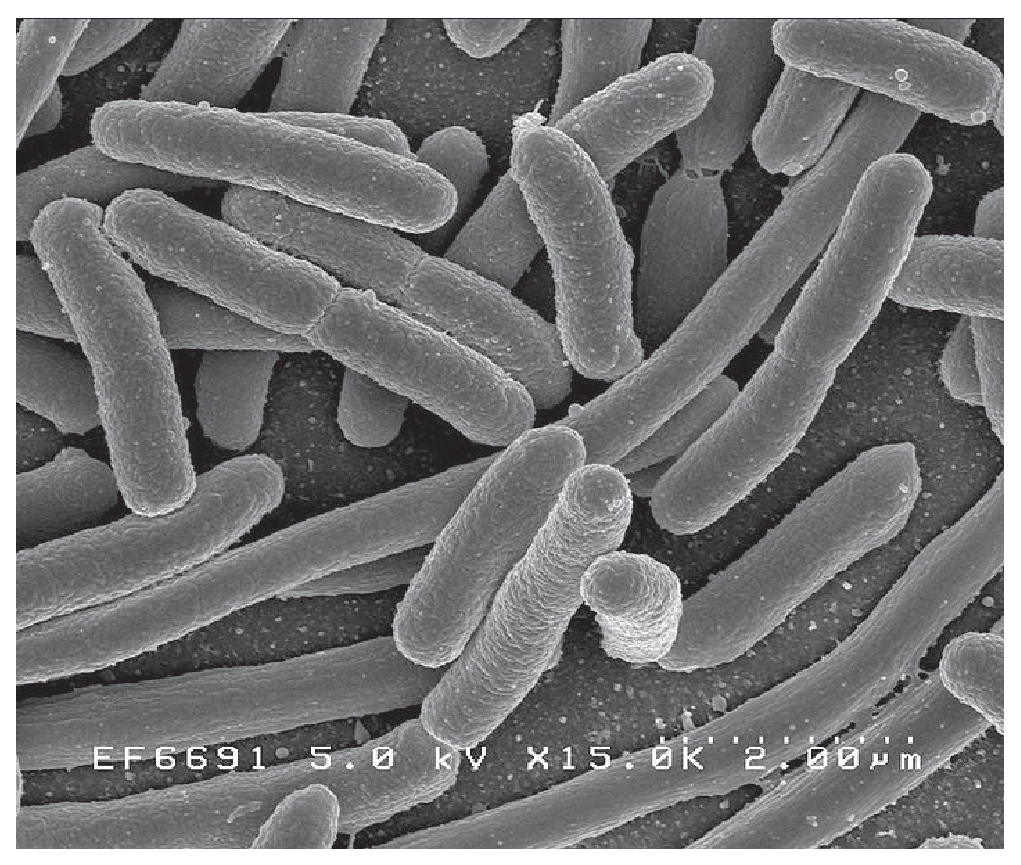
\epsfig{file=figures/ecoli.eps, scale=0.6}
\caption{\label{fig:ecoli} A scanning electron micrograph image of
  {\em E. coli} cells. Each cell is approximately 2 $\mu$m long and
  has a volume of about 1 $\mu\mathrm{m}^3$. Several of the cells in
  this image have just divided end-to-end, producing genetically
  identical daughter cells. Credit: Rocky Mountain Laboratories,
  NIAID, NIH. }
\end{figure}

{\em E. coli} is very well studied. Many of the most important genetic
and molecular processes in biology were first discovered in {\em
  E. coli}, and at least eight Nobel prizes are associated with
discoveries made with it (e.g. Monod, Lederberg, Taum and Beadle,
...). {\em E. coli} is, furthermore, the workhorse in almost every lab
that uses DNA: It is used basically as a DNA factory -- happily
replicating any DNA you put into it. {\em E. coli} are used in
industry as well. For example, the production of insulin, which used
to be obtained from pig pancreases, is now done in genetically
modified {\em E. coli} \cite{insulin}. Because {\em E. coli} is so
well understood, if {\em you} want to know how something in {\em
  E. coli works} so that you can hack it, you will more often than not
be able to find someone to help you. In contrast, if you work on an
obscure microorganism, and you will most likely be on your own.

{\em E. coli} is found naturally in the human gut, along with numerous
other kinds of bacteria. Humans can't live without their bacteria,
which help them digest their food, among other responsibilities. Most
of the cells on and in your person, in fact, are (very small) bacteria
cells and not (big) human cells. The strains of {\em E. coli} used in
the lab are all descendants of {\em E coli} K-12, which was isolated
at Stanford University 1922 from human feces. It was kept there for
years as a stock strain and has, in fact, evolved to live alone in the
comfort of the lab. Due to their relaxed lifestyle, K-12 can barely
survive outside of the lab and is generally considered to be harmless
(unlike the strains of {\em E. coli} that sometimes infect foodstocks
\cite{taco-bell}). You can now obtain from a variety of sources a huge
range of strains related to K-12, each with its own ``features''. Some
strains produce lactose digesting enzymes, some can conjugate with each
other, some have had their DNA repair genes knocked out, and so on
\cite{cgsc}.

To some extent, if a synthetic biologist can get a device to work in
{\em E. coli}, the principles of how its works should apply to other
organisms as well and often the circuit can be transplanted as is into
other organisms. As Jaques Monod said, ``All that is true for the {\em
  Colon bacillus} [e.g. {\em E. coli}] is true for the elephant''
\cite{monod}. Monod's observation is that all life forms on earth use
essentially the same architecture -- of which this chapter is an
overview.

In particular, this chapter describes, at a very high level, the
architecture of organisms like {\em E. coli} -- that is {\em
  procaryotes} (cells not having a nucleus). The goal is to ground the
ideas that appear later in the book in systems inside a
well-understood model organism. Note that this chapter is not even
remotely a good substitute for a textbook on biochemistry
\cite{nelson-cox}, a textbook on cell biology \cite{thecell}, or a
text book on bacterial genetics \cite{bact-genetics}.

\section{Molecules in the Cell}

Bacteria, including {\em E. coli}, are single celled {\em procaryotic}
organisms. Among other things, this means that they do not have a
nucleus containing their genomic DNA, and they do not have
particularly sophisticated ways of processing their RNAs and
proteins. Rather, the DNA and most of the other molecules that make up
an {\em E. coli} cell's machinery, are located in the main interior of
the cell called the {\em cytoplasm} or they are part of the cell {\em
  membrane} enclosing the cytoplasm. In this section we describe at a
high level what most of the important molecules are called and what
they do in the cell. It is difficult to know where to start with such
a description as each type of molecular interacts with other types so
that in describing RNA, we need to talk about DNA and proteins, for
example. The order of presentation below is therefore somewhat
arbitrary. The reader might consider reading this section twice to
resolve references to one type of molecule while introducing another
type of molecule.

% Molecules (DNA, RNA, Protein, small molecules, etc) 

\paragraph{DNA} Perhaps the most important kind of molecule in the
cell is {\em deoxyribonucleic acid} or DNA. A big DNA molecule, called
the genomic DNA, stores almost all of the information required to
build and run an {\em E. coli}. DNA molecules are long, oriented
polymers (long chains) of four different types of {\em nucleotides},
as seen in Figure~\ref{fig:dna}. Each nucleotide consists of a {\em
  base}, adenine (or A), thymine (or T), guanine (or G) and cytosine
(or T), attached to a deoxyribose sugar, and a phosphate group. The
nucleotides in a DNA molecule are strung end to end to form a long
chain or, more often, a circle. Since the nucleotides in a DNA molecule
can appear repeatedly and in any order, there are in fact $4^N$
different DNA molecules of length $N$. For a standard strain of {\em
  E. coli}, $N \approx 4.6$ million. If we were to randomly
make DNA molecules of this length and try to ``boot them up'' inside a
cell, the chance we'd accidentally make a working organism like {\em
  E. coli} is approximately one in $4^{10^6}$. Apparently, we need to
understand how to put together (or program) DNA molecules more
systematically.

\begin{figure}
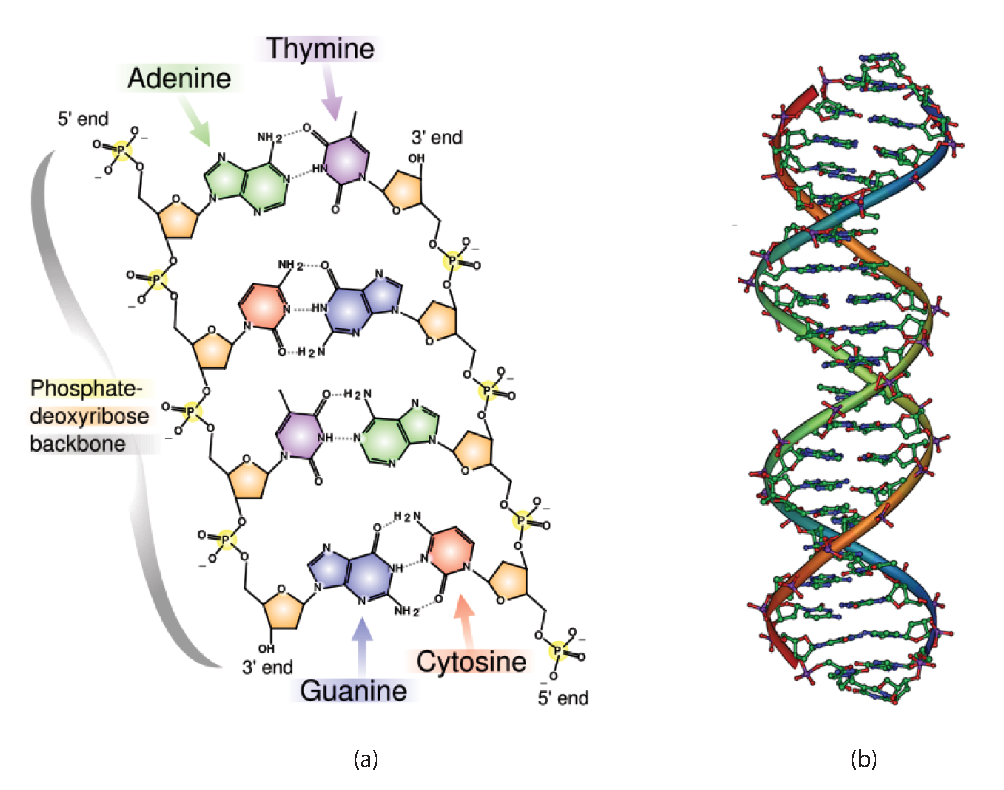
\epsfig{file=figures/dna.eps, scale=0.75}
\caption{\label{fig:dna}The structure of DNA. (a) Bases and base
  pairing. DNA consists of polymers of bases of four different types:
  adenine (or A), thymine (or T), guanine (or G) and cytosine (or T)
  each attached to a deoxyribose sugar. Two stands of DNA will form a
  duplex if they are complimentary: A sticks to T and C sticks to
  G. Note also that DNA has an orientation: the 5' end is different
  than the 3' end. (b) The double-helix. Double stranded DNA folds
  into a double-helix the 3D structure of which can form highly
  specific binding sites for regulator proteins.}
\end{figure}

DNA molecules are typically not found alone. Instead each DNA strand
is attached, with {\em hydrogen bonds}, to a {\em
  complimentary strand} via {\em Watson-Crick} base pairing. It turns
out that A sticks to T and C sticks to G, so the strand $5'-ATAGCA-3'$
is complimentary to $3'-TATCGT-5'$. In this notation, the strands are
oriented from the $5'$ to the $3'$ ends (see Figure~\ref{fig:dna}). It
is this complimentary nature of DNA that makes it ideal for
representing and copying information. If you (or the cell) unzips a
double stranded piece of DNA, each makes a template for the
construction of a new complimentary strand. This copying occurs every
time a cell divides with incredible accuracy: the error rates are
about one mismatch in every $10^9$ bases copied \cite{dna-error-rate}.

In later sections of this chapter, we describe at a high level how 
DNA is interpreted by the machinery in the cell to direct growth,
program how the cell responds to its environment, and so on.

\paragraph{RNA} Although we just said that DNA is the most
important molecule in the cell, it is hard to overstate the importance
of {\em ribonucleic acid} or RNA. RNA is structurally similar to DNA
except that the bases are attached to a ribose sugar instead of a
deoxyribose sugar and instead of thymine RNA contains uracil. The
similarity ends there however. While DNA is a stable information
carrier, RNA is less stable and to some extent defines the changing
internal state of a cell. Furthermore, RNA is generally found single
stranded, often modified by the addition of other small molecules, and
is typically folded up on itself more like a protein, as shown in
Figure~\ref{fig:rna}. Finally, while DNA is a massive circular
double-stranded beast, RNAs are typically short (from 10 to 3000 bases
long).

\begin{figure}
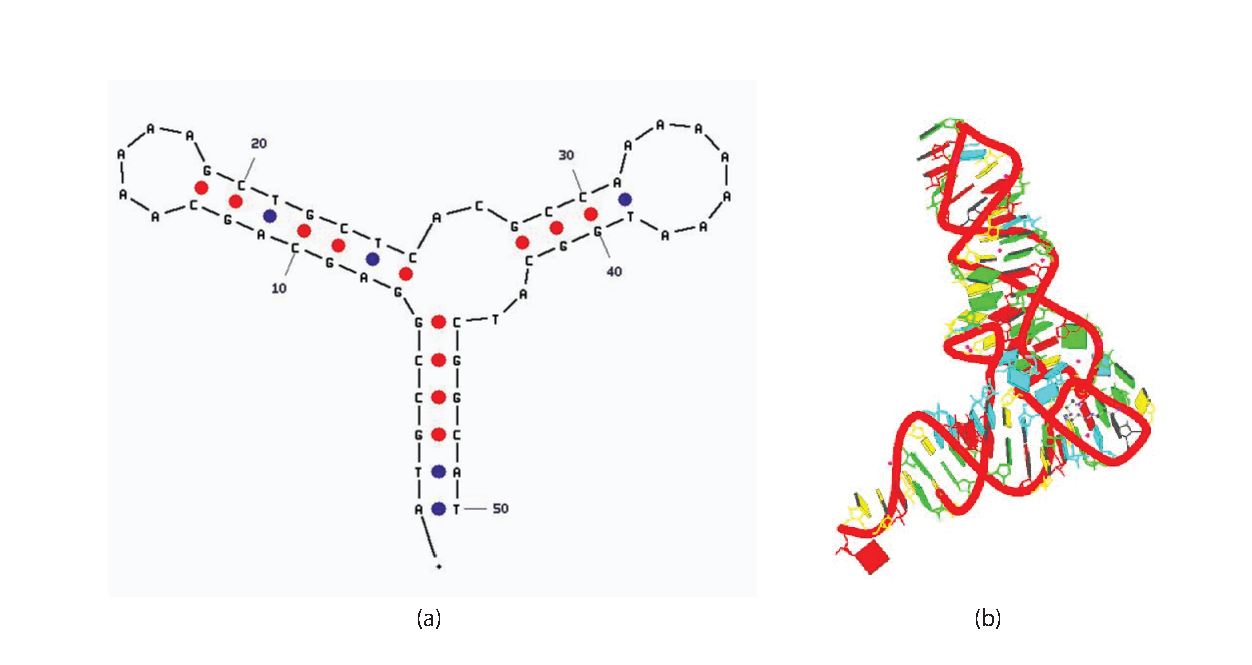
\epsfig{file=figures/rna.eps, scale=0.6}
\caption{\label{fig:rna} RNA. (a) The topology of a typical RNA
  molecule. The RNA strand folds up on itself in predictable ways with
  A sticking to U and C sticking to G. (b) The 3D structure of a
  transfer RNA.}
\end{figure}

All RNAs in the cell are {\em transcribed} (see below) from regions of
the genome called genes. Once transcribed, an RNA is destined for one
of a surprisingly many roles in the cell. {\em Messenger RNA} or mRNA
is an intermediate representation of a protein. Its role is to carry
the information for how to build a protein from the genome to the
protein building machinery. The protein-building machinery itself is
built primarily from two types of RNA called {\em transfer RNA} or
tRNA and {\em ribosomal RNA} or rRNA. tRNAs are the interface between
triples of bases called codons (found on on mRNAs) and the amino acids
corresponding to the codons. Ribosomal RNAs glob together into
molecular machines called ribosomes that translate mRNAs into proteins
using tRNAs (this process is described below). Finally, there
regulatory RNAs of many type. For example, {\em small interfering
  RNAs} or siRNAs are bits of RNA that are complimentary to regions of
mRNAs that prevent their translation into protein. Another type of
regulator RNA are the various {\em ribozymes}, which are RNAs that
exhibit catalytic activity, for example, cleaving other RNAs in
specific (and programmable) regions.

\paragraph{Protein} Proteins are folded up polymers consisting of
chains of sub-units called {\em amino acids}. There are 20 different
amino acids (see Figure~\ref{fig:genetic-code}) that are found in
normal living systems. Amino acids all have the same basic form
consisting of an amino group ($H_3N$) and a carboxyl group ($CO_2H$)
on either side of a $H-C-R$ group. The $R$ is another group called the
{\em residue} that determines the type of amino acid. Each amino acid
is different: it may be hydrophobic or hydophyllic; it may be polar or
not; etc. 

Amino acids can form chains due to their modular nature. The amino
group of one can stick to the carboxyl group of another forming a
peptide bond and releasing a water molecule, as shown in
Figure~\ref{fig:peptide-bond}. By continuing this process, any chain
of up to thousands of amino acids can be formed. Due to the different
chemical natures of the amino acids, the chain will {\em fold up} into
different shapes. The resulting protein will have pockets and grooves
and bumps each with a function determined by the amino acids near that
feature. Thus, proteins are programmed blobs of matter with programmed
chemical functionality -- and the possible functionality seems to be
limitless. Almost every important function inside a cell is performed
in part by a protein. They regulate the expression of genes; help
transport molecules in and out of the cell; a particular protein {\em
  enzyme} can very specifically increase the activity of a particular
chemical reaction; some proteins polymerize into long, rigid chains
that give cells structure; protein motors can pull cargo around inside
cells; some proteins are hormones that carry signals to other cells;
and on and on. This programmability of function is unparalleled.

\begin{figure}
\centering
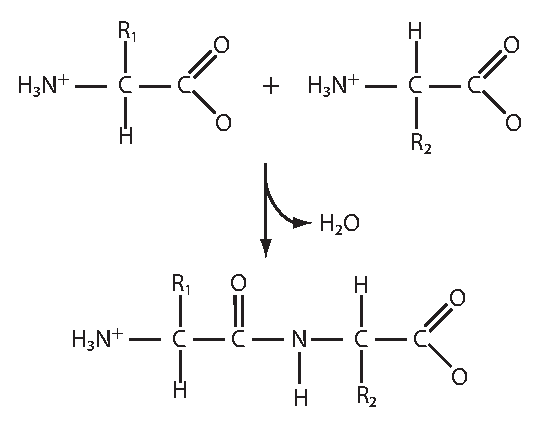
\epsfig{file=figures/peptide-bond.eps, scale=0.8}
\caption{Two amino acids condense to form a peptide bond. Long chains
  of amino acids fold up to form proteins. The amino group of the
  chain is called the N-terminus and the carboxyl group is called the
  C-terminus. \label{fig:peptide-bond}}
\end{figure}

An example protein is GFP, discussed in the introduction. It consists
of a sequence 264 amino acids with a mass\footnotemark of just over 27
kDa. This sequence of amino acids, shown in Figure~\ref{fig:gfp}(a),
folds up into a secondary structure due to the natural attractions and
repulsions of its constituent amino acids, as shown in
Figure~\ref{fig:gfp}(b). Stretches of a protein often form into
recognizable substructures, either $\alpha$-helices or
$\beta$-sheets. The former are helical regions and the latter are
regions that interact with other $\beta$ regions to form sheet like
structures. Figure~\ref{fig:gpf}(c) shows a cartoon of GFP in which helix
and sheet structures are highlighted. Sub-structures that are neither
sheets nor helices are called random coils and are shown as simple
lines are ropes. 

\footnotetext{Masses of molecules are often measured in Daltons
  (Da). One Dalton is approximately the mass of one Hydrogen atom.}

\begin{figure}
\centering
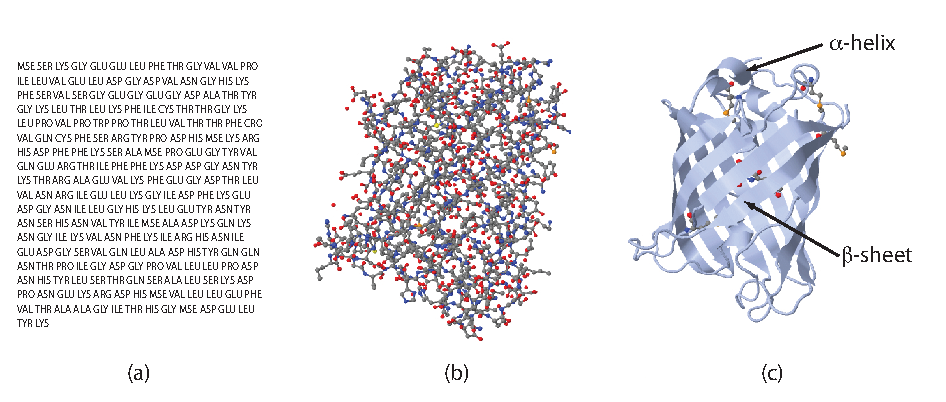
\epsfig{file=figures/protein.eps, scale=0.8}
\caption{The structure of green fluorescent protein (GFP), downloaded
  from the protein data bank. (a) The sequence of residues. Each
  three letter code corresponds to a different residue, according to
  the scheme in Figure~\ref{fig:genetic-code}. (b) The three
  dimensional or secondary structure of GFP. The relative coordinates
  of each residue are typically determined empirically using X-Ray
  crystallography. (c) The cartoon version of the protein showing more
  clearly its structure as a barrel-shaped molecule. \label{fig:gfp} }\end{figure}

\paragraph{Small Molecules} The are an enormous variety of small
molecules in the cell (besides, of course, $H_2O$) that the cell is
very adept at processing. Simple sugars, carbohydrates, lipids,
alcohols, amino acids, nucleotides, signaling molecules and
antibiotics are just some of the substances that cells know how to
make. These molecules are of great interest to metabolic engineers who
see cells as programmable chemical processing plants. By changing the
expression of protein enzymes or by adding the genes for new protein
enzymes into an organism, new substances can be made by old organisms. 


\section{Processes}

\subsection{Transcription}

% Processes: Transcription, translation

The long chain of genomic DNA inside a cell is dived up into segments
called {\em genes}. These genes take on many forms. The most basic
form consists of a short sequence of DNA called a {\em promoter},
after which follows a long sequence (up to thousands of base pairs) of
DNA called a {\em template} containing the information represented by
the gene, and terminated by a short sequence called a {\em
  terminator}. See Figure~\ref{fig:transcription}(a).

\begin{figure}
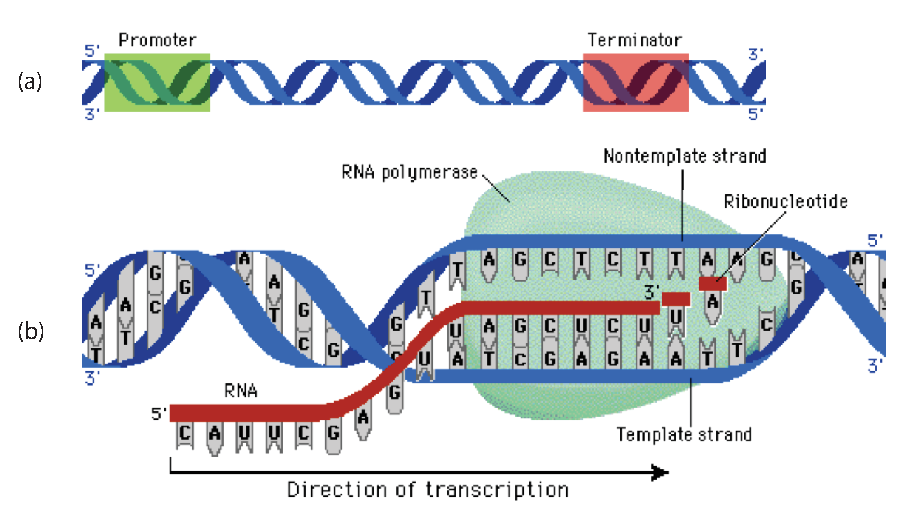
\epsfig{file=figures/transcription.eps,scale=0.75}
  \caption{\label{fig:transcription} (a) A simple gene containing a
    promoter, a template, and a terminator region. (b) The process by
    which RNA polymerase (RNAP) transcribes the template DNA into an
    RNA transcript. }
\end{figure}

The promoter region of a gene has a specific three-dimensional
structure due to the sequence of nucleotides in the region. This
structure allows an important enzyme called {\em RNA Polymerase}
(RNAP) to specifically bind to the promoter region (RNAP is actually a
collection of proteins that act together as an enzyme). Once there,
RNAP locally splits the DNA double helix in the template region and
builds an RNA molecule complimentary to the template. The new piece of
RNA is called the {\em transcript} from the template. In bacteria,
this happens at an astounding rate of about 80 nucleotides per second
\cite{alon-book}. The RNAP continues transcription of the template
until it reaches the terminator, at which point the RNAP falls of the
gene. See Figure~\ref{fig:transcription}(b).

A gene that is ``on'' (see regulation, below) may have many RNAP
enzymes actively transcribing the gene at any given time and so there
may be many transcripts from the gene present in the cell at any given
time. Also, RNA is degraded fairly quickly. The signals and conditions
represented by RNAs are therefore temporary.

The RNA transcripts in the cell have many possible destinies,
summarized below:

\smallskip

\begin{tabular}{lll}
Messenger RNA (mRNA) & \ & mRNA can be {\em translated} into one or \\
                     & \ & several proteins (see Translation, below).  \\
Transfer RNA (tRNA)  & \ & tRNA is the interface between mRNA and protein.  \\
                     & \ & Each type of tRNA is modified to carry a \\
                     & \ & specific amino acid on one end and has an \\
                     & \ & {\em anticodon} on the other end \\ 
Ribosomal RNA (rRNA) & \ & The ribosome is a complex machine consisting \\
                     & \ & of RNA and protein that translates mRNA into \\
                     & \ & protein by stringing together amino acids \\
                     & \ & presented by tRNAs \\
Other                & \ & Other RNAs can fold into RNA enzymes called \\
                     & \ & ribozymes or (esp. in Eucaryotes) form small \\
                     & \ & antisense RNA or micro RNA      
\end{tabular}

\subsection{Translation}

Some of the RNA transcribed has a chance to be {\em translated} into
protein, as long as it doesn't get degraded first or isn't blocked by
some antisense RNA. An mRNA contains a {\em ribosomal binding site} or
RBS to which the enzyme responsible for translation, the {\em ribosome}
binds. Once bound, the ribosome moves forward (in the 5' to 3'
direction) on the mRNA until it encounters the sequence AUG -- the
{\em start codon} and also the codon for Methionine. 

\begin{figure}
\centering

\epsfig{file=figures/genetic-code.eps}
\caption{\label{fig:genetic-code}
(a) The genetic code. The first letter in a codon is at the center. (b) Abbreviations. 
}
\end{figure}

There are other three letter codons as well, after the start
codon. Each codon corresponds to a specific amino acid according to the
{\em genetic code} shown in Figure~\ref{fig:genetic-code}. This code
is almost exactly the same in every organism ever studied -- which is
why a gene from one organism is likely to work when inserted into
another organism. The ribosome steps through each codon starting with
the start codon until it reaches a {\em stop codon}. 

\begin{figure}
\centering
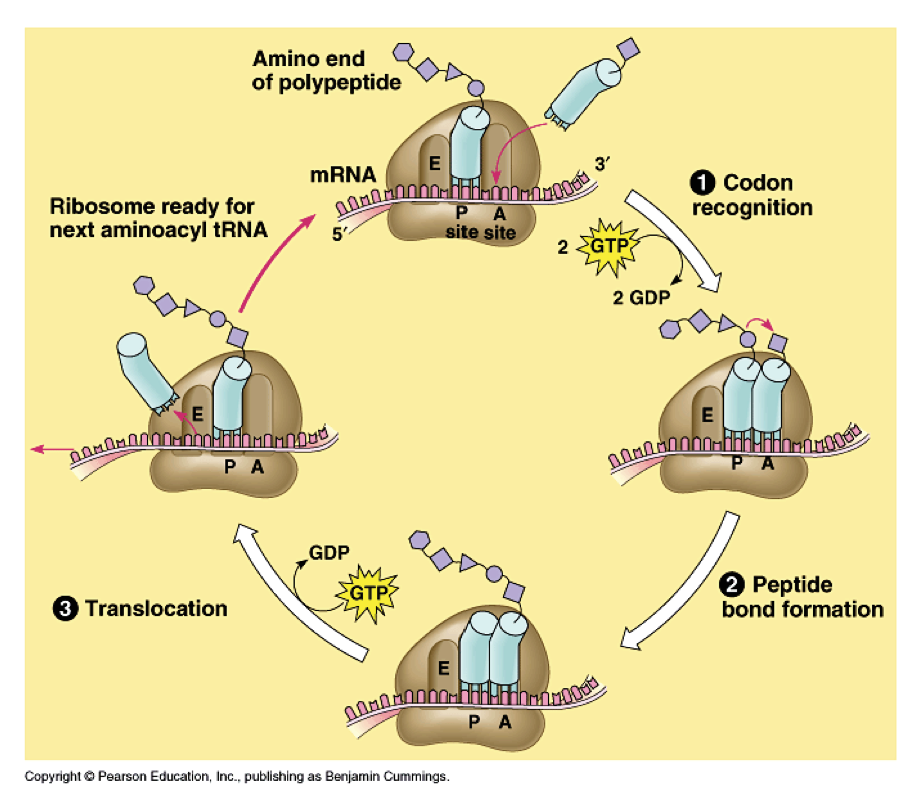
\epsfig{file=figures/translation.eps, scale=0.75}
\caption{\label{fig:translation} The process of translation. The
  Ribozyme binds onto the {\em ribosomal binding site} of an mRNA,
  moves forward to the start codon, and thne translates the codons in the
  mRNA into protein, ending at a stop codon.}
\end{figure}

Specifically, when a ribosome parks at a codon, a tRNA having the
complimentary sequence, the anti-codon, docs at the codon, held in
place by the ribosome. Next, the amino acid at the other end of the
tRNA is attached to a growing chain of amino acids by the
ribosome. Then the ribosome steps forward to the next codon and
discards the transfer RNA (without the amino acid). This process
continues until the stop codon is reached at which point the sequence
of codons in the mRNA has been completely translated into a sequence
of amino acids. The amino acid chain folds up into a functional
protein while it is being translated or very soon after translation ends. 

The ribosome, which consists of several subunits of both rRNA and
protein is arguably the most remarkable molecular machine in the
natural world. Not only are they responsible for translation and
protein biosynthesis, they do their job very well -- correcting for
errors and processing 12 to 21 amino acids {\em per second}. 


In should be noted that transcription and translation, in procaryotes
anyway, occur simultaneously. A given gene may have several RNAP
molecules transcribing mRNAs off of it at any given time. Each of the
mRNAs may have several ribosomes attached to it, translating protein.

\subsection{Regulation}

% constitutive vs regulated
Some genes are on all the time, meaning that RNA transcripts are
constantly generated by RNAP using the template in the gene. Such
genes are called {\em constitutively expressed}. Most genes, however,
are regulated in some way so that the RNA transcripts for the gene are
only generated when they are needed. The most common way for a gene to
be regulated is via proteins called {\em transcription factors}.

\begin{figure}
\centering
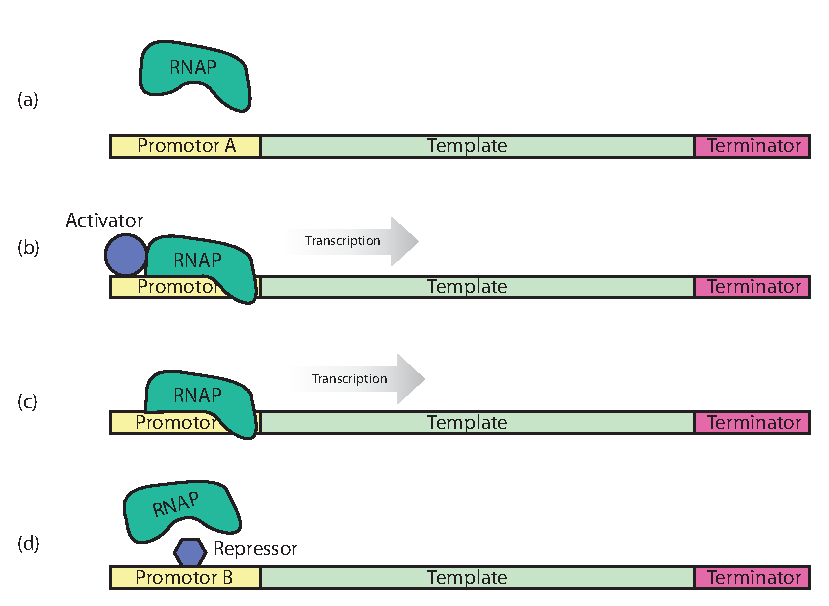
\epsfig{file=figures/regulation.eps, scale=0.75}
\caption{\label{fig:regulation}
  (a) RNAP has low affinity for promoter A. (b) The presence of a
  transcription factor specific to promoter A increases the affinity
  of RNAP for the promoter. (c) RNAP has high affinity for promoter
  B. The presence of a repressor specific to promoter B blocks RNAP
  from transcribing the gene.} 
\end{figure}

As shown in Figure~\ref{fig:regulation}, transcription factors can
either be {\em activators} or {\em repressors}. An activator $A$ works
by improving the affinity of RNAP for specific promoters $p_A$ that
are complimentary to $A$. In contrast, a repressor $R$ works by
blocking RNAP from docking to promoters of type $p_R$. For example,
the $LacI$ repressor (which is actually four identical proteins bound
together into a tetramer) is found in {\em E. coli}. It sticks very
selectively to the promoter $p_\mathit{lac}$ due to the three
dimensional structure of the DNA double helix comprising the
promoter. When bound, it prevents RNAP from binding to the
promoter. In general, promoters and transcription factors go together
and the sequence of $A$, $T$, $C$ and $G$ in the promoter determines a
three dimensional structure in the DNA helix that has some affinity
for RNAP and some affinity for some transcription factors (either zero
or more).

In addition to the above simple mechanisms, many transcription factors
work in groups so that transcription occurs as some function
%
$$
  \mathrm{rate\ of\ transcription}\ = \ f(T_1, ..., T_n) 
$$
%
of the concentrations of the transcription factors $T_1, ..., T_n$
associated with the gene. 

Many transcription factors take on active and inactive forms based on
the presence or absence of small molecules. Such transcription factors
thus form sensors. For example, the repressor $LacI$ is active when
there is none of the sugar lactose around. In its active form, $LacI$
represses the genes encoding the enzymes for incorporating and
metabolizing lactose. In the presence of lactose, the repressor
becomes inactive, and the lactose genes are transcribed (and
translated). In general, there are several ways in which a small
molecule can interact with a transcription factor -- these are
summarized in Figure~\ref{fig:trans-small}.

\begin{figure}
\centering
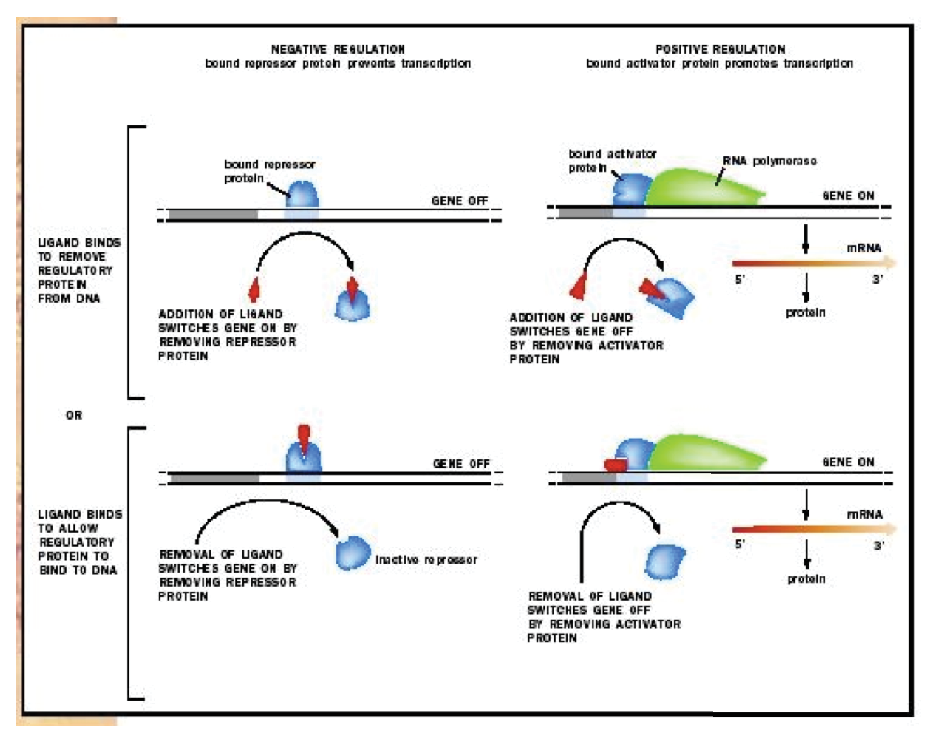
\epsfig{file=figures/trans-small.eps, scale=0.75}
\caption{\label{fig:trans-small}
  Small molecules can activate or deactivate transcription factors in
  a variety of ways. }
\end{figure}

Now consider a set of protein-coding genes $g_1, ..., g_n$. Draw each
gene as a circle. If a gene produces a transcription factor that
activates or represses another gene, we write an arrow or a line with
a bar respectively from one gene to the other. If a small molecule
activates or deactivates a transcription factor, we draw similar
arrows from nodes representing the molecule to the arrow representing
an interaction. The result is a {\em genetic regulator network}, and
example of which is shown in Figure~\ref{fig:grn}. 

\begin{figure}
\centering
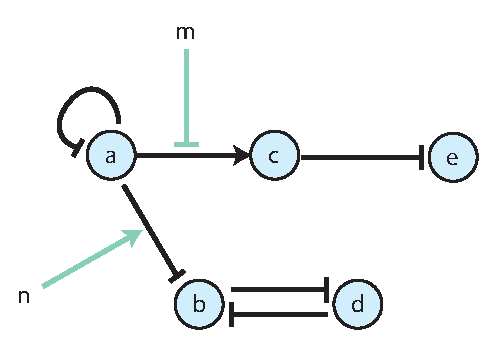
\epsfig{file=figures/grn.eps}
\caption{\label{fig:grn}
  Small molecules can activate or deactivate transcription factors in
  a variety of ways. }
\end{figure}

There are a host of other ways in which genes are regulated, not
always by proteins. For example, non-coding RNAs can interact with
mRNAs in a variety of ways, either preventing the mRNAs from being
transcribed, or even by allowing them to be transcribed. A good survey
of these mechanisms can be found in \cite{rna-synthetic-biology}.

\subsection{Metabolism}

A cell is a miniature chemical processing plant. Most cells can
synthesize a broad variety of substances from the raw materials they
take up from the environment. For example, {\em E. coli} can
synthesize, among other things, amino acids for protein construction,
nucleotides for RNA and DNA, and carbohydrates for energy
storage. Furthermore, the substances that cells take up are highly
variable, so many of the chemical reactions inside cells are designed
to break down nutrients into key energy carrying molecules (such as
ATP) and basic raw materials for later synthesis reactions (such as
pyruvate). Figure~\ref{fig:metabolism-overview} illustrates the
process of {\em catabolism} (breaking down nutrients) and {\em
  anabolism} (synthesizing) useful molecules. 

As described above, many proteins act as enzymes. An enzyme is a
catalyst that increases the backward and forward rate of a chemical
reaction (or family of reactions) by lowering the energy barrier
between the reactants and the products. By expressing some protein
enzymes and not others, the cell can steer metabolites through desired
pathways. Furthermore, by sensing metabolites (for example with
transcription factors that are activated by metabolites), a genetic
regulatory network can {\em control} the metabolism. 

\begin{figure}
\centering
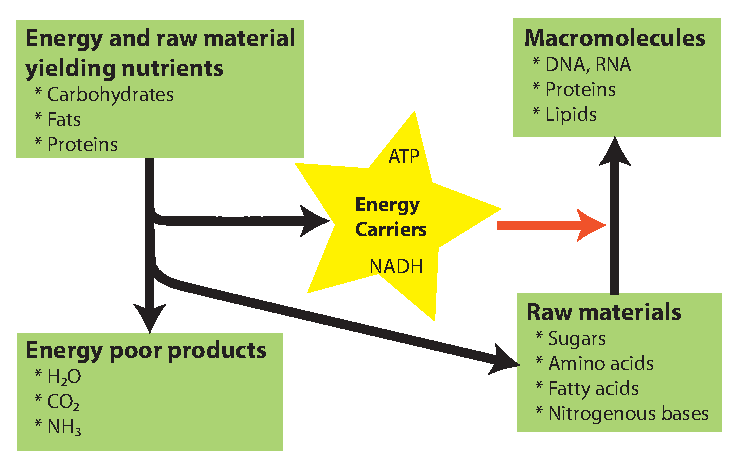
\epsfig{file=figures/metabolism-overview.eps, scale=0.7}
\caption{\label{fig:metabolism-overview}
  Metabolism ... }
\end{figure}

A complete description of all of the metabolic pathways in even {\em
  E. coli} is beyond the scope of this (and most other) texts. There are
an enormous number of metabolites and reactions. However, to give a
flavor of what is involved, we briefly describe a key metabolic
pathway that is fundamental to life, namely {\em
  glycolysis}. Glycolysis is found in every organism on the planet and
likely evolved very early.

The glycolytic pathway (glycolysis) essentially is responsible for
converting the sugar {\em glucose} into two molecules of {\em
  pyruvate} with a net gain in energy of two ATP molecules. Glucose is
a basic nutrient that can either be taken up by the cell from the
environment or obtained from carbohydrate energy storage. It has three
main destinies in the cell: (1) It can be put into storage; (2) it can
be used in the synthesis of small molecules such as nucleotides and
amino acids; (3) it's high-energy content can be used to make
ATP. The first step of the third destiny is glycolysis. Pyruvate, the
product of glycolysis, is still energetic and itself is a precursor
for several pathways, the most important of which is the citric acid
cycle, which milks the rest of the energy out of pyruvate by oxidizing
it.

The glycolysis pathway is shown in Figure~\ref{fig:glycolysis}. It
consists of a series of several steps. The names of the metabolites
are shown. Each one consists of a minor change to the metabolite
before it. In some steps ATP (adenosine triphosphate) is consumed to
produce ADP (adenosine diphosphate), which is an energy consuming
step. In other steps, ADP is consumed and ATP is produced. In the fifth
step, energy is also produced via the {\em cofactor} NAD$^+$. This
molecule is a cofactor of many steps in the metabolism of the cell
and, after ATP, is one of the most common players in metabolic
pathways. 

Each step in the pathway is labeled by the name of the enzyme
associated with the reaction. For example, the last step is catalyzed
by the enzyme {\em pyruvate kinase}, which increases the rate of the
reaction
%
$$
\mathrm{Phosphoenolpyruvate} + \mathrm{ADP}
  \leftrightharpoons \mathrm{Pyruvate} + \mathrm{ATP}.
$$
%
This step is essentially irreversible. We return to metabolism in
Chapter~\ref{ch:enzymes}. At that point, the analysis and control of
metabolic networks is discussed.

\begin{figure}
\centering
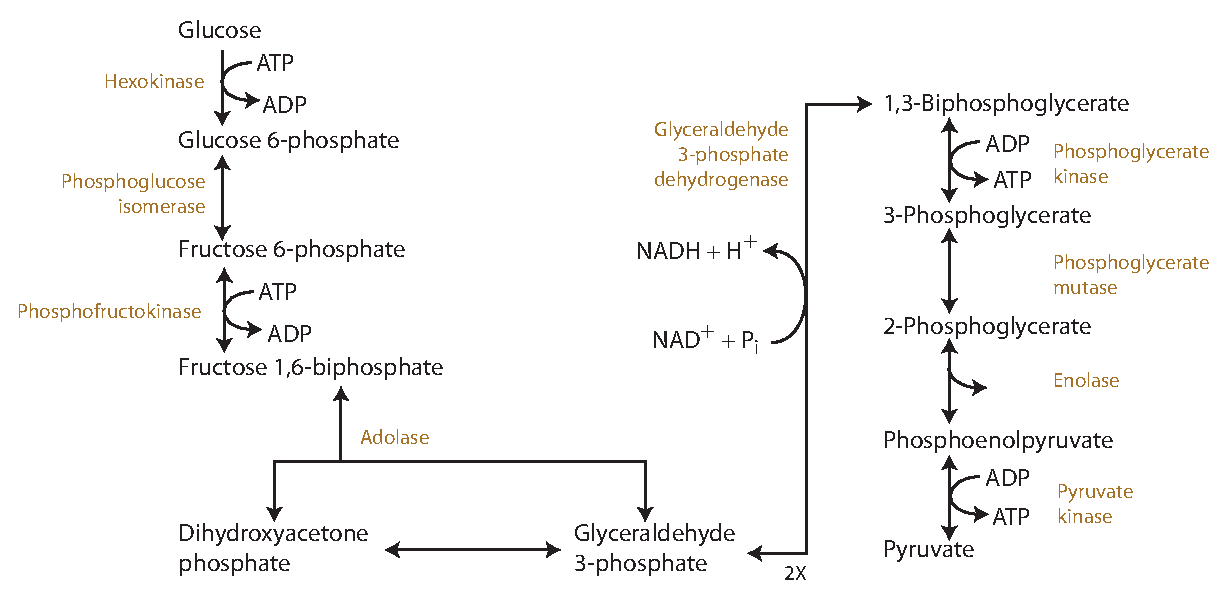
\epsfig{file=figures/glycolysis.eps, scale=0.6}
\caption{\label{fig:glycolysis}
  The glycolysis pathway. }
\end{figure}

Metabolic engineers have achieved astounding results by introducing
enzymes from one organism into others to rewrite their metabolic
pathways. For example, an enzyme from {\em Artemisia annua} (sweet
wormwood) that produces artemisinic acid was introduced into yeast
\cite{keasling-art}. Artemisinic acid is an expensive antimalarial
drug that, if it could be produced cheaply in yeast, could be very
useful in fighting malaria worldwide. However, presently it is still
not cost effective to produce this drug in yeast, mainly because
putting all of a yeast cell's resources into making artemisinic acid
makes the yeast cell unhealthy. Increasing the yields of the
artificial pathway over the past several years have involved
incredibly meticulous tuning of every step of the pathway starting
with Acetyl-CoA (one step after pyruvate) to artemisinic acid. It is
unclear how this tuning process can be automated, but if it could, the
synthesis of novel molecules in cells could become commonplace. 

\subsection{Signaling}

e.g. G-protein

\subsection{Growth and Division}

\section{Re-programming {\em E. coli}}

% how we program it (plasmids, etc)

A nice feature of {\em E. coli}, and other organisms as well, is that
an {\em E. coli} cell may contain one or more pieces of small,
circular {\em plasmid} DNA. These independently replicating pieces of
DNA are processed inside the cell much the same way as is genomic
DNA. Furthermore, it turns out to be fairly easy to construct
synthetic plasmids and stick them inside appropriately prepared
cells. Once there, the 

\section{How we See What's Going On}

% how we see what is going on: fluorescence, micrsoscopy, gene arrays,
% RT-pcr, flow-cytometry, etc. This can be brief. Perhaps a whole
% chapter can be devoted to it later.

% Regulation: Transcription factors, ribozymes and other mechanisms

% Observables: GFP, FRET, populations, single cells

% How to program cells

% Inputs: IPTG, UV, periodic inputs, etc.


\section{Problems}

\setcounter{exercount}{0}

\begin{exercise}
  An {\em E. coli} cell is an approximately 2 $\mu$m long cylinder with
  diameter 1 $\mu$m. What is its approximate volume? If there are
  about 3.6 million proteins inside a single cell, what is the
  concentration of protein in the cell in moles per liter?
\end{exercise}

\begin{exercise}
  The genetic code assigns an amino acid to each three letter sequence
  of nucleotides. How many genetic codes are possible? Why do you
  think all of the living systems (that we know of) use the same
  genetic code?
\end{exercise}

\begin{exercise}
  The molecular machinery for {\em copying} the DNA in a cell during
  cell-replication (not covered in this text) has very sophisticated
  error correction mechanisms. In contrast, the error correcting
  mechanisms for RNA polymerase (RNAP) are fairly limited -- and RNAP
  therefore makes more mistakes. Why should this be?
\end{exercise}

\begin{exercise}
  Find two different promoters in the BioBricks registry at
\begin{quote}
 \href{http://partsregistry.org/}{\tt http://partsregistry.org/}.
\end{quote}
Show the sequence of nucleotides in each and explain their
similarities and differences.
\end{exercise}



\chapter{Differential Equations}

%%
%% NOTE: This should be an appendix in the future
%%

Differential equations are the fundamental language of dynamical
systems, where they describe how quantities change with time. In
synthetic biology, the quantities of interest might be the
concentration of a particular set of proteins or metabolites or the
concentration of cells and nutrients in a solution of bacteria. When
dealing with a large number of cells, concentrations make sense and we
think of them as continuous. When dealing with single cells where
there may be only 20 of a given protein at a given time,
concentrations do not quite make sense. Nevertheless, many researchers
assume that concentrations are continuous anyway and often arrive at
useful mathematical models. 

In this chapter we look at the basic definitions, examples and
properties of ordinary differential equations. In
Chapters~\ref{ch:mak} (Mass action Kinetics) and ~\ref{ch:enzyme}
(Time Scale Separation) we describe how to derive and analyze
differential equations using modeling assumptions common in synthetic
biology.

The material given in this chapter is meant as a reminder and means to
fix notation. A much more complete introduction to differential equations
and dynamical systems requires a textbook, such as the one by Hirsch
and Smale \cite{hirsch-smale} or \cite{khalil}.

\section{Definitions and Examples}
% definitions

A system of differential equations has the form
%
\begin{eqnarray*}
\dot x_1 & = & f_1 (x_1, ..., x_n, t ) \\
         & \vdots & \\
\dot x_n & = & f_n ( x_1, ..., x_n, t )
\end{eqnarray*}
%
where $t$ is time, $x_1(t), ..., x_n(t)$ are time-dependent {\em state
  variables}, and $f_1, ..., f_n$ are functions. We usally write $x_i$
instead of $x_i(t)$. The notation $\dot x_i$ means $\frac{d}{dt}x_i$. In
vector notation, the above system is more compactly written
%
\begin{equation} \label{eqn:ode}
\dot x = f( x, t )
\end{equation}
%
where $x(t) \in \reals^n$ and $f : \reals^n \times \reals \rightarrow \reals$. 

% examples
  % bacterial growth
  % gene regulation

\begin{example} \label{ex:gene-exp} Suppose that $v_X(t)$ represents
  the concentration of a constitutively expressed protein $X$. Let the
  rate at which the protein is produced be $k_1 > 0$ and the rate at
  which it is degraded be $k_2 > 0$. Using these two parameters, a
  (very) simple model of protein production is then
%
\begin{equation}\label{eqn:gene-exp}
\dot v_X = k_1 - k_2 v_X .
\end{equation}
%
Note the term $-k_2 v_X$ describes the fact that the higher the
concentration of $X$, the more ``degradation events'' occur per
minute. The production of $X$ described by the $k_1$ term, on the
other hand, is indpendent of how much $X$ there already is in the
system. \enx
\end{example}

\begin{example} \label{ex:growth} Consider a population of of bacteria
  growing in a solution of growth media. The two variables of interest
  are the amount of bacteria $x_1$ (in grams) and the amount of nutrient
  $x_2$ (in grams) in the solution. Monod described the dynamics of this
  situation as follows \cite{monod-growth}.
\begin{eqnarray}
\dot x_1 & = & \frac{v x_1 x_2}{k+x_2} \nonumber  \\
\dot x_2 & = & - \gamma \frac{v x_1 x_2}{k+x_2} \label{eqn:monod}
\end{eqnarray}
where $v$, $k$ an $\gamma$ are parameters. Note that if $x_1=0$ or
$x_2=0$, then there is no growth since there are either no bacteria or
no nutirents. Also notice that as the nutrients $x_2 \rightarrow
\infty$, we get that the growth rate $\dot x_1 \rightarrow v
x_1$. This models the fact that the population cannot grow infinitely
quickly. The parameter $\gamma$ describes the amount of nutrients
needed to make one bacterium. Finally, the parameter $k$ describes the
{\em half-saturation} point, which is the amount of nutrient required
to make $\dot x_1 = v x_1 / 2$. \enx
\end{example}

% solutions
A {\em solution} to the differential equation \eref{eqn:ode} is an explicit
function of time $x(t)$ that satisfies the equation. Explicit
solutions are readily available for some types of differential
equations. For example, equations in which each term appears linearly
are easy to solve. However, for most differential equations, an
explicit solution is difficult or (provably) impossible to find. In
such cases, other analytical techniques must be used. 

\begin{example} \label{ex:gene-exp-sol}
The solution to linear differential equation~\eref{eqn:gene-exp} is 
%
\begin{equation}\label{eqn:gene-exp-sol}
v_X(t) = e^{-k_2 t} \left ( v_X(0) - \frac{k_1}{k_2} \right ) + \frac{k_1}{k_2}
\end{equation}
%
where $v_X(0)$ is the initial concentration of $X$. An explicit
solution such as this tells us almost everything we might want to know
about the behavior of the system. For example, it is easy to see that
as $t \rightarrow \infty$, the concentration $v_X(t) \rightarrow
k_1/k_2$.

In contrast, the differential equation~\ref{eqn:monod} is nonlinear
and has no explicit solution.  \enx
\end{example}

\section{Simulation}

Probably the first thing most analysts do with a new set of
differential equations is simulate them. There are a wide variety of
simulation tools available. For example, one can use the {\tt NDSolve} function
in Mathematica (as described in Appendix~\ref{app:math}) or the {\tt
  ode45} numerical integrator in MATLAB. All of these methods are
based on essentially the same idea. One approximates the state
$x(t+\delta)$ in some way using the state $x(t)$ and the vector field
$f(x,t)$. In this section we breifly describe a simple method of
numerically integrating a set of differential equations, called {\em
  Euler} integration. Once this method is understood, more advanced
methods should make more sense.

In Euler integration, we use the fact that
%
$$
\frac{dx}{dt} = f(x,t) = \lim_{h \rightarrow 0} \frac{x(t+h) - x(t)}{h} \approx  \frac{x(t+\delta) - x(t)}{\delta}
$$
%
when $\delta$ is small. Solving for $x(t+\delta)$ gives
%
\begin{equation}\label{eqn:euler}
x(t+\delta) \approx x(t) + \delta f(x(t),t) .
\end{equation}
%
We then have a simple algorithm.
%
\begin{enumerate}
\item initialize $x_0$, $t_0=0$ and $k=0$
\item while $t_k<t_\mathit{max}$
\item \ \ $x_{k+1} = x_k + \delta f(x_k,t_k)$
\item \ \ $t_{k+1} = t_k + \delta$
\item end while
\end{enumerate}
%
The fidelity of this approximation, and the intensity of the
compuation required, increase as $\delta$ decreases. The next example
illustrates these observations.

\begin{figure}
\epsfig{file=figures/euler.eps}
  \caption{\label{fig:euler} Simulations of bacterial growth using Euler integration
    with differing time steps. Large time steps give more results, but
    fewer steps. Smaller time give higher fidelity results.}
\end{figure}

\begin{example}
  Figure~\ref{fig:euler} shows seven simulations of the bacterial
  growth system from Example~\ref{ex:growth} with $v=2$, $k=5$,
  $\gamma=0.5$, $n(0)=10$ and $x(0)=0.1$. Note that the curves for
  $\delta=0.11$ and $\delta=0.01$ are essentially the same. Clearly
  the curves for $\delta \geq 0.21$ are of questionable fidelity. A
  large $\delta$ even introduces oscillations. \enx
\end{example}

\section{Equlibria and Stability}

% equilibria
% local stability
% stability, lyapunov

A state $x^*$ that is a root of $f$, so that $f(x^*,t) = 0$, is
called an {\em equilibrium}. A system may have zero, one or many
equilibria. Solutions to a system may tend toward $x^*$, meaning $x^*$
is stable, or they may veer away from $x^*$, meaning $x^*$ is
unstable. More formally, we are usually concerned with the following
notions of stability. 

\begin{definition} \label{def:stability}
  An equilibrium $x^*$ is {\em locally asymptotically stable} if there
  exists a $\delta>0$ such that 
$$
||x(0)-x^*|| < \delta \; \Rightarrow \; \lim_{t \rightarrow \infty} x(t) = x^* .
$$
If $\delta$ can be anything in the above, then $x^*$ is {\em globally
  asymptotically stable}. 

A system is said to be (locally or globally) {\em exponentially
  stable} if the rate of convergence to $x^*$ is exponential, that is,
if there exist constants $a,b > 0$ such that 
%
$$
||x(t)-x^*|| \leq a ||x(0)-x^*|| e^{-bt}
$$
%
for all $t \geq 0$. 
\end{definition}

\begin{example}
  Suppose that $k_1=1$ and $k_2=1$ in Example~\ref{ex:gene-exp}. The
  dynamics of $X$ are then 
%
$$
\dot v_X = 1 - v_X. 
$$
Setting the derivative equal to zero gives the equilibrium $v_X^* =
1$. As noted in Example~\ref{ex:gene-exp-sol}, the solution is 
%
$$
v_X(t) = ( v_X(0) - 1 ) e^{-t} + 1,
$$
%
which tends toward $1$ exponentially fast as $t \rightarrow
\infty$. Thus, the equilibrium $v_X^* = 1$ is globally exponentially stable. \enx
%
\end{example}

Proving that an equilibrium of a system is stable can be difficult. If
the system is linear, then it is easy. If the system in nonlinear, and
one wants to show local stability, then the system can be linearized
(see below), and the problem becomes easy. Proving that a point is
globally stable is hard, however. Also difficult is characterizing the
region (finding $\delta$ in Def.~\ref{def:stability}) around a locally
stable $x^*$ for which solutions tend toward $x^*$ (i.e. estimating
the {\em region of attraction}). Unfortunately, a point may be locally
stable with a tiny region of attraction.

% lyapunov
The main tool for proving global stability in nonlinear systems is
to use a {\em Lyapunov function}, which is an energy-like function that
decreases on all trajectories of the system as they tend toward the
equilibrium. All stable systems have Lyapunov functions, and if a
Lyapunov function can be found, the system is stable. However, find a
Lyapunov function is difficult, and no efficient method for doing so
can be found. Nevertheless, the method often proves to be useful. 

\begin{theorem} [Lyapunov's Direct Method] \label{thm:lyapunov}
  Consider a system $\dot x = f(x)$ and an equilibrium $x^*$. The
  function $V : \reals^n \rightarrow \reals$ is a {\em Lyapunov Function} if
\begin{enumerate}
\item[i.] $V(x) > 0$ for all $x \neq x^*$;
\item[ii.] $V(x^*) = 0$; and
\item[iii.] $\frac{d}{dt} V ( x ( t ) ) < 0$ for all $x \neq x^*$.
\end{enumerate}
If $V$ is a Lyapunov function, then the point $x^*$ is globally
asymptotically stable.
\end{theorem}

\begin{example} \label{ex:lyapunov}
Consider the system
%
\begin{eqnarray*}
\dot x_1 & = & x_2 \\
\dot x_2 & = & -x_1 - 2 x_2 .
\end{eqnarray*}
%
This system has an equilibrium when $x_1=x_2=0$. Now define
$V(x_1,x_2) = \frac{1}{2} ( x_1^2 + x_2^2 )$ to be a {\em candidate}
Lyapunov Function. Clearly conditions (i) and (ii) in
Theorem.~\ref{thm:lyapunov} hold. For the third condition,
%
\begin{eqnarray*}
\frac{d}{dt} V & = & \frac{d}{dt} ( x_1^2 + x_2^2 ) / 2 \\
               & = & x_1 \dot x_1 + x_2 \dot x_2 \\
               & = & x_1 x_2 + x_2 ( -x_1 - 2 x_2 ) \\
               & = & - x_2^2 < 0 
\end{eqnarray*}
%
when $x \neq 0$. We can therefore safely assume that no matter what
the initial condition, this system always converges to $0$. \enx
\end{example}

One way to visualize what at least a two-dimensional system behaves
like is to draw the vector field defined by the equations. The
resulting plot is often called a {\em phase portrait}. In particular, we
choose a number of points in the $x_1$, $x_2$ plane. For each point
$x$, we draw a vector from the point $x$ to $x + f(x)$. Since a
solution curve in the plane must be tangent to each one of these
vectors, the resulting image is quite useful.

\begin{figure}
\epsfig{file=figures/phase-lyapunov.eps}
\caption{label{fig:lyapunov} A phase portrait for the system in Example~\ref{ex:lyapunov}.}
\end{figure}

\begin{example}
  The vector field for the dynamical system in
  Example~\ref{ex:lyapunov} is shown in Figure~\ref{fig:lyapunov}. The
  stability of the point $0$ is evident.\enx
\end{example}

Besides converging to a stable equilibrium, many other limiting
behaviors are possible. A system may oscillate or it may have multiple
equilibria some of which are stable and others not. 

\begin{figure}
\begin{tabular}{cc}
\epsfig{file=figures/osc-phase.eps, scale=0.6} & \epsfig{file=figures/osc-time.eps, scale=0.8}
\end{tabular}
\caption{\label{fig:osc} (a) Phase portrait for the system in
  Example~\ref{ex:osc}. (b) The states versus time for the same system.}
\end{figure}

\begin{example} \label{ex:osc}
A phase portrait for the system
%
\begin{eqnarray*}
\dot x_1 & = & 2 x_1 - x_1 x_2 \\
\dot x_2 & = & x_1 x_2 - 2 x_2 
\end{eqnarray*}
is shown in Figure~\ref{fig:osc}. In this system, every solution in
the right-upper quadrant is periodic.
%
\end{example}

We return to the analysis of oscillations later in the book. 

\section{Linearization and Local Stability}

A powerful tool in analyzing a dynamical system is to {\em linearize}
the system around an equilibrium. Using the Taylor series, we see that
near an equilibrium $x^*$, the system
%
\begin{equation} \label{eqn:ode-not}
\dot x = f(x) 
\end{equation}
%
becomes
%
$$
\dot x = f(x) = f(x^*) + \left . \pd f x \right |_{x=x^*} (x - x^*)
       + \mathrm{higher\ order \ terms}. 
$$
The first term in the series is zero, since $x^*$ is an
equilibrium. The higher order terms are all quadratic or higher in
$x$. The second term is the linear part of $f$ near $x^*$, called the
{\em Jacobian}, and is defined by the matrix
%
\begin{equation}\label{eqn:jac}
A = \left . \pd f x \right |_{x=x^*} = \left (
\begin{array}{ccc}
\pd{f_1}{x_1}  & \dots & \pd{f_1}{x_n} \\
\vdots & & \vdots \\
\pd{f_n}{x_1} & \dots & \pd{f_n}{x_n} 
\end{array}
\right ) .
\end{equation}
%
Thus, the dynamical system $\dot x = f(x,t)$ can be approximated, near $x^*$ by
%
\begin{equation}\label{eqn:linear}
\dot x \approx A ( x - x^* ) .
\end{equation}
%
This is of great use in understanding local stability, due to the following two results. 

\begin{theorem} \label{thm:linear-to-nonlinear} If $x^*$ is an
  asymptotically stable equilibrium of \eref{eqn:linear} then it is a
  locally asymptotically stable equilibrium of \eref{eqn:ode-not}.
\end{theorem}

\begin{theorem} [Lyapunov's Indirect
  Method] \label{thm:linear-to-nonlinear} If the real parts of the
  eigenvalues of $A$ in \eref{eqn:linear} are strictly negative, then
  the point $x^*$ a stable equilibrium of \eref{eqn:linear} and a
  locally stable equilibrium of \eref{eqn:ode-not}. 
\end{theorem}

Also, if the eigenvalues of $A$ have positive real parts, you can
conclude that the equilibrium is {\em not} stable. However, if any of
the eigenvalues have zero real parts, then the method is
inconclusive. See Exercise~\ref{exer:inconclusive}. 

\begin{example}
Consider the system 
%
\begin{eqnarray*}
\dot x_1 & = & -x_1 - x_2 + x_1 x_2 \\
\dot x_2 & = & -x_2 - x_1 x_2
\end{eqnarray*}
%
This system has two equilibra, one at $0$ and the other at
$(-1,\frac{1}{2})$. The Jacobian is
%
$$
A = \left . \left ( \begin{array}{cc}
-1 + x_2 & -1 + x_1 \\
-x_2 & -1 -x_1
\end{array}
\right ) \right |_{x=x^*}
$$
%
Evaluated at the first equilibrium, $A$ is
%
$$
A_{(0,0)} = \left ( \begin{array}{cc}
-1 & -1 \\
0 & -1
\end{array} \right )
$$
%
which has eigenvalues $-1$ and $-1$. Thus, we conclude that the point
$0$ is locally asymptotically stable. Evaluated at the second point, we get
$$
A_{(-1,\frac{1}{2})} = \left ( \begin{array}{cc}
-\frac{1}{2} & -2 \\
-\frac{1}{2} & 0
\end{array} \right )
$$
which has eigenvalues $(-1 \pm \sqrt{17})/2$: one negative and the
other positive. Thus, the second equilibrium is not stable. \enx
\end{example}

\begin{example} \label{ex:chemostat} A system that is related to the
  bacterial growth system is the {\em chemostat} in which nutrients
  are pumped into the chemostat and some bacteria and depleted
  nutrients are drained out. The new nutrient mixture effectively
  dilutes the bacteria. If we call the rate of dilution $u$ (in liters
  per minute), then the equations are
%
\begin{eqnarray}
\dot x_1 & = & \frac{v x_1 x_2}{k+x_2} - u x_1\nonumber  \\
\dot x_2 & = & - \gamma \frac{v x_1 x_2}{k+x_2} + u (n_0 - x_2 ) \label{eqn:chemostat}
\end{eqnarray}
%
where $n_0$ is the number of grams of nutrient in a liter of the input
fluid. Solving for the steady state gives two equilibria. One of these
equilibria where $x_1^(=0$, meaning that the bacteria have all been
diluted away and $x_2^*$ is simply $n_0$. To examine the conditions
under which this point is a stable equilibrium, we consider the
Jacobian at this point:
%
$$
A = \left (
\begin{array}{cc}
\frac{v }n{k+n_0}-u & 0 \\
\frac{v \gamma n_0}{k+n_0} & - u
\end{array}
\right )
$$
which has eigenvalues
$$
\lambda_1 = -u \;\; \mathrm{and} \;\; \lambda_2 = \frac{v n_0}{k+n_0} - u .
$$
%
Since $u>0$, the first of these has a negative real part. For the
second to have a negative real part, we require that
%
$$
u < \frac{v n_0}{k+n_0} \defeq u_\mathrm{max}.
$$
Thus, as long as the dilution rate is less than $u_\mathrm{max}$, the
bacteria will not get simply flushed away. \enx
%
\end{example}

% Analysis of linear systems
DISCUSSION OF 2D LINEAR SYSTEMS AND EIGENVALUES GOES HERE

\section{Non-Dimensionalization}

\section{Problems}

\setcounter{exercount}{0}

\begin{exercise}
  Show that \eref{eqn:gene-exp-sol} is the solution to
  \eref{eqn:gene-exp}.
\end{exercise}

\begin{exercise} Write the equations for protein expression with RNA
  included in the model. That is suppose that some species $R$ of RNA
  is generated by a constitutively expressed gene and that $R$ is
  translated into protein $X$. Remember that both the RNA and the
  protein will degrade. Simulate your equations and compare to the
  similar model that only includes protein. 
\end{exercise}

\begin{exercise}
Find the equilibrium points of the system
%
\begin{eqnarray*}
\dot x_1 & = & \sin x_2 \\
\dot x_2 & = & \cos x_1 .
\end{eqnarray*}
%
If you understand the idea, determine the local (asymptotic) stability
of each by linearizing around each point and finding the eigenvalues.
\end{exercise}

\begin{exercise}
  (a) Show that there are an infinite number of equilibrium points of
  the bacterial growth equations in Example~\ref{ex:growth}? (a) Which
  of the equilibria are locally stable? (c) For a given initial
  condition with $x_1(0)_0$ and $x_2(0)>0$, which particular
  equilibrium point will the system go to?
\end{exercise}

\begin{exercise}
Consider the system
%
\begin{eqnarray*}
\vvec{\dot x_1}{\dot x_2} & = & \vvec{x_2(x_1+a)}{u+\sin x_1 - a x_2} \\
\end{eqnarray*}
%
Find the equilibrium points. For each equilibrium, determin conditions
on the parameter $a$ that result in stability.
\end{exercise}

\begin{exercise}
  Linearize the following system around the point $0$ to obtain a
  linear approximation and determine the local stability of the point
  $0$.
%
\begin{eqnarray*}
\dot x_1 & = & \cos ( x_2 ) - x_1 \\
\dot x_2 & = & 2 \sin ( x_1 + x_2 ) + 3 x_1 \\
\end{eqnarray*}
\end{exercise}

\begin{exercise}
  Determine the stability of the other equilibrium point in chemostat
  system of Example~\ref{ex:chemostat} when $u > u_\mathrm{max}$. 
\end{exercise}

\begin{exercise}
  Consider the system
%
\begin{eqnarray*}
\dot x_1 & = & x_2 - x_1 ( x_1^2 + x_2^2 ) \\
\dot x_2 & = & -x_1 - x_2 ( x_1^2 + x_2^2 ) .
\end{eqnarray*}
%
(a) Show that $V = x_1^2 + x_2^2$ is a Lyapunov function showing that
$0$ is globally asymtotically stable. (b) Show that Lyapunovs indirect
method is inconclusive in this case. 
%
\end{exercise}

\begin{exercise}
Simulate the system
%
\begin{eqnarray*}
\dot x & = & - y - z \\
\dot y & = & x + 0.2 y \\
\dot z & = & 0.2 + z ( x - 5.7 )
\end{eqnarray*}
from a variety of initial conditions. Show the numerical solution
curves you obtain in 3D, all in the same plot.
%
\end{exercise}

\begin{exercise}
%
Consider the function $U(x) = cos(x)$. Find the equilibria of the system
\begin{eqnarray*}
\dot x & = & -\nabla U
\end{eqnarray*}
Determine the stability of each equilibrium. Sketch the vector field and mark the basin of attraction of each equilibrium point. 
%
\end{exercise}

\begin{exercise}
%
Repeat the previous exercise, but with
\begin{eqnarray*}
\dot x & = & v \\
\dot v & = & -\nabla U - k v
\end{eqnarray*}
For what values of $k$ does this system behave like the system in the
previous exercise?
%
\end{exercise}

\begin{exercise}
%
Consider the equations
\begin{eqnarray*}
\dot x & = & \sigma(y-x) \\
\dot y & = & x(\rho-z)-y \\
\dot z & = & x y - \beta z
\end{eqnarray*}
where $\sigma = 10$, $\rho = 28$, and $\beta = \frac{8}{3}$. Use the
software of your choice to draw the flow field of this system. Since
it is three dimensional, you can either use your software to plot it
in 3D, or project the vectors into a 2D plane (such as the $x-y$)
plane. 

Next, plot two trajectories of the system, starting at very nearby
initial conditions. What happens?
%
\end{exercise}

\begin{exercise}
%
Find chemical reactions whose dynamics match the equations in the
previous exercise.
%
\end{exercise}

\chapter{Mass Action Kinetics} \label{ch:mak}

One way to describe what is going on inside a cell is to suppose that
the cell is just a very small, well-mixed test tube containing all of
the molecules (proteins, RNAs, DNAs, lipids, sugars, etc.) in a
solution of $H_2O$. That is, we ignore the unseemly reality that most
of these molecules are stuck to each other, to membranes, inside
organelles, etc. If the cell really were a test tube, then the
reactions between molecules would follow the laws of {\em mass action
  kinetics}, which we describe here. Essentially: molecules react with
each other to form new molecules at rates proportional the
concentration of the reactants.

Of course, the test tube idea is not even a remotely good assumption
about what is really happening, but it does provide us with a starting
point for modeling, and often the models obtained using mass action
kinetics are fairly informative.

Chemical kinetics is a well-estabilished area in chemistry,
mathematical modeling and non-linear systems. There are several good
sources for this material, such as the notes by Martin Feinberg
\cite{feinberg-book} from which the notes here draw heavily. Here,
however, we present the mass action kinetics using a notation
consistent with the other ideas in this book, and give examples that
are related to molecular biology rather than chemistry.

\section{Definitions}

\subsection{Reaction Networks}

In general, we name the molecular {\em species} in a system $X_1$,
$X_2$, ..., $X_N$. These might be the names of particular proteins,
messenger RNAs or small molecules. In particular examples, the species
are named with capital letters like $B$, $M$ and $E$ instead of the
generic $X_i$. A {\em reaction} among the molecular species in
question has the form
%
$$
\underbrace{n_1 X_1 + ... + n_N X_N}_\mathrm{reactants}
  \rightharpoonup \underbrace{m_1 X_1 + ... + m_N X_N}_\mathrm{products} 
$$
%
where $n_1, ..., n_N, m_1,...,m_N \in \nats \cup \{0\}$. In this
reaction, $n_i$ molecules of species $X_i$ are {\em consumed} and
$m_i$ molecules of species $X_i$ are produced. A reaction can be
written more conveniently as a vector
%
\begin{equation}\label{eqn:reaction}
a = -\vvvec{n_1}{\vdots}{n_N} + \vvvec{m_1}{\vdots}{m_N} = -a_R + a_P \in \ints^N, 
\end{equation}
%
where $a_R$ is the vector of reactant numbers and $a_P$ is the vector
of product numbers. The vector $a$ is called the {\em stoichiometry} of the reaction.

\begin{example} \label{ex:reaction} Suppose we have three species $X$, $Y$ and $Z$. The single reaction 
%
$$
X + Y \rightharpoonup Z
$$
%
can be written as a vector
%
$$
a = \vvvec{-1}{-1}{1}, 
$$
%
as long as we remember that the species are always ordered as we
presented them above. \enx
\end{example}

A system inside the cell, consisting of a number of species and the
reactions among them is modeled a {\em reaction network}, which is
simply a set of reactions. The nodes of the network are {\em
  complexes} (e.g. $X+Y$ and $Z$ in the previous example) and the
edges are the reaction arrows. Furthermore, the reaction vectors
associated with the reactions in a network can be grouped into a
matrix $A$ called the {\em stiochiometric matrix}.

\begin{example} \label{ex:network}
The reactions 
\begin{eqnarray}
X + Y & \rightharpoonup & Z \\
2Z & \rightharpoonup & X
\end{eqnarray}
%
form a reaction network with stiochiometric matrix
%
$$
A = \left ( \begin{array}{cc}
-1 & 1 \\
-1 & 0 \\
1 & -2
\end{array} \right ).
$$
%
\enx
\end{example}

\subsection{Kinetics}

In a system of reacting chemicals, the state at a particular time is
described by the {\em concentrations} of each species, usually
arranged into another vector. If $X_i$ is a species, then we write
$v_{X_i}(t)$ or just $v_i(t)$ to represent the number of molecules of
species $X_i$ per unit volume at time $t$. Then we group the
concentrations into a vector
%
$$
v = \vvvec{v_1}{\vdots}{v_n} \in \positives^N.
$$
%
It is generally assumed that the number of molecules in the
system is very large, so that stochastic effects do not come into
play. For this reason, we may call the model described in this chapter
as the {\em deterministic} model to contrast it with the {\em
  stochastic} model to be described in Chapter \ref{ch:cme}.

Associated with each reaction $a$ is a {\em reaction rate} 
%
$$
K_a : \positives^N \rightarrow \positives
$$
%
that depends on the concentrations. If $K_a(v) > 0$ then every
reactant in $a$ has nonzero concentration in the state $v$. Reaction
rates, when noted, are usually written above the reaction arrows in a
specification of the reaction. A {\em kinetics} for a network is such
an assignment of a rate to each reaction $a$. These rates may be
grouped into a vector $K(v)$ that depends on $v$:
%
$$
K(v) = \vvvec{K_{a_1}(v)}{\vdots}{K_{a_M}(v)}, 
$$
%
where we have numbered the reactions from $1$ to $M$.

The usual assumption is that the kinetics obey the {\bf law of mass
  action}, although they need not. In later chapters we will allow
the rates to be defined in other ways. For now, however, we stick with
the following definition of the rates. 

\begin{definition}
  Suppose that $a$ is defined as in \eref{eqn:reaction}. Then the
  {\em mass action rate} for the reaction $a$ os definted by
%
\begin{equation}\label{eqn:mak-rate}
K_a(v) \defeq k_a \prod_{i}v_i^{n_i}
\end{equation}
%
where $k_a$ is called the {\em rate constant} for the reaction
$a$. 
\end{definition}

The idea the following. Suppose that an $X$ molecule reacts with
a $Y$ molecule according to the reacton
%
$$
X + Y \xrightharpoon[\text{}]{\text{$k$}} Z
$$
%
If there are $v_X$ molecules of type $X$ per liter and $v_Y$ molecules
of type $Y$ per liter, then the number of possible reactions that can
occur per liter is $v_X v_Y$. Since some types of reactions may be
stronger or faster than others, we add a rate constaint $k$ to our
model to obtain $kv_Xv_Y$. When the rate constant is important, we
make a note of it by writing it, as above, near the arrow used to
specify the reaction.  The definition \eref{eqn:mak-rate} is a
generalization of the idea of having the rate of a reaction include a
term that desribes the number of ways that a reaction can happen: the
rate is proporional to the current concentrations, or masses, of the
reactants.

\begin{example} \label{ex:mak}
The reaction rates for the reactions in Example~\ref{ex:network} are
$$
K(v) = \vvec{k_1 v_X v_Y}{k_2 v_Z^2}
$$
%
where we suppose that $k_1$ and $k_2$ are the rate constants for the two reactions in
the network respectively. \enx
\end{example}

\subsection{The Determinstic Equations}

The rate at which the concentrations in a reaction network change
leads to a set of differential equations, called the deterministic
equations (to contrast them with the stochastic equations we study
later) that can be written succinctly as
%
\begin{equation} \label{eqn:mak}
\dot v = A K(v) .
\end{equation}
%
Along with an initial concentration vector $v(0)$ and actual values
for the rate constants, this completely specifes the behavior of a
reaction network.

\begin{example} Applying  \eref{eqn:mak} to the stoichiometric matrix $A$ in
  Example~\ref{ex:network} and the rate vector $K(v)$ in
  Example~\ref{ex:mak} gives
%
$$
\vvvec{\dot v_X}{\dot v_Y}{\dot v_Z} = A K(v) 
  = \vvvec{-k_1 v_X v_Y + k_2 v_Z^2}{-k_1 v_X v_Y}{k_1 v_X v_Y - 2 k_2 v_Z} ,
$$
%
which is simply a list of three equations stating how the
concentrations of $X$, $Y$ and $Z$ in the network change over time. \enx
\end{example}

\subsection{Basic Properties}

The mass action kinetics equations for a given network are, in
general, nonlinear. Explicit, closed-form solutions for the equations
do not exist except in simple situations. However, systems of
differential equations arising from mass action kinetics are not
entirely arbitrary either, and all mass action systems obey some
simple properties, which we now discuss.

The first property states that concentrations can never be negative as
long as they start out positive. This property is certianly true of
actual physical systems. Mathematically, the property holds because if
a concentration ever becomes zero, its rate of change is necessarily
non-negative.

\begin{property} \label{prop:nonneg} If $v \in \positives$ and
  $v_i=0$, then $\dot v_i \geq 0$.
\end{property}

\begin{proof}
  Every reaction $a$ in which $X_i$ shows up as a reactant has $K_a(v)=0$
  whenever $K_a(v)$ is defined by Equation~\eref{eqn:mak}. Thus 
  contributions to $\dot v_i$ are only from reactions in which $X_i$
  appears as a {\em product} and are therefore non-negative. 
\end{proof}

The next property describes the set of all possible concentration
vectors that can be reached starting from a given initial
condition. We first require a definition:

\begin{definition}\label{def:stoich-sub}
The {\em stoichiometric subspace} of a system with matrix $A = (a_1,...,a_N)$ is
%
\begin{eqnarray*}
S & = & \mathrm{span} A = \mathrm{span} \{ a_1, ..., a_N \} \\
  & = & \{ r_1 a_1 + ... + r_N a_N \;|\; r_1, ..., r_N \in \reals \}. 
\end{eqnarray*}
The {\em rank} of a reaction network is the rank of $S$ (i.e. the
number of linearly independent columns or rows). If $v_1-v_2 \in S$,
then $v_1$ and $v_2$ are said to be {\em stoichiometrically
  equivalent}.
%
\end{definition}

\begin{example} \label{ex:span}
Suppose that
$$
A = \left ( \begin{array}{cc}
-1 & 1 \\
-1 & 0 \\
1 & -2
\end{array} \right ).
$$
as in Example~\ref{ex:network}. Then
%
$$
S = \left \{ \vvvec{r_2-r_1}{-r_1}{r_1-2r_2} \;|\; r_1,r_2 \in \reals \right \}. 
$$
%
In this case, $S$ is a two dimensional subspace of $\reals^3$, suggesting
that the three differential equations we use to describe it are
redundant in some way. \enx
\end{example}

The notion of {\em stiochiometrically equivalent} leads to equivalence
classes of states and the simple property that all solutions of a mass
acton kinetics system remain in an equivalence class defined by the
initial condition. This is characterized in the following property.

\begin{property} \label{prop:equiv}
All solutions $v(t)$ of 
%
$$
\dot v = A K(v) \;\;\;\;\; \mathrm{with} \; v(0) \; \mathrm{given}
$$
%
lie in the stochiometric equivalence class of $v(0)$. I.e. $v(t)$ is
always stoichiometrically equivalent to $v(0)$. 
\end{property}

\begin{proof} The property follows from the definition of the
  derivative and of $S$:
$$\dot v = \lim_{h \rightarrow 0} \frac{v(t+h)-v(t)}{h} = A K(v) \in S.$$
\end{proof}

These notions can be best seen in a two-dimensional example.

\begin{example} \label{ex:stoich}
Consider the network
%
$$
X \xrightleftharpoons[\text{$k_2$}]{\text{$k_1$}} 2 Y 
$$
%
with the initial condition defined by $v_X(0)=1$ an $v_Y(0)=0$. The
stiochiometric matrix is
%
$$
A = \left ( \begin{array}{cc}
-1 & 1 \\
2 & -2
\end{array} \right )
$$
%
and
%%
$$
S = \left \{ \vvec{-r}{2r} \;|\; r \in \reals \right \}. 
$$
%%
By Property \ref{prop:equiv}, for every $t$ there exists an $r$ such that
%
$$
v(t) - v(0) = \vvec{v_X(t)}{v_Y(t)} - \vvec{1}{0} = \vvec{-r}{2r}
$$
%
from which it follows that all $v(t)$ have form
%
$$
\vvec{1-r}{2r} .
$$
%
Furthermore, since all concentrations must be non-negative, $r \in
[0,1]$. We can further analyze this system be looking at the locus of
equilibra. Setting
%%
$$
\dot v = A K(v) = \vvec{-k_1 v_X + k_2 v_Y^2}{k_1 v_X - k_2 v_Y^2} = 0,
$$
%%
we get $k_1 v_X = k_2 v_Y^2$ or $v_X = \frac{k_2}{k_1} v_Y^2$. The
general picture is shown in Figure~\ref{fig:stoich}. 
\end{example}

\begin{example}
  Continuing with the previous example, we note that the system is
  really one dimensional. We can write it in terms of $r$ in fact as
  follows:
%
\begin{eqnarray*}
\dot r & = & \frac{\dot v_Y}{2} \\
       & = & \frac{1}{2} \left ( k_1 v_X - k_2 v_Y^2 \right ) \\
       & = & \frac{1}{2} \left ( k_1 (1-r) - k_2 (2r)^2 \right ) \\
       & = & \frac{k_1}{2}(1-r) - 4 k_2 r^2 .
\end{eqnarray*}
%
Anything true abut this equation can be translated back to statements
about the original set of equations. \enx
\end{example}

\begin{figure}

\epsfig{file=figures/stoich-sub.eps}

  \caption{\label{fig:stoich} The stoichiometric subspace from
    Example~\ref{ex:stoich} is a one-dimensional line connecting
    $(1,0)$ to $(0,2)$. The points on this line tend toward the point
    where stoichiometric subspace intersects the locus of equilibra}

\end{figure}

\section{Example Networks}

\subsection{Sources and Sinks}

If $a_r = 0$, then the species in $a_p$ appear from nowhere. Thus,
$a_r=0$ models a {\em source}. We write, equivalently,
%
$$
0 \rightharpoonup a_p
$$
%
and 
%
$$
\varnothing \rightharpoonup m_1 X_1 + ... + m_N X_N .
$$
%
Similarly, if $a_p = 0$, then reactants can disappear from the system
and $a_p=0$ is called a {\em sink}. 

\begin{example}
The reaction 
%
$$
\varnothing \xrightharpoon[\text{}]{\text{$k$}} A
$$
%
has the mass action kinetics
%
$$
\dot v_A = k.
$$
%
That is, $A$ is added to the system at a constant rate.
\enx
\end{example}

\begin{example}
The reaction 
%
$$
A \xrightharpoon[\text{}]{\text{$k$}} \varnothing 
$$
%
has the mass action kinetics
%
$$
\dot v_A = - k v_A.
$$
%
That is, the more $A$ is in the system, the faster its concentration
decreases. \enx
\end{example}

\subsection{Constant Concentrations}

In the cell, many species are regulated using feedback so that they
maintain essentially constant levels. For example, ATP -- the basic
unit of energy -- is regulated tightly \cite{ATP_IS_REGULATED}. ATP is
also involved in many reactions. We could include ATP as a reactant or
product in all of the reactions in our network, but because it is
regulated, we would also have to include the regulation machinery in
our model as well. To get around this, we usually just pretend that
$\dot v_{ATP}=0$ and write, for example,
%
$$
X  \xrightharpoon[\text{}]{\text{$k v_{ATP}$}} Y
$$
%
to denote that the rate at which $X$ is converted into $Y$ depends on
the concentration of $ATP$. The above reaction gives the kinetics
%
$$
\dot v_X = - \dot v_Y = - k v_{ATP} v_X 
$$
%
where $v_{ATP}$ does not depend on time (i.e. it is a constant
parameter in our model). 

\subsection{Membranes}

Say $X$ and $Y$ react according to the reaction
%
$$
X  \xrightleftharpoons[\text{$k_2$}]{\text{$k_1$}} 2 Y 
$$
%
in two compartments separated by a membrane with some active transport
mechanism across it, as in Figure~\ref{fig:membrane}. To model this
system with mass action kinetics, we define new symbols $X_1$ and
$X_2$ to refer to $X$ molecules when they are in compartent one and
compartment two, respectively. Similarly, we introduce the names $Y_1$
and $Y_2$. We can the write the reaction network

\begin{center}
\begin{tabular}{ccc}
$X_1  \xrightleftharpoons[\text{$k_2$}]{\text{$k_1$}} 2 Y_1$ & \ \ \ \ \ & $X_1  \xrightleftharpoons[\text{$k_4$}]{\text{$k_3$}} X_2$ \\
\ & \ & \\
$X_2  \xrightleftharpoons[\text{$k_2$}]{\text{$k_1$}} 2 Y_2$ & \ \ \ \ \ & $Y_1  \xrightleftharpoons[\text{$k_6$}]{\text{$k_5$}} Y_2$ 
\end{tabular}
\end{center}

\noindent
which describes a system with four ``species'' that model our two
species reacting in a two-compartment system.

\subsection{Conservative Systems}

For the system 
%
$$
X  \xrightleftharpoons[\text{$k_2$}]{\text{$k_1$}} 2 Y 
$$
%
we can define a vector $m$ by
%
$$
m = \vvec{2}{1}
$$
%
and note that
%%
\begin{eqnarray*}
\frac{d}{dt} m^T v & = & m^T \dot v = m^T A K(v) \\
 & = & (2 \; 1) {\left ( \begin{array}{cc} 
  -1 & 1 \\
  2  & -1 \end{array} \right ) K(v) } \\
 &   & \\
 & = & ( 0 \; 0 ) K(v) = 0 .
\end{eqnarray*}
%%
The idea is that $X$ molecules have twice the mass of $Y$ molecules
and $m$ records this fact. The quantity $m^Tv$ is the total mass of
the system over all species. Its derivative is zero because mass in
conserved in this system. 

In contrast, the system
%
$$
X  \xrightharpoon[\text{}]{\text{$k_1$}} 2 Y 
$$
%
$$
Y  \xrightharpoon[\text{}]{\text{$k_2$}} X
$$
%
where $Y$ decays back into a single $X$ (forgetting that it seems to
have been constructed out of two $X$ molecules) does not have a
meaningful mass vector. This is because
%
$$
m^T A = ( m_X \; m_Y ) \left ( \begin{array}{cc} 
  -1 & 1 \\
  2  & -1 \end{array} \right ) = \vvec{0}{0}
$$
%
has no non-trivial solution. In this case, the network is not conservative. 

Another possibility is that $m^TA=0$ may have no positive solution. A
negative solution would lead to a strange definition of mass. These
ideas motivate the following definition. First, recall that if we are
given a subspace $S$ of a vector space $V$, the {\em orthogonal
  compliment} of $S$ is 
%
$$
S^\bot = \{ u \in V \;|\; u^Tv = 0, \; \forall v \in S \} . 
$$

\begin{definition} \label{def:conservative} A reaction network with
  stoichiometric subspace $S$ is conservative if there is a positive
  vector $m$ contained in $S^\bot$. 
\end{definition}

To find a mass vector, then, one has to solve $m^TA$ for $m$ and see
if $m$ can be positive. This amounts to solving a system of linear
equations, which can be done with Gaussian elimnation, for example.

\begin{figure}
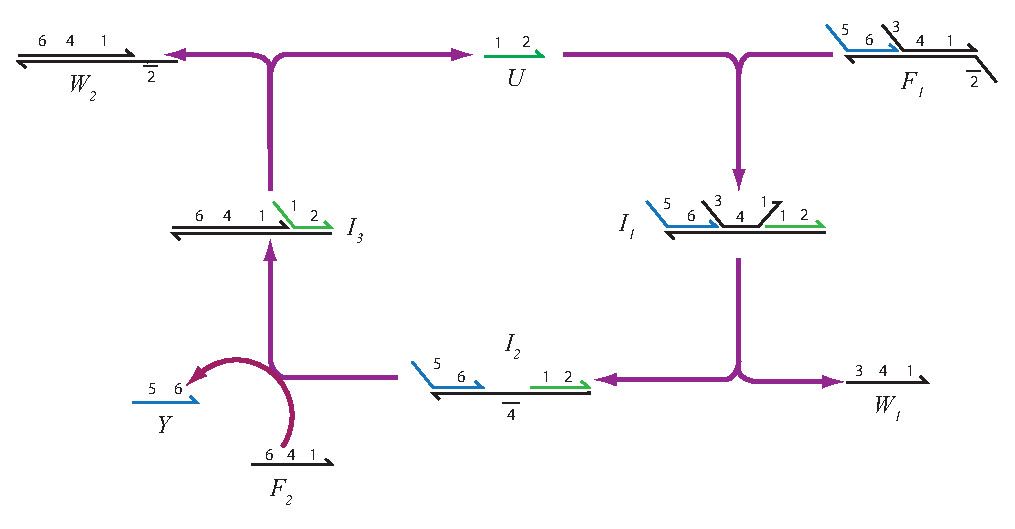
\epsfig{file=figures/zhang-integrator.eps, scale=0.75}
\caption{\label{fig:zhang-integrator} A DNA hybridization circuit from
  \cite{zhang-integrator}. Each line represents a single stranded
  piece of DNA. Parallel lines correspond to double stranded
  DNA. Numbers denote binding domains, which are unique seqnences of
  A, T, C or G nucleotides. A number with a bar denotes a
  complimentary sequence.}
\end{figure}

\begin{example}\label{ex:zhang-integrator}
  Consider the network in Figure~\ref{fig:zhang-integrator}. In it,
  oligonucleotides form and unform complexes of one or more
  oligos. Thus each complex is a species, but it is also made up of
  individual oligos, suggesting that the number of oligos in a complex
  should be the mass of the complex. For this system, we have the
  following reactions (ignoring the rates for now).
%
\begin{eqnarray*}
U + F_1 & \rightharpoonup & I_1 \\
I_1 & \rightharpoonup & W_1 + I_2 \\
I_2 + F_2 & \rightharpoonup & I_3 + Y \\
I_3 & \rightharpoonup & W_2 + U .
\end{eqnarray*}
%
If we define $v = ( U \; F_1 \; F_2 \; I_1 \; I_2 \; I_3 \; W_1 \; W_2 \; Y )^T$
then a suitable mass vector is
%
$$
m = ( 1 \; 3 \; 1 \; 4 \; 3 \; 3 \; 1 \; 2 \; 1 ) ,
$$
%
where the mass of each species is given by the number of oligos in
it. This fact is confirmed in an exercise.  \enx
\end{example}

\section{Modeling Regulatory Networks and Metabolism}

% Put a bunch of snippets of GRNs and 
%
% start with a single gene
% then a gene with a repressor
% then one with an activator
% then one with some protein-protein intreaction, like in the ARF system
%

% A <-> B -> C : Show that increasing forward and reverse rate of first 
% reaction 

In this section we explore how mass action kinetics can be used to
model genetic regulatory networks and metabolism. We start by modeling
a single gene, and then simple combinations of genes. Finally, we show
an example from metabolism. In the next chapter we show how the
systems here can be simplified to some extent using a set of
approximation called {\em enzyme kinetics}. 

\begin{example} \label{ex:onegene}
  Consider a single consitutively expressed gene producing a single
  protein $X$ at a rate $k_1$. The protein is degraded and diluted due
  to cell growth at a rate $k_2$. Note that the concentration of RNAP,
  like ATP above, is regulated and, therefore, does not appear in
  these reactions. Instead it is absorbed into the rate constant
  $k_1$. Similarly, the concentration of proteins that degrade protein
  is absorbed into $k_2$. A simple model of our system is then
%
$$
\varnothing \xrightharpoon[\text{}]{\text{$k_1$}} X \xrightharpoon[\text{}]{\text{$k_2$}} \varnothing
$$
%
which gives the differential equation
%
$$
\dot v_X = k_1 - k_2 v_X.
$$
%
A more sophisticated model of this system includes the messenger RNA
intermediate. Let's call it $R$. The gene produces $R$ and $R$
produces proteins before being degraded and
diluted. Adding these complexities to our model gives
%
$$
\varnothing \xrightharpoon[\text{}]{\text{$\kappa_1$}} R \xrightharpoon[\text{}]{\text{$\kappa_2$}} \varnothing
$$
%
%
$$
R \xrightharpoon[\text{}]{\text{$\kappa_3$}} R + P 
$$
%
%
$$
P \xrightharpoon[\text{}]{\text{$\kappa_4$}} \varnothing
$$
%
The second line, where $R$ produces $P$ shows that the mRNA is not
consumed in the process of being transcribed into protein. Note also
that the concentration of ribosomes is absorbed into $\kappa_3$. 
The above system gives rise to the equations
%
\begin{eqnarray*}
\dot v_R & = & \kappa_1 - \kappa_2 v_R \\
\dot v_P & = & \kappa_3 v_R - \kappa_4 v_P .
\end{eqnarray*}
%
One might ask: {\em What values of $k_i$ and $\kappa_i$ make these two
  descriptions similar?} To answer this, note that the rate of
production and degradation of mRNA is faster than with protein. Thus,
we can assume that the level of mRNA equilibrates quickly, meaning that
%
$$
\dot v_R = \kappa_1 - \kappa_2 v_R = 0
$$
%
which implies that $R = \kappa_1/\kappa_2$ fairly soon. Thus, the
equation for protein production becomes
%
$$
\dot v_P = \kappa_3 \frac{\kappa_1}{\kappa_2} v_R - \kappa_4 v_P .
$$
This implies that 
%
$$
k_1 = \frac{\kappa_3\kappa_1}{\kappa_2} \;\;\;\mathrm{and} \;\;\; k_2 = \kappa_4 . 
$$
%
A simulation of these two systems is shown if
Figure~\ref{fig:onegene}. Note that the main difference in the two
curves is that initially, $\dot v_P = 0$ in the more complex
model. This may be an insignificant difference in some situations, but
in others in is crucially important (as in Example~\ref{ex:repressilator}). 
\enx
\end{example}

\begin{figure}
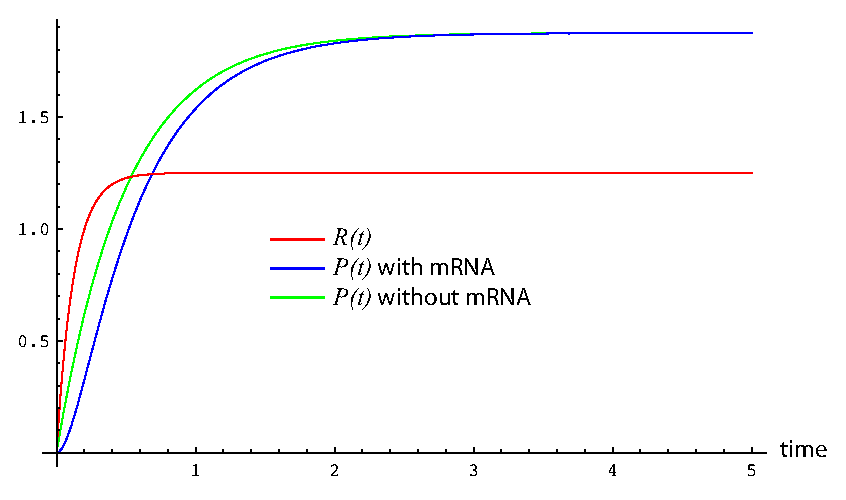
\epsfig{file=figures/one_gene.eps, scale=0.7}
\caption{\label{fig:onegene}
Two models of gene expression, one modeling mRNA explicitly and the other not. 
}
\end{figure}

\begin{example} \label{ex:repression}
  Now consider a gene $g$ that produces a protein product $X$ that is
  repressed by a transcription factor $T$. In reactions, this can be written
%%
$$
g \xrightharpoon[\text{}]{\text{$k_1$}} g + P 
$$
$$
P \xrightharpoon[\text{}]{\text{$k_2$}} \varnothing
$$
$$
T + g \xrightleftharpoons[\text{\text{$k_4$}}]{\text{$k_3$}} g_\mathrm{off} .
$$
%%
The first reaction models the fact that the gene $g$ produces a
protein product $P$ at some rate, without itself being consumed. The
second reaction models protein degradation. The third line models the
interaction between the transcription factor $T$ and the gene
$g$. When $T$ is bound to $g$, RNAP is unable to bind to $g$ to
produce $P$, thus the name $g_\mathrm{off}$. Note that there is a
conservation of mass with $g$ and $g_\mathrm{off}$. Namely, there is
some constant $C$ such that
%
$$
v_g + v_{g_\mathrm{off}} = C.
$$
%

We now consider the steady state concentration of $P$ for varying
input concentrations of $T$. Since
$$
\dot v_P = k_1 v_g - k_2 v_P, 
$$
we have $v_P^* = k_1 v_g^* / k_2$. The dynamics of $g$ are given by
$$
\dot v_g = -k_3 v_T v_g + k_4 ( C - v_g ) 
$$
so that
$$
v_g^* = \frac{k_4  C}{k_3 v_T + k_4} . 
$$
Thus, by substituting the above into the equation for the steady state
concentration of $P$, we can see it is inversely related to the
concentration of $T$:
$$
v_P^* = \frac{k_1 k_4  C}{k_2 k_3 v_T + k_2 k_4} . 
$$
In the next chapter we study these kinds of relationships more extensively.
\enx
\end{example}

\begin{example} \label{ex:repressilator}
The repressilator.
\end{example}

\begin{example}
Relaxation oscillator.
\end{example}



\section{Problems}

\setcounter{exercount}{0}

\begin{exercise} Find the stable equilibrium in Example~\ref{ex:span}
  assuming $k_1=k_2=1$.\end{exercise}

\begin{exercise} The system in Example~\ref{ex:network} is really
  two-dimensional. Write the equations in terms of $\dot r_1$ and
  $\dot r_2$ to show this.\end{exercise}

\begin{exercise} Confirm that $m$ defined in Example~\ref{ex:zhang-integrator} is
  indeed a mass vector by writing the stiochiometric matrix for the
  system and pre-multiplying it by $m$. \end{exercise}

\begin{exercise}
Consider ther system
%%
$$
2X+Y \xrightharpoon[\text{}]{\text{$1$}} X+2Y .
$$
%%
\begin{enumerate}
\item[a)] Find the stoichiometric matrix $A$ and the kinetics vector
  $K(\vec v)$. Use these to find the mass action equations.
\item [b)] Find the stochiometric subspace and its dimension.
\item [c)] Pick a reasonable initial condition and describe its
  stoichiometric equivalence class.
\item [d)] If the system is conservative, determine a mass vector. Or
  state why the system is not conservative.
\item [e)] Determine the equilibrium points of the network, the
  Jacobians evaluated at these points, and the stability of the
  points.
\item [f)] Draw a vector flow field for the network.
\end{enumerate}
\end{exercise}

\begin{exercise}
Repeat the steps in  for the following network
\begin{eqnarray*}
X & \xrightharpoon[\text{}]{\text{$1$}} & 2X \\
X+Y & \xrightharpoon[\text{}]{\text{$1$}} & 2Y \\ 
Y & \xrightharpoon[\text{}]{\text{$2$}} & \varnothing .
\end{eqnarray*}
\end{exercise}

\begin{exercise}
  Show that the two models of protein production from a single gene in
  Example~\ref{ex:onegene} give the same steady state amount of
  protein.
\end{exercise}

\begin{exercise}
Consider the system
%%
$$
\varnothing \xrightleftharpoons[\text{\text{$1$}}]{\text{$1$}} X  \xrightharpoon[\text{}]{\text{$3$}} Y
$$
$$
2X+Y \xrightharpoon[\text{}]{\text{$1$}} 3 X .
$$
Find the equilibria and determine their local stability. What do the
imaginary parts of the eigenvalues mean? Simulate the system from a
variey of initial conditions and describe the behavior obtained.
%%
\end{exercise}


\chapter{Enzyme Kinetics} \label{ch:enzyme}

\section{Fast and Slow Dynamics}

Suppose we are modeling a system in which some states, call them $z$
more very quickly to some equilibrium value. Meanwhile other states,
call them $x$, change more slowly. In equations, we write
%
\begin{eqnarray}
\dot x & = & f ( x, z, t, \epsilon ) \label{eqn:fast-slow1} \\
\epsilon z & = & g ( x, z, t, \epsilon ). \label{eqn:fast-slow2}
\end{eqnarray}
%
Here, $\epsilon$ denotes some system parameter (such as a reaction
rate), that is very small compared with other parameters. You can see
that if you divide \eref{eqn:fast-slow2} by $\epsilon$ then the rate
of change of $z$ is, thus, large. 

Since $\epsilon$ is small, we might as well ask what if
$\epsilon=0$. In this case, \eref{eqn:fast-slow2} becomes
%
\begin{equation} \label{eqn:fast-slow-eqality}
g ( x, z, t, 0 ) = 0. 
\end{equation}
%
Suppose that $z=h(x,t)$ is a solution to
\eref{eqn:fast-slow-equality}. Then the ``slow dynamics'' of $x$ are
described by
%
\begin{equation} \label{eqn:fast-slow-reduced}
\dot x = f ( x, h(t,x), t, 0 ), 
\end{equation}
%
that is, solely in terms of $x$. Thus, by assuming that $\epsilon=0$,
we have come up with a reduced model of the original system. It turns
out that how much smaller $\epsilon$ is compared to other parameters
in the system determines the degree to which the full and reduced
models are similar.

\section{Enzyme Reactions}

\subsection{The Michaelis-Menten Model}

As an example, consider the reaction
%
$$
E + S \xrightleftharpoons[\text{$k_2$}]{\text{$k_1$}} ES \xrightharpoon[\text{}]{\text{$k_3$}} E + P
$$
%
which describes how a species of enzyme $E$ interacts with a substrate
species $S$ to produce a product species $P$. An enzyme molecule may repeatedly
bind to substrate molecules to form enzyme-substrate complexes
$ES$. Eventually the enzyme turns the a substrate molecule into a
product. It is often the case that
$$
k_1, k_2 \gg k_3, 
$$
suggesting that the population of $ES$ stabilizes quickly compared to
the production of $P$. 

\begin{figure}
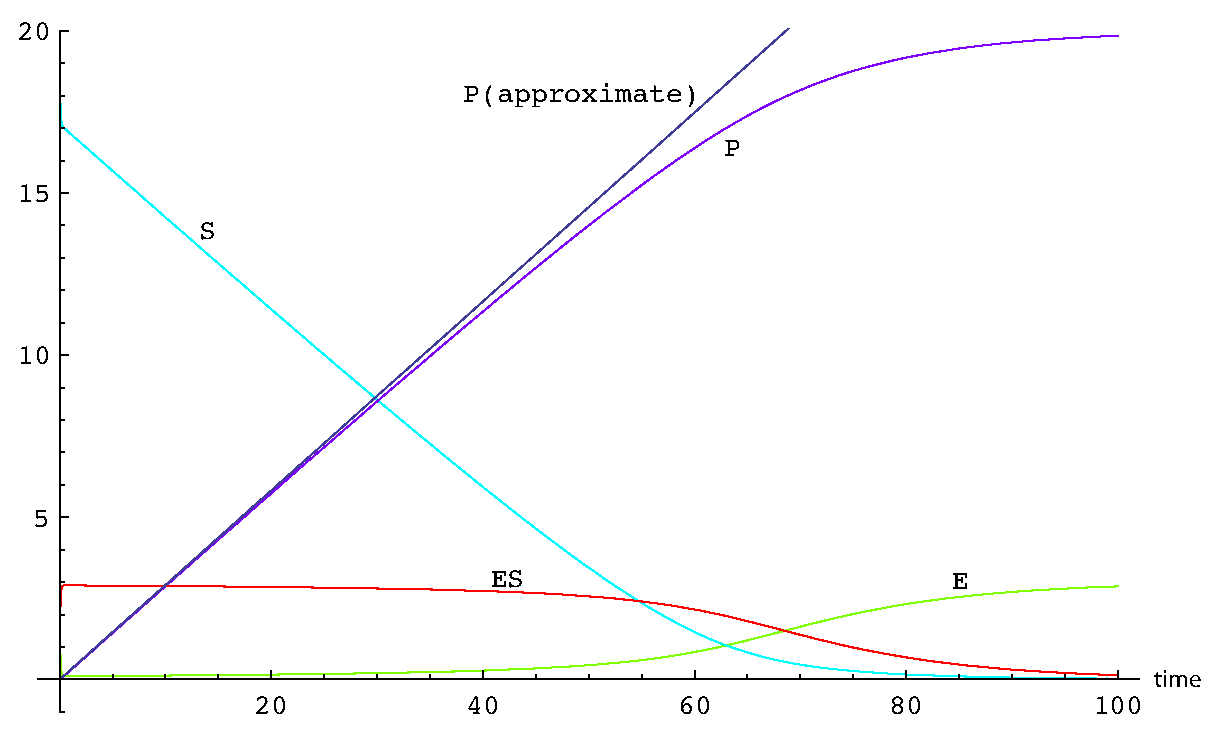
\epsfig{file=figures/michaelis-menton.eps, scale=0.6}
  \caption{\label{fig:mm} The simple enzyme substrate reaction and the
    Michaelis-Menton approximation. Here, $k_1=1.0$, $k_2=0.5$,
    $k_3=0.1$, $v_E(0)=3$ and $v_S(0)=20$.}
\end{figure}

Now consider the analysis question: at approximately what rate is $P$
produced, ignoring the brief period of time during which $ES$ is
equilibrating? Treating $v_S$ as a constant (i.e. assuming there are a
very large number of substrate molecules), and using the law of mass
action gives
\begin{eqnarray}
\dot v_{P}  & = & k_3 v_{ES} \\
\dot v_{ES} & = & k_1 v_E v_s - k_2 v_{ES} - k_3 v_{ES} .
\end{eqnarray}
The total amount of enzyme does not change so that $v_E + v_{ES} =
E_{tot}$. Thus, the equation for $\dot v_E$ is not needed and
%
\begin{eqnarray*}
\dot v_{ES} & = & k_1 (E_{tot}-v_{ES}) v_s - k_2 v_{ES} - k_3 v_{ES} \\
           & = & k_1 e_{tot} v_s - (k_1 s + k_2 + k_3 ) v_{es} .
\end{eqnarray*}
%
Now define $\epsilon \defeq (k_1 v_s + k_2 + k_3)^{-1}$. By our assumptions
on the relative magnitudes of the $k_i$ and that $s$ is large, it
follows that $\epsilon$ is small. We can now write:
%
\begin{eqnarray}
\dot v_{P}  & = & k_3 v_{ES} \label{eqn:mm-sv1} \\
\epsilon \dot v_{ES} & = & \frac{k_1 e_{tot} v_s}{k_1 v_s + k_2 + k_3} - v_{es},  \label{eqn:mm-svp2}
\end{eqnarray}
%
which matches \eref{eqn:fast-slow1} and \eref{eqn:fast-slow2}. Setting
the fast dynamics to zero gives the constraint that
%
$$
v_{es} = \frac{k_1 e_{tot} v_s}{k_1 s + k_2 + k_3}
$$
%
and substituting into \eref{eqn:mm-sv1} gives
%
$$
\dot v_{P} = \frac{k_3 k_1 e_{tot} v_s}{k_1 v_s + k_2 + k_3} = \frac{k_3 e_{tot} v_s}{v_s + \frac{k_2+k_3}{k_1}}.
$$
Chemists and biologists like to define
%
$$
V_{max} \defeq k_3 e_{tot} \;\;\;\;\; K_m = \frac{k_2+k_3}{k_1}
$$
%
so that we arrive at the {\em Michaelis-Menton} model:
%
\begin{equation} \label{eqn:mm}
\dot v_{P} = \frac{V_{max} v_s}{v_s+K_m}.
\end{equation}
%
The constant $V_{max}$ is commonly referred to as the maximum
production rate, which you get when $v_s \rightarrow \infty$. The
constant $K_m$ is called the half saturation constant, which is the
concentration of $S$ required to get a rate of $V_{max}/2$. 

The situation is shown in Figure~\ref{fig:mm}. Initially, while the
amount of substrate is high, the rate of change of $P$ is essentially
constant with slope defined by Equation~\eref{eqn:mm}. Eventually, the
substrate is depleted, and the assumption that $\dot v_S = 0$ no
longer holds.

\subsection{Competetive Inhibition}

Now consider a system consisting of an enzyme in one of two states,
either active $E$ or bound to a deactivator $I$ to form an inactive
complex $EI$. The reactions are
$$
E + S \xrightleftharpoons[\text{$k_{-1}$}]{\text{$k_1$}} ES \xrightharpoon[\text{}]{\text{$k_2$}} E + P
$$
$$
E + I \xrightleftharpoons[\text{$k_{-3}$}]{\text{$k_3$}} EI .
$$
In this case, we say that $I$ and $S$ are in competition for $E$. If
$ES$ and $EI$ equilibrate quickly, then it seems reasonable to
approximate the system by a simple one dimensional system in which the
product $P$ is produced at some rate that is a function of the
concentrations of $S$ (which we'll assume is large and relatively
unchanging) and $I$ (which is not produced or consumed). 

First, note that there we have the conservation constraint that the
enzyme is either free, bound to an $S$ or bount to an $I$. That is, 
%%
$$
v_{tot} = v_E + v_{ES} + v_{EI}. 
$$
%%
Assuming that $ES$ and $EI$ equilibrate quickly gives
$$
\dot v_{ES} = 0 = k_1 v_E v_S - (k_{-1}+k_2)v_{ES}
$$
%%
so that $v_Ev_S = K_m v_{ES}$ where $K_m = ( k_{-1}+k_2 ) / k_1$ and
$$
\dot v_{EI} = 0 = k_3 v_E v_I - k_{-3} v_{EI}
$$
which implies that $v_E v_I = K_3 v_{EI}$ where $K_3 =
\frac{k_{-3}}{k_{3}}$. Putting these relationships into the constraint
above gives
%
\begin{eqnarray*}
v_{tot} & = & \frac{K_m v_{ES}}{v_S} + \frac{v_Ev_I}{K_3} + v_{ES} \\
       & = & \frac{K_mv_{ES}}{v_S} + \frac{K_mv_{ES}}{v_S} \frac{v_I}{K_3} + v_{ES}
\end{eqnarray*}
%
which implies that 
%
$$
v_{ES} = \frac{v_{tot}}{\frac{\displaystyle K_m}{\displaystyle v_S} + \frac{\displaystyle K_m v_I}{\displaystyle K_3v_S} + 1}
       = \frac{v_{tot}v_S}{K_m + \frac{\displaystyle K_m}{\displaystyle K_3}v_I + v_S} .
$$
%
From the above expression for $v_{ES}$ it follows that
%
\begin{equation}
\dot v_P \approx \frac{V_{max} v_S}{K_m + \frac{\displaystyle K_m}{\displaystyle K_3} v_I + v_S}
\end{equation}
%%
where 
%%
$$
V_{max} = k_2 v_{tot} \;\;\;\; K_m = \frac{k_{-1}+k_2}{k_3} \;\;\;\; \mathrm{and} \;\;\; K_3 = \frac{k_{-3}}{k_3}. 
$$
If there is no inhibitor $I$, we get the same results as with the
Michaelis-Menton system. As the concentration of $I$ increases, the
rate of production of $P$ goes to zero. Finally, if there is a high
concentration of $S$, then $\dot v_P \approx V_{max}$. The situation
is shown in Figure~\ref{fig:comp-inhibit} \enx
%%

\begin{figure}
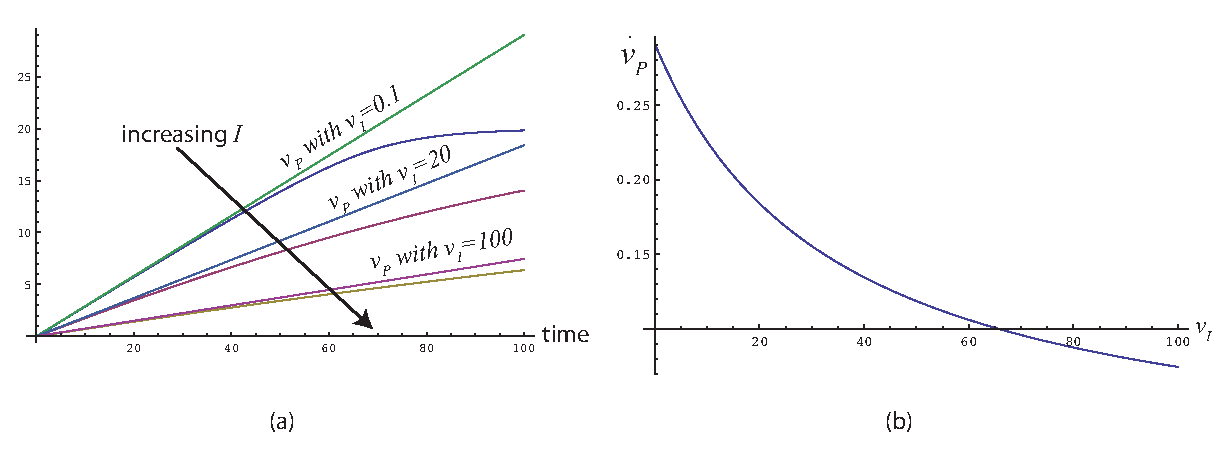
\epsfig{file=figures/comp-inhibit-together.eps, scale=0.65}
\caption{\label{fig:comp-inhibit} The competitive inhbition model. (a)
  Three different values for $v_I$ and the resulting dynamics for
  $v_P$ both the exact models (curves) and approximations (striaght
  lines). (b) As $v_I$ increases, the rate of production of $P$
  decreases.  }
\end{figure}


\section{Hill Functions}

Models of genetic regulatory networks can get big fast, in terms of
the number of species, the number of reactions, and the number of
unknown parameters. One way to reduce this complexity slightly is to
assume that regulatory interactions, such as the binding and unbinding
of a repressor to the regulatory region of a gene, are much faster than
the transcription and translation reactions. In fact, this is usually
a pretty safe assumption, although one has to be careful. The result
is to write rate of production of a gene's product in terms of the
{\em fraction} of action versus total gene:
%
\begin{equation} \label{eqn:gene-fraction}
\dot X = \alpha \frac{g_\mathrm{active}}{g_\mathrm{total}} + \alpha_0 - \beta X
\end{equation}
%
where $\alpha$ is the maximum rate of production, $\alpha_0$ is the
rate of ``leaky'' expression (sometimes used in these models, although
not strickly legitimate), and $\beta$ is the rate of protein
degradation and dilution. 

\begin{example}
Consider a gene $g$ repressed by a transcription factor $R$ via the following reaction
%
$$
g_\mathrm{on} + nR \xrightleftharpoons[\text{$k_{r}$}]{\text{$k_f$}} g_\mathrm{off} . 
$$
The number $n$, called the {\em cooperativity}, is the number of
molecules of $R$ that must bind to $g$ to turn it off. The reaction is
a bit unrealistic, as the likelihood that $n+1$ molecules
simultaneously interact and react is low for $n>1$. The idea is that
the reaction above is actually implemented by the sequential or
parallel binding of individual molecules $R$, one after the other. The
details of how different mechanisms affect the results in this example
are explored in the exercises (and see also \cite{hill-misuse}). 

\begin{figure}
\epsfig{file=figures/hill.eps, scale=0.8}
\caption{\label{fig:hill-repress} The Hill Function
  (Equation~\eref{eqn:hill-repress}) for repression plotted for
  various values of the cooperativity $n$. The function essentially
  computes the Boolean function $\neg R$. That is, when $R$ is not
  present, the gene is expressed. Otherwise it is not expressed.}
\end{figure}

If we assume that $k_r$ and $k_f$ are large, then, at equilibrium, we get
%%
$$
k_f g_\mathrm{on} R^n = k_r g_\mathrm{off} . 
$$
%%
Thus,
\begin{equation}\label{eq:hill-repress}
\frac{g_\mathrm{on}}{g_\mathrm{on}+g_\mathrm{off}} = 
  \frac{g_\mathrm{on}}{g_\mathrm{on}+\frac{k_f g_\mathrm{on} R^n}{k_r}} = \frac{1}{1+\frac{R^n}{K_\mathrm{eq}}} 
\end{equation}
where $K_\mathrm{eq} = k_r / k_b$ is the equilibrium constant of the
reaction. The result is a so called {\em Hill Function}
\cite{hill-function-1910} and is plotted in
Figure~\ref{fig:hill-repress} for various values of $n$. The Hill
function for repression inserted into
Equation~\eref{eqn:gene-fraction} results in 
%
$$
\dot X =  \frac{\alpha}{1+\frac{R^n}{K_\mathrm{eq}}}  + \alpha_0 - \beta X ,
$$
%
which describes the rate of production of a protein $X$ given the
concentration of the repressor $R$. This system essentially
  computes the Boolean function $\neg R$. That is, when $R$ is not
  present, the gene is expressed. Otherwise it is not expressed. \enx
\end{example}

\begin{example}
A similar function for activation can be obtained by considering the reactions
%
$$
g_\mathrm{off} + n A \xrightleftharpoons[\text{$k_{r}$}]{\text{$k_f$}} g_\mathrm{on} . 
$$
%
which results in the activation Hill Function
%
$$
\frac{g_\mathrm{on}}{g_\mathrm{on}+g_\mathrm{off}} = \frac{K_\mathrm{eq}A^n}{A^n + K_\mathrm{eq}},
$$
%
which can be substituted into Equation~\eref{eqn:gene-fraction} to
obtain a model for the production of a gene product as a function of
the activator concentration. 
%
\enx
\end{example}

\begin{figure}
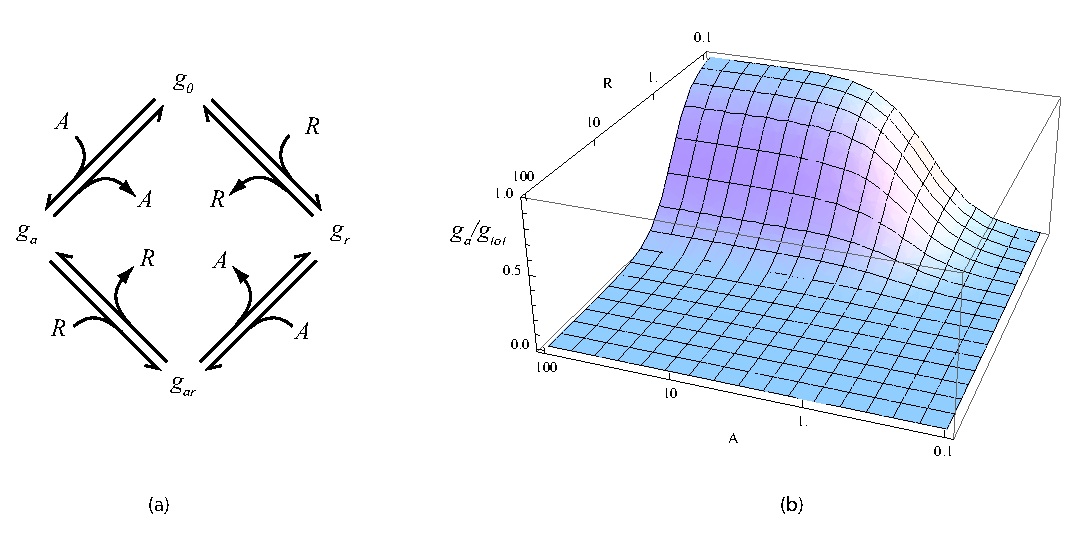
\epsfig{file=figures/act-rep.eps, scale=0.8}
\caption{\label{fig:act-rep} The Hill Function
  (Equation~\eref{eqn:alt-rep}) for a gene that is activated by a
  transcription factor $A$ and repressed by a transcription factor
  $R$.  The Hill function essentially computes the Boolean function $A
  \wedge \neg R$.  }
\end{figure}

\begin{example} (THERE ARE A BUNCH OF ERRORS IN THIS EXAMPLE TO BE
  FIXED) Many genes are regulated by several transcription factors,
  some that are activators, some that are inhibitors. Hill functions
  can be devised to model such situations as well. Here is an
  example. Suppose that a gene can be in one of four states: (1) $g_0$
  with no transcriptions factors bound; (2) $g_a$ with an activator
  bound; (3) $g_r$ with a repressor bound; (4) and $g_{ar}$ with both
  an activator and a repressor bound. The reaction network is shown in
  Figure~\ref{fig:act-rep}(a). At equilibrium, we have
%
\begin{eqnarray*}
k_1 g_0 & = & k_{-1} g_a \\
k_2 g_0 & = & k_{-2} g_r \\
k_3 g_a & = & k_{-3} g_{ar} \\
k_4 g_r & = & k_{-4} g_{ar} .
\end{eqnarray*}
Thus, the total amount of gene in the system is
%
\begin{eqnarray*}
g_\mathrm{tot} & = & g_0 + g_a + g_r + g_{ar} \\
 & = & g_0 + K_1 g_0 A^n + K_2 g_0 R^m + K_3 g_a R^m \\
 & = & g_0 + K_1 g_0 A^n + K_2 g_0 R^m + K_3  K_1 g_0 A^n R^m 
\end{eqnarray*}
where $K_i = k_i / k_{-i}$. From the above expression we obtain the Hill Function 
%
\begin{equation}\label{eq:alt-rep}
\frac{g_a}{g_\mathrm{tot}} = \frac{K_1 A^n}{1 + K_1A^n + K_2R^m + K_3  K_1A^n R^m}.
\end{equation}
%
This function is plotted for $m=n=2$ and $K_i=1$ in
Figure~\ref{fig:act-rep}(b). Only when the concentration of $A$ is
high and the concentration of $R$ is low is the gene active. In
logical terms, the system implements the Boolean function $A \wedge \neg R$. 
%
\enx
\end{example}

Warning: The cooperativity $n$ is a subject of some debate and
misuse. It is not unusual to find a paper stating that, for their
system, $n$ is not an integer! The reason is that Hill Functions are
used more to {\em fit} data than they are as first-principles models
like we are presenting them above. The student is warned to treat the
parameter $n$ with a grain of salt: It does not necessarily correspond
to anything physical. In fact, relieved of the need for a physical
meaning for $n$, we are free to treat it as just another parameter.




\section{Problems}

\setcounter{exercount}{0}

\begin{exercise}
Consider the system
%
$$
EA + S \xrightleftharpoons[\text{$k_{-1}$}]{\text{$k_1$}} EAS \xrightharpoon[\text{}]{\text{$k_2$}} EA + P
$$
$$
E + A \xrightleftharpoons[\text{$k_{-3}$}]{\text{$k_3$}} EA .
$$
%
in which an enzyme has an inactive form $E$ and an active form
$EA$. The molecule $A$ in this system is an activator. Determine an
enzyme kinetics model for this system similar to the competive
inhibition. That is, determine an approximate rate of product
production as a function of $v_S$ and $v_A$. Compare the mass action
kinetics model of the system with the appoximate version in simulation
to produce a plot similar to that in Figure~\ref{fig:comp-inhibit}(a).
\end{exercise}

\begin{exercise}
  Determine the Hill Function for the case of two activators where the
  active state of the gene is when both activators are bound to the gene.
\end{exercise}

\begin{exercise}
Consider the bistable switch described by
%
\begin{eqnarray*}
2A_1 & \rreact{k_1}{u_1} &  B_1  \\
2A_2 & \rreact{k_2}{u_2} &  B_2  \\
g_1 + B_2 & \rreact{\gamma_1}{\gamma_2} & g_{1,\mathit{off}} \\
g_2 + B_1 & \rreact{\gamma_1}{\gamma_2} & g_{2,\mathit{off}} \\
g_i & \react{\alpha} g_i + A_i \\
A_i & \react{\beta} & \varnothing
\end{eqnarray*}
%
Find equations for this system. Find two conservations and use them to
reduce the number of equations by two. Assume that the first four
reactions are fast and use the resulting equalities reduce the
equations further.
\end{exercise}

\chapter{Synthetic Regulatory Networks} 

\section{Re-programming {\em E. coli}}

% how we program it (plasmids, etc)

\subsection{Basic Genetic Engineering}

A nice feature of {\em E. coli}, and other organisms as well, is that
an {\em E. coli} cell may contain one or more pieces of small,
circular {\em plasmid} DNA. These independently replicating pieces of
DNA are processed inside the cell much the same way as is genomic
DNA. Furthermore, it turns out to be fairly easy to construct
synthetic plasmids and stick them inside appropriately prepared
cells. Once there, the ...

\subsection{How we See What's Going On}

how we see what is going on: fluorescence, micrsoscopy, gene arrays,
RT-pcr, flow-cytometry, etc. 

Regulation: Transcription factors, ribozymes and other mechanisms

Observables: GFP, FRET, populations, single cells

\subsection{Inducing and Tuning Behaviors}

Inputs: IPTG, UV, periodic inputs, etc.


\section{Switches and Oscillators}

As discussed in Chapter~\ref{ch:in_vivo}, we can hook up genes that
produce transcription factors to each other. Consider a set of genes
$g_1$, ..., $g_n$. Draw each gene as a circle. If a gene produces a
transcription factor that activates or represses another gene, we
write an arrow or a line with a bar respectively from one gene to the
other. If a small molecule, called an {\em inducer}, activates or
deactivates a transcription factor, we draw similar arrows from nodes
representing the molecule to the arrow representing an
interaction as shown in Figure~\ref{fig:grn}. 

Synthetic biologists have built such networks by borrowing
transcription factors and promotors the regulatory regions from
various organisms. We describe some of these efforts below.

\subsection{The Bistable Switch}

In 2000, researchers from James Collins' lab published one of the
first artificial genetic regulatory networks designed specifically to
demonstrate the computational or information processing potential of
genetic regulatory networks. The system was a bi-stable switch
\cite{collins-toggle} designed from a pair of repressors that each
repressed the expression of the other, as shown in
Figure~\ref{fig:toggle}. The transcription factors used in the paper
are the lactose inhibitor {\em lacI} from {\em E. coli} for the first
repressor, and either tetracycline resistance {\em tetR} or $\lambda$
from the bacteriophage $\lambda$ for the second. As discussed above,
{\em lacI} can be induced by IPTG. $tetR$ can be induced by
anhydrotetracycline, a derivative of tetracycline. Finally, $\lambda$
can be induced by heat. The inducers allow experimentors to switch the
toggle switch from one state to the other.

\begin{figure}
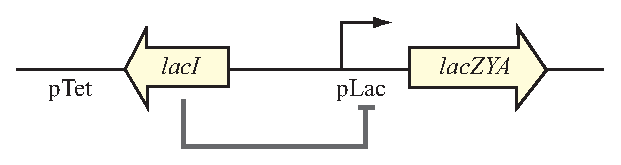
\epsfig{file=figures/toggle.eps, scale=0.8}
  \caption{\label{fig:toggle} The genetic toggle switch. Two
    repressors and their promotors are encoded on a plasmid. The first
    repressor is {\em lacI}, which acts on the pLac promoter. The pLac
    promoter is placed before the gene for the second repressor, which
    was either {\em tetR} or $\lambda$, and {\em gfp}. {\em tetR} acts
    on the pTet promoter, which is placed before {\em lacI}.}
\end{figure}

In the paper on the toggle switch, the authors propose the following
model
%
\begin{eqnarray}
X_1 & = & \frac{\alpha_1}{1+X_2^n} - X_1 \nonumber \\
X_2 & = & \frac{\alpha_2}{1+X_1^n} - X_2 . \label{eqn:bistable}
\end{eqnarray}
%
The authors note that bistability arises when the cooperativity
exceeds unity: $n,m>1$. For simplicity we assume that
$\alpha_1=\alpha_2=\alpha>0$.

\paragraph{The case when $n=m=1$:} When $n=1$, there is only on positive
equilibrium at
%
$$
X_1^* = X_2^* = \frac{-1 + \sqrt{1+4\alpha}}{2}.
$$
%
The Jacobian at this point is 
%
$$
A = \left . \left (
\begin{array}{cc}
-1 & -\frac{\alpha}{(1+X_2)^2} \\
-\frac{\alpha}{(1+X_2)^2} & -1 
\end{array}
\right ) \right |_{X=X^*}= 
\left (
\begin{array}{cc}
-1 & -\frac{4\alpha}{(1+X_2\sqrt{1+4\alpha})^2} \\
-\frac{4\alpha}{(1+X_2\sqrt{1+4\alpha})^2} & -1 
\end{array}
\right ) .
$$
%
The eigenvalues of $A$ are real and negative. Thus the single
equilibrium is stable and the system does not describe a bistable switch!

\paragraph{The case when $n=m>1$:} In this case, it is difficult to
obtain a closed form solution for $X^*$. One way to proceed is to
analyze the phase portrait. To do this, we define the following notion.

\begin{definition}
Given a two-dimensional system of the form 
\begin{eqnarray*}
\dot x_1 & = & f_1(x_1,x_2) \\
\dot x_2 & = & f_2(x_1,x_2),
\end{eqnarray*}
the first {\em nulcline} is the curve obtained by setting
$f_1(x_1,x_2) = 0$, i.e. where the first state variable $x_i$ is not
changing. The second {\em nulcline} is obtained via
$f_2(x_1,x_2)=0$. Anywhere two nuclines intersect is an equilibrium
point.
\end{definition}

The nulclines for the bistable swtich with $n=2$ and $\alpha=6$ are
shown, with the vector field defined by Equation~\ref{eqn:bistable},
in Figure~\ref{fig:bistable-nulclines}. Note that the nulclines
intersect in three points. Examination of various regions in the plot
indicates which are stable and which are not. For example, above the
two nulcines, all vectors point inward. Below, they point
outward. Along the nulcline for $\dot X_1 = 0$ and between the
separatrix (the blue line) and the top equilibrium point, $\dot X_2 >
0$. Along the $\dot X_2=0$ line and between the separatrix and the top
equilibrium point, $\dot X_1<0$. From this we can conclude that the
top equilibrium is stable. Similar reasoning shows the bottom
equilibrium is stable as well. 

\begin{figure}
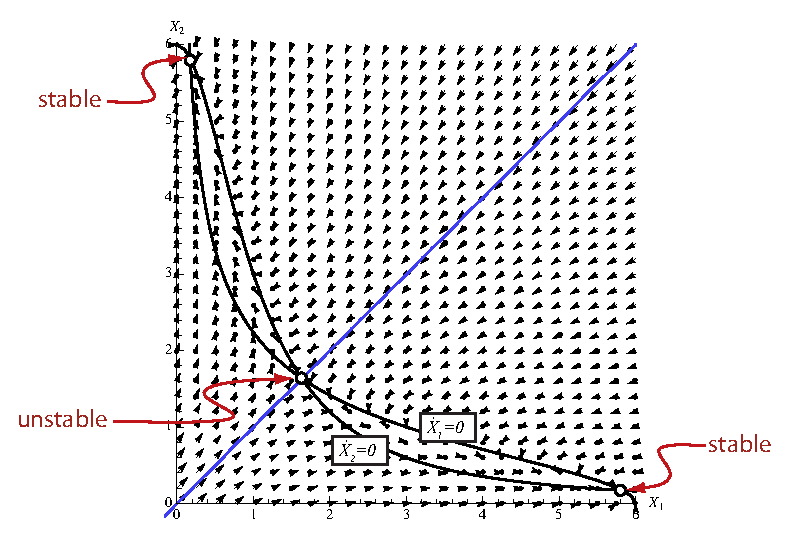
\epsfig{file=figures/bistable-nulclines.eps,scale=0.85}
\caption{\label{fig:bistable-nulclines} The nulclines and vector field
  associated with the bistable switch in Equation~\ref{eqn:bistable}
  with $n=2$ and $\alpha=6$. There are two stable equilibria and one
  unstable equilibrium.}
\end{figure}


\paragraph{No Cooperativity} There are papers stating that bistability
is in fact impossible with non-cooperative system
\cite{cherry-toggle}.  These papers use an extended Michaelis-Menton
somewhat blindly without recalling the assumptions that go into the
approximation. In particular, the assumption that there is a large
amount of $X_1$ cannot hold when there is a large amount of $X_2$. 

It turns out that a simple mass action model can produce bistability
without cooperativity. Consider the network
%
\begin{eqnarray*}
\varnothing \xrightharpoon[\text{}]{\text{$g_i \alpha_i$}} & X_i & 
            \xrightharpoon[\text{}]{\text{$\beta_i$}} \varnothing \\
g_1 + X_2 & \xrightleftharpoons[\text{$k_{-1}$}]{\text{$k_1$}} & g_{1,\mathit{off}} 
            \xrightharpoon[\text{}]{\text{$\gamma_1$}} g_1 \\
g_2 + X_1 & \xrightleftharpoons[\text{$k_{-2}$}]{\text{$k_2$}} & g_{2,\mathit{off}} 
            \xrightharpoon[\text{}]{\text{$\gamma_2$}} g_2 .
\end{eqnarray*}
%
Note that we have modeled the degradation of $X_i$ in two places. One,
$X_i$ simply degrades. Two, $X_i$ when bound to $g_j$ to make
$g_{j,\mathit{off}}$ degrades, turning $g_{j,\mathit{off}}$ into
$g_j$. We add this to the model, because when there is very little
$X_i$, the degradation of even the small amount of it that is bound to
$g_j$ is significant. 

It can be shown that the equation $\dot v = A K(v)$ has four
equilibria and that parameters can be found so that one has
$X_1=X_2<0$ while the other three have $X_1>0$ and $X_2>0$. The three
positive equilibra consist of two stable and one unstable equilibrium,
similar to the cooperative version of bistability above. 

\subsection{The Repressilator}

A construction similar to the bistable switch, and indeed appearing in
the same issue of Nature in 2000, is the ring oscillator made out of
three repressors \cite{elowitz-repressilator}, aptly named the
{\em repressilator}.

\subsection{Hysteresis Based Oscillators}

Circadian rhythms are responsible for many phenomena, the most famous
of which is the 17-year cycle of certain North American cicadas. Sleep
cycles in humans are another. The repressilator is not a likely model
for circadian rhythms, mostly because it is very sensitive to noise. A
more frequently proposed model for the kind of structure that likely
generates such oscillations is the {\em hysteresis based oscillator}
% http://www.nature.com/nature/journal/v403/n6767/pdf/403267b0.pdf
\cite{barkai-leibler-circadian}, which was to some extent implemented in 
% http://linkinghub.elsevier.com/retrieve/pii/S0092867403003465
\cite{ninfa-oscillator}.

% http://biodynamics.ucsd.edu/publications.htm
\cite{hasty-oscillator}

\subsection{A Bandbass Filter}

\cite{weiss-communication}

\section{RNA Regulatory Mechanisms}

Lock and key, ribozymes, etc.
\cite{rna-synthetic-biology}

\setcounter{exercount}{0}

\section{Problems}

\begin{exercise}
  Look up the equations used in the paper about the Repressilator
  \cite{elowitz-repressilator} and simulate them. 
\end{exercise}

\begin{exercise}
  Look up the equations used in the paper about the hysteresis-based
  oscillator that uses {\em araC} and {\em lacI}
  \cite{hasty-oscillator} and simulate them.
\end{exercise}

\chapter{{\em In vitro} Synthetic Biology}

In this chapter we explore biochemical networks that can be built {\em
  in vitro}, or in a test tube, out of simple molecules. We can use
short strands of DNA that interact in ways similar to how RNA
interacts inside cells, but without all of the other interactions seen
inside cells \cite{winfree-logic}. We can also add enzymes, such as
RNA polymerase, that allow us to explore transcription inside a test
tube \cite{kim-winfree-bistable}, once again without all of the other
interactions seen inside cells.

\section{Enzyme Free DNA Circuits}

\subsection{Mechanisms}

Hybridization, strand invasion, displacement, FRET.

\subsection{Design Constraints}

Sequence independence, toeholds and kinetics, secondary structure.

\subsection{Structure Prediction Software}

\subsection{The Design of an OR Gate}

\subsection{Three Different AND Gates}

In this section, we describe three different mechanisms for making an
AND gate. Each one uses the same reporter complex, which consists of
two strands as shown in Figure~\ref{fig:reporter}(a). The top strand
has the fluorophore, TAMRA, attached to it. The bottom strand has a
quencher, BHQ or Black Hole Quencher, attached to it. The reporter
does not fluoresce due to the proximity of the fluorophore and the
quencher. To use the reporter, an input strand can be introduced that
displaces the top strand. Once the top strand is displaced and moves
away from the quencher, the top strand fluoresces.

\begin{figure}
  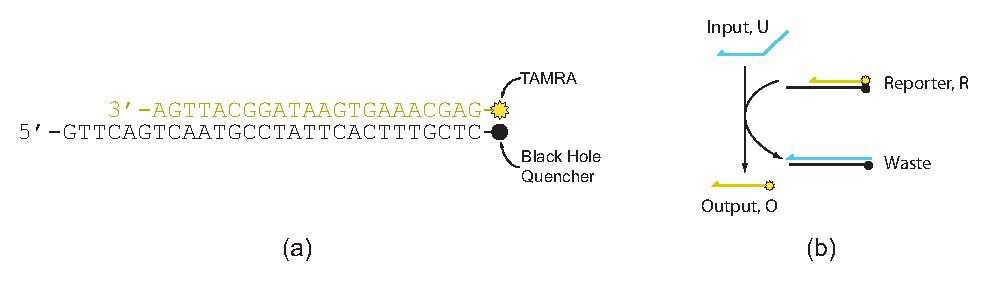
\epsfig{file=figures/invitro/reporter.eps, scale=0.8}
  \caption{\label{fig:reporter} The reporter used for the logic gate
    design problem. (a) Sequence design. (b) Use of an input strand to
    displace the fluorophore-labeled strand. }
\end{figure}

The first AND gate design, shown in Figure~\ref{fig:and1}, consists of a
backbone strand (grey) and a toehold strand (magenta) and an
intermediate strand (blue). The first input to the and gate, $A$,
attaches to the toehold and, through strand invasion, removes the
toehold strand, resulting in an intermediate complex and a waste
complex. Removing the magenta strand exposes a second toehold that is
complentary to part of input $B$, which attaches and displaces the
blue intermediate. The blue intermediate then interacts with the
reported to produce a fluorescent signal.

\begin{figure}
  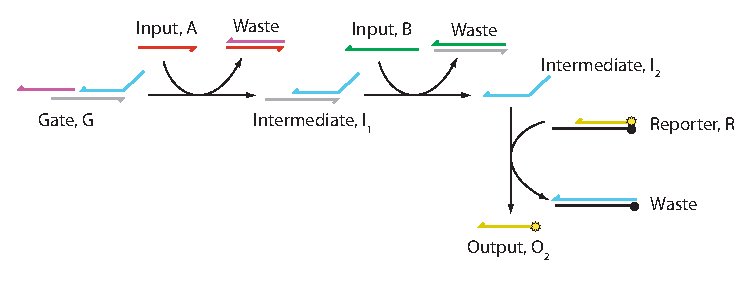
\epsfig{file=figures/invitro/and-1.eps}
  \caption{\label{fig:and1} First design for an AND gate. Input $A$ binds to the gate
    $G$, enabling input $B$ to bind.}
\end{figure}

The second AND gate design, shown in Figure~\ref{fig:and2}, is similar to the
first and gate, expect that the first input $A$ binds to the grey
backbone strand. The other main difference is that the input $A$ and
the magenta strand essentially compete as equals for the grey backbone
strand, making the first step of the process reversible. 

\begin{figure}
  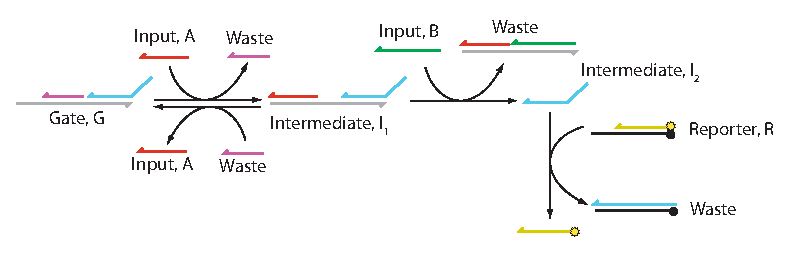
\epsfig{file=figures/invitro/and-2.eps}
  \caption{\label{fig:and2}Second design for an AND gate. Input $A$ binds to the gate
    $G$, enabling input $B$ to bind. This design differs from the
    first design in that $A$ can reversibly bind to the gate.}
\end{figure}

In both of the first two AND gate designs, input $A$ must bind to the
gate before $B$ can. The third AND gate design, shown in
Figure~\ref{fig:and3}, is symmetric in how the inputs attach to the
gate. Either can bind, and unbind first. Only once the second input
binds, the process cannot go back.

\begin{figure}
  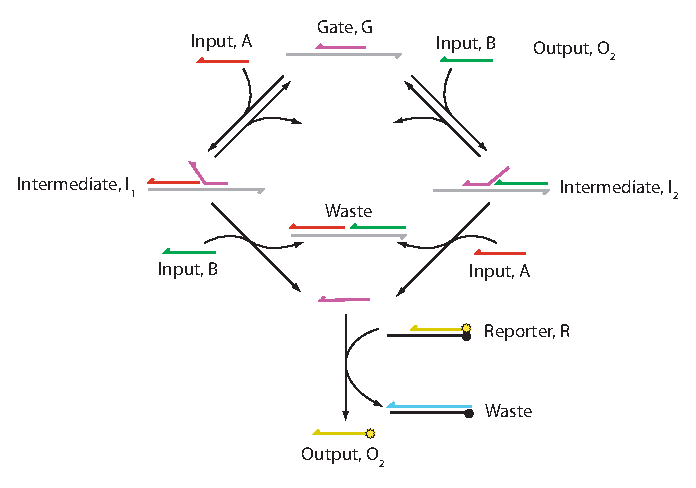
\epsfig{file=figures/invitro/and-3.eps}
  \caption{\label{fig:and3}Third design for an AND gate. Input $A$ and $B$ both
    reversibly binds to the gate $G$ to make an intermediate. The
    inputs can then bind irreversibly to complete the
    interaction. This allows the inputs to bind to the gate in either
    order.}
\end{figure}

\section{Transcriptional Circuits}

\section{Problems}

\setcounter{exercount}{0}

\begin{exercise}
  Describe each of the AND gates in
  Figure~\ref{fig:and1}-\ref{fig:and3} in terms of mass action
  kinetics and simulate them using mass action kinetics using all
  combinations of the presense or absense of the input strands. Assume the rate constants are identical
  for all bi-molecular reactions. 
\end{exercise}

\begin{exercise}
  In this problem you will design sequences to build your own DNA
  logic gate.  

  (a) Using the May 1, 2009 lecture as a guide, design sequences for
  an AND gate. Show the pairwise interactions between your strands
  predicted by NuPack, and also the results of each step in the
  reaction predicted by NuPack. You should name your sequences
  according to the scheme $GRPxSTDy$ where $x$ is your group number
  and $y$ is the strand number. Send your sequence designs to Kevin
  Oishi (koishi@u.washington.edu) by May 6 at 9:30 AM.

  (b) Simulate your AND gate using mass action kinetics using all
  combinations of the presense or absense of the input strands. Assume
  that the reaction rate for each step is proportional to the number
  of bases in the toehold region that initiate the interaction. Use
  the following table to determine which AND gate design to use:
\begin{center}
\begin{tabular}{l|l}
Group & Design \\
\hline
1 & 1 \\
2 & 2 \\
3 & 3 \\
4 & 1 \\
5 & 2 \\
6 & 3 \\
7 & 1 \\
8 & 2 \\
9 & 3 \\
10 & 1
\end{tabular}
\end{center}
\end{exercise}

\begin{exercise}
  Design a system of interacting DNA strands (using no enzymes
  whatsoever) that implements a three input AND gate. You can design
  the topology of the strands and the domains, but do not need to
  design the actual sequences (unless you want to). Show simulations
  of your system using reasonable assumptions for every combination of
  the three inputs.
\end{exercise}

\begin{exercise}
  (A Transcriptional Pulse Generator) (a) Design a transcriptional system
  (using DNA, RNA, RNAP and RNase H as in \cite{kim-winfree-bistable})
  that implements the following network: 
%
\begin{center}
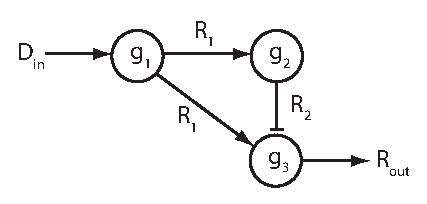
\epsfig{file=figures/trans-pulse.eps, scale=0.8}
\end{center}
%
where $g_1$, $g_2$ and $g_3$ are transcriptional swtiches, $R_1$,
$R_2$ and $R_\mathit{out}$ are RNA transcripts, and $D_\mathrm{in}$ is
a DNA input signal. For this we use a DNA input signal because we
don't want it to degrade via RNase H. Design the topology and the
domains, but not the sequences. (b) Derive equations for this system
based on regulatory network kinetics. (c) Simulate the system from an
initial condition in which all RNAs have zero concentration and
$D_\mathit{in}$ is a step input (i.e. it goes from zero to a nonzero
constant instantaneously). You should see a pulse in $R_\mathit{out}$.
\end{exercise}

\chapter{Stochastic Chemcal Kinetics} \label{ch:cme}

\section{Stochasticity in Cell Dynamics}

The formalism and example systems in the preceed chapters tacitly make
the assumption that there are so many molecules in the system of
interest that small fluctuations in the quantities, positions,
energies, etc. of these molecules do not contribute significantly to
the dynamics of the system. However, when we compare the behaviors of
individual isogenic cells, we see substantial variation in their
behaviors. For example, starting from isogenic and synchronized {\em
  E. coli} cells, the time between cell divisions is observed to be
highly variable, ranging from 30 to 60 minutes [CHECK THIS] at a given
temperature \cite{plank-harvey}. As another example, in bacterial
chemotaxis, cells respond to the addition of uniform attractant by
swimming smoothly, but relax back into tumbling at random times
\cite{spudich-koshland}. And as a third example, {\em E. coli} have
been see to switch to and from presenting type I {\em fimbriae} at
random time \cite{galley-fim}.

Two types of randomness have been proposed in the literature
\cite{swain-in-ex}: {\em Intrinsic} and {\em Extrinsic}. The former
has to do with randomness that is part of a system of interest and
that may be due to the fact that a given transcription factor may be
present in integral quantities: 0, 1, 2, etc. In this case, one has
to, for example, rethink what chemical equilibrium means: it may be
that on average the number of molecules of each type is fixed, but
reactions are still occuring and variations in the amounts of them can
be significant. The latter has to do with ...

% Examples from Elowitz, Van Oudenaarden, Arkin, etc.

\section{Foundations of Stochastic Chemical Reactions}

% assumptions
The common assumption in modeling stochastic chemical systems is that
the system is {\em well-mixed}. Mathematically, this means:
%
\begin{enumerate}
\item \label{wm1} The probability that a given pair of molecules
  reacts in the next $dt$ seconds is independent of time;
\item \label{wm2} A given molecule is equally likely to interact with
  every other molecule in the system.
\end{enumerate}
%
Physically, the assumptions \ref{wm1} and \ref{wm2} can arise if the
rate of diffusion is much higher than the rate of reaction, so that
the molecules are essentially uniformly distributed over the
containing volume. In this case, every instant of time is essentially
the same in terms of where the molecules are, and thus how the
molecules arrived there is irrelevant. 

Consider a vessel containing two molecules, $A$ and $B$, that react to
form a product molecule $C$ according to
%
$$
A+B \xrightharpoon[\text{}]{\text{$k$}} C
$$
%
where $k dt$ is defined to be {\em the probability that molecules $A$
  and $B$ react to form a $C$ in the time interval $[t,t+dt)$.}
Define by $f(t)$ the probability density function for when in time the
reaction occurs when the system is started at time $0$. Then
%
$$
F(t) = \int_0^t f(\tau) d \tau
$$
%
is the probability that the reaction occurs in time $[0,t]$. Suppose
the reaction has not occured by time $t$. Because the system is
well-mixed, we require that the probability density function $g(t)$
for when the reaction occur later, given that it has not occured at
time $t$, is distributed identically to $f(t)$, except shifted in
time. We can use this notion to determine an exact expression for
$f(t)$.

First, put
%
$$
G(t) = 1 - F(t)
$$
%
to be the cumulative distribution for the event that the reaction
occurs after time $t$.  Define $T$ be the random variable defining
when the reaction occurs, so that $G(t) = P[T>t]$. Then the well-mixed
assumption, essentially the same as the Markov assumption that future
events only depend on the current state of the process, requires that
%
$$
P[T>t+\tau | T > \tau] = P [T>\tau] .
$$
%
Using Bayes rule, we have
%
$$
P[T > t+\tau] = P[T>t] P[T>\tau], 
$$
%
which amounts to
%
$$
G(t+\tau) = G(t)G(\tau). 
$$
%
The only reasonable (integrable, analytic) function that satisfies the
above equation is the exponential, so that $G(t) = e^{-\alpha t}$ for
some $\alpha > 0$ (See Exercise~\ref{ex:exponential}). Since $F(t) = 1
- G(t)$ we have that
%
$$
F(t) = 1 - e^{-\alpha t}
$$
%
and $f(t) = \frac{d}{dt} F(t) = \alpha e^{-\alpha t}$. To determine
what $\alpha$ is, note that $F(dt) = k dt$ so that $f(0) = \left
  . \frac{d}{dt} F(dt) \right |_{t=0} = k$. Thus, $\alpha = k$ and
%
$$
f(t) = k e^{-k t} . 
$$
%
Therefore, the statistics of the reaction time are distributed
according to a Poisson waiting process with mean $1/k$. 

The $A$, $B$, $C$ system is a continuous time, discrete state Markov
process. The above derivation allows us to write it down as
such. First, note that the system has two states: state 1 in which the
reaction has not occurred and state 2 in which it has occured. The
rate at which we transition from state $1$ to $2$ is $k$. See
Figure~\ref{fig:two-state}. Typically, when talking about Markov
processes, we define the probability $p_i(t)$ of being in a particular
state $i$. We have already worked these probabilites out. We have
%
\begin{eqnarray*}
p_1 (t) & = & G(t) = e^{-k t} \\
p_2 (t) & = & F(t) = 1 - e^{-k t} .
\end{eqnarray*}
%
If we differentiate $p_1(t)$ we get $\dot p_1 = - k e{-kt} = - k
p_1$. Similarly, $\dot p_2 = k p_1$. We thus arrive a what is called
Kolmogorov's equation or the {\em Chemical Master Equation} for this
system:
%%
\begin{equation}
\dot p = Q p 
\end{equation}
%%
where $p$ is a vector of probabilities and, in this case, 
%
$$
Q = \left ( 
\begin{array}{cc}
-k & 0 \\
k & 0 
\end{array}
\right ) .
$$
%
The matrix $Q$ is called the infinitesimal generator or the {\em rate
  matrix} for the system.

\begin{figure}
\centering
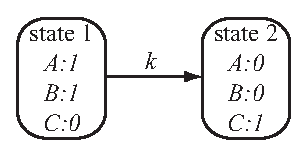
\epsfig{file=figures/two-state.eps, scale=0.7}
\caption{\label{fig:two-state} The Markov Process induced by the reaction 
$A+B \xrightharpoon[\text{}]{\text{$k$}} C$ .
}
\end{figure}




\section{Simple Examples}


In general, the rate matrix for a Markov process is constructed as
follows. The $Q_{i,i}$ matrix is the negative sum of the rates leaving
state $i$. The $Q{i,j}$ matrix, for $i \neq j$, is the rate from state
$j$ to state $i$. Furthermore, when $Q$ is small (say fewer than $1000
\times 1000$), the probability vector $p$ can be solved for explicitly:
%%
$$
p(t) = e^{Qt} p(0) .
$$
%%
All of the statistics, such as the mean copy number and variance of
particular species, can be obtained from $p(t)$.  Several examples are now
given.

\begin{example}
  Suppose we look at the same reaction, $A+B
  \xrightharpoon[\text{}]{\text{$k$}} C$, as above, except where there
  are initially $4$ $A$ molecules and $3$ $B$ molecules. This leads to
  a system with four states, which correspond to the number of $C$
  molecules in the system, either $0$, $1$, $2$, or $3$. Call
  these states $0$ though $3$. The rate at which the system progresses
  from state $0$ to state $1$ has to do with the probability that some
  $A$ reacts with some $B$ to produce a $C$. There are $4 \times 3 =
  12$ possible such pairs, and so probability of transition from state
  $0$ to $1$ in time $[0,dt)$ is $12k$. The rest of the transitions
  are similar. The entire Markov process is shown in
  Figure~\ref{fig:abc}.

\begin{figure}
\centering
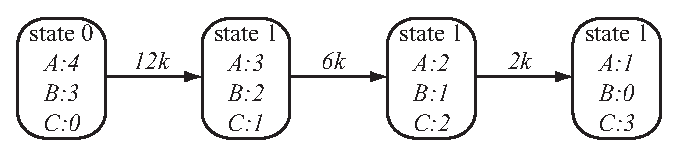
\epsfig{file=figures/abc.eps, scale=0.7}
\caption{\label{fig:abc} The Markov Process induced by the
  reaction $A+B \xrightharpoon[\text{}]{\text{$k$}} C$ where initially
  there are $4$ $A$s, $3$ $B$s, and $0$ $C$s.  }
\end{figure}

\begin{figure}
\centering
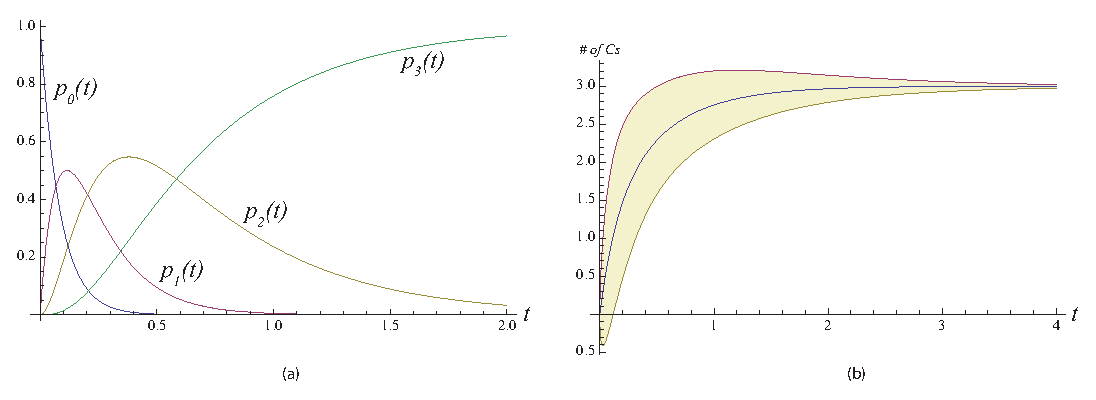
\epsfig{file=figures/abc-stats.eps, scale=0.7}
\caption{\label{fig:abc-stats} (a) The probabilities of being in one
  of the states of the Markov Process in Figure~\ref{fig:abc} versus
  time (for $k=1$). (b) The mean number of $C$s and the one-standard
  window. }
\end{figure}

Kolmogorov's equation for this system, $\dot p = Q p$, is
%
$$
\left ( \begin{array}{c}
\dot p_0 \\
\dot p_1 \\
\dot p_2 \\
\dot p_3 
\end{array}
\right ) = \left (
\begin{array}{cccc}
-12 k & 0 & 0 & 0 \\
12 k & 6k & 0 & 0 \\
0 & -6k & -2k & 0 \\
0 & 0 & 2 k & 0 
\end{array}
\right  )\left ( \begin{array}{c}
p_0 \\
p_1 \\
p_2 \\
p_3 
\end{array}
\right ) .
$$
%
This equation can be solved\footnotemark \ to obtain:
%
\begin{eqnarray*}
p_0(t) & = & e^{-12 t} \\
p_1(t) & = & 2 e^{-12 t} \left ( e^{6kt} - 1 \right ) \\
p_2(t) & = & 2\frac{3}{5} e^{-12 t} \left ( e^{2kt} - 1 \right)^2 \left ( 2 + 4 e^{2kt} + 6 e^{4kt} + 3 e^{6kt}\right ) \\
p_2(t) & = & 2\frac{1}{5} e^{-12 t} \left ( e^{2kt} - 1 \right)^3 \left ( 1 + 3 e^{2kt} + 6 e^{4kt} + 5 e^{6kt}\right )  .
\end{eqnarray*}
%
From the above expressions, we can obtain the mean number of $C$ molecules
%
$$
\ev C = \sum_i i p_i = 3 - \frac{1}{5} e^{-12 t} - e^{-6 t} - \frac{9}{5} e^{-2 t}
$$
%
and the second moment
$$
\ev{C^2} = \sum_i i^2 p_i = 9 - e^{-12 t} + e^{-6 t} - 9 e^{-2 t} .
$$
Figure~\ref{fig:abc-stats}(a) shows the probabilities versus time. The
initial state contains no $C$s. The probabilit of those states decays
exponentially. The probability of the intermediate states increases
and then decreases, and finally all the probability is absorbed in the
final state. Figure~\ref{fig:abc-stats}(b) shows the mean number of $C$s
and the one standard deviation window (calculated from $\ev{C}$ and
$\ev{C^2}$) for the reaction. 
\enx
\end{example}


\footnotetext{To find the solution to $\dot x = A x$ where $A$ is a
  matrix, we use the result that $x(t) = e^{At} x(0)$ where $e^A = I +
  A + A^2/2! + A^3/3! + ...$. The matrix $e^{At}$ can be found in
  MATLAB using the {\tt expm} function or in {\em Mathematica} using
  the {\tt MatrixExp} function.}


% A <-> B
\begin{example} \label{ex:ab}
Consider the reaction 
%
$$
A \xrightleftharpoons[k_2]{k_1} B
$$
and suppose we start with two $A$s and two $B$s for a total of $4$
molecules and five states. Then we arrive at a five state Markov
process with
%
$$
Q = \left ( \begin{array}{ccccc}
-4 k_2 & k_1 & 0 & 0 & 0 \\
4 k_2 & -k_1-3k_2 & 2 k_1 & 0 & 0 \\
0 & 3 k_2 & -2 k_1 -2 k_2 & 3 k_1 & 0 \\
0 & 0 & 2 k_2 & -3 k_1 - k_2 & 4 k_1 \\
0 & 0 & 0 & k_2 & -4 k_1
\end{array} \right ) 
$$
where index $i$ corresponds to the state in which there are $i$ $A$
molecules and $4-i$ $B$ molecules. 

If we start with some arbitrary number of molecules $n$, the
above matrix could only be written schematically, and it would be
difficult to obtain the moments of $A$ and $B$, as we did in the
previous example, in terms of $n$. In the next section, we describe a
method that sometimes workds for dealing with this kind of
problem. \enx
\end{example}

In general, if a system has a mass vector, so that new molecular mass
is not created, then resulting Markov process has a (possibly very
many) finite number of states. If a system can produce molecules from
nowhere, even if they are degraded at some rate, then there can in
principle be any number of such molecules in the system, resulting in
an infinite number of states. The next two examples describe
conservative and a non-conservative systems.

\begin{figure}
\centering
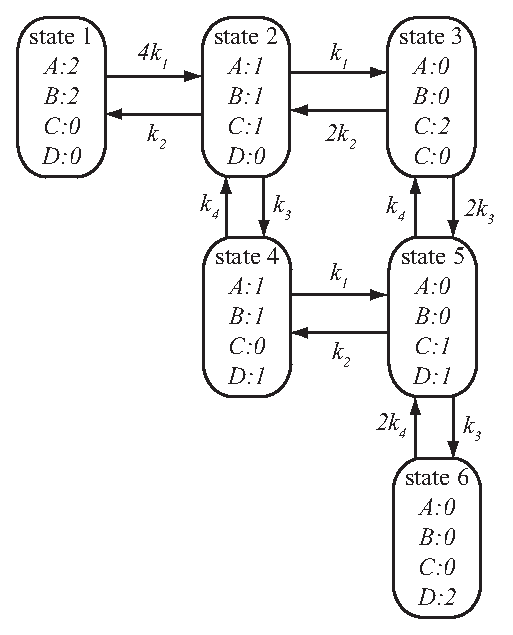
\epsfig{file=figures/cons.eps, scale=0.8}
\caption{\label{fig:cons} The Markov process for the chemical reaction in Example~\ref{ex:cons}.
}
\end{figure}

\begin{example} \label{ex:cons}
The system 
%
\begin{eqnarray*}
A + B & \rreact{k_1}{k_2}  & C  \\
C & \rreact{k_3}{k_4} D 
\end{eqnarray*}
is conservative (show this). The Markov process it produces, given
initially two $A$s, two $B$s and no $C$s or $D$s is shown in
Figure~\ref{fig:cons} and the resulting rate matrix is 
%%
$$
Q = \left (
\begin{array}{cccccc}
-4 k_1 & k_2 & 0 & 0 & 0 & 0 \\
4k_1 & -k_1-k_2 -k_3 & 2 k_2 & k_4 & 0 & 0 \\
0 & k_1 & -2k_2-2k_3 & 0 & 0 & 0 \\
0 & k_3 & 0 & -k_1 - k_4 & k_2 & 0 \\
0 & 0 & 2 k_3 & k_1 & -k_2-k_3 & 2 k_4 \\
0 & 0 & 0 & 0 & k_3 & -2k_4 
\end{array}
\right )
$$ \enx
\end{example}



% 0 -> X -> 0
\begin{example} \label{ex:stoch-gene-master} 
Consider the open-loop expression and degradation of a gene $X$ according to
%
$$
\varnothing \react{k_1} X \react{k_2} \varnothing .
$$
Probalistically speaking, this system can produce any number of $X$
molecules. The result is a Markov process with an infinite number of
states $0$, $1$, $2$, ... describing the number of $X$ molecules in
the system. We can describe the rate of change of the probabilities of
these states by the inifinite set of differential equations
%
$$
\begin{array}{rlllllll}
\dot p_0 & = & -k_1 p_0 & + k_2 p_1           &                  &                  &           \\
\dot p_1 & = &  \;\;\; k_1 p_0 & - (k_1+k_2) k_2 p_1 & + 2 k_2 p_2      &                  &           \\
\dot p_2 & = &          & \;\;\;k_1 p_1             & - (k_1+2k_2) p_2 & 3 k_2 p_3        &           \\
\dot p_3 & = &          &                     & \;\;\; k_1 p_2          & - (k_1+3k_2) p_3 & 4 k_2 p_3 \\
         & \vdots &     &                     &                  &                  & 
\end{array}
$$
Some useful information can be gained from this set of equations. For
example, the steady state distribution can be found as follows. First,
set the above equations to zero. The first equation gives
%
$$
p_1^* = \frac{k_1}{k_2} p_0^*.
$$
%
Adding the first two equations gives
%
$$
0 = -k_1 p_1^* + 2 k_2 p_2 *
$$
%
from which we obtain
%
$$
p_2^* = \frac{k_1}{2k_2}p_1^* = \frac{k_1^2}{2k_2^2} p_0^* .
$$
%
In general, adding the first $n$ equations gives
%%
$$
p_n^* = \frac{\alpha^n}{n!} p_0^*
$$
where $\alpha = k_1 / k_2$. Thus, we have all of the probabilities at
steady state in terms of $p_0^*$, which we can determine by noting
that the sum of the probabilities should be~1. That is
%
$$
\sum_{n=0}^\infty p_n^* = \sum_{n=0}^\infty \frac{\alpha^n}{n!} p_0^* 
                        = 1 \Leftrightarrow \sum_{n=0}^\infty \frac{\alpha^n}{n!} = \frac{1}{p_0^*} .
$$
%
The infinite sum evaluates to $e^{\alpha}$ so that $p_0^* = e^{-\alpha}$ and in general,
%
$$
p_n^* = \frac{\alpha^n}{n!}e^{-\alpha}.
$$
From this result, we can obtain, for example, the mean and second
moment:
%%
$$
\ev X^* = \sum n p_n^* = \alpha  = \frac{k_1}{k_2} 
$$
%%
and
$$
\ev{X^2}^* = \sum n^2 p_n^* = \alpha + \alpha^2 .
$$
%
Using the fact that the standard deviation of $X$ is $\sqrt{ \ev{X^2}
  - \ev X^2}$ be get that the simple result that the standard
deviation in $X$ is $\sqrt \alpha = \sqrt{k_1/k_2}$.
%
%%
\enx
\end{example}

\section{Moment Dynamics}

When there are an arbitrary number of molecules present in the system,
explicity enumerating the Markov process doesn't really work. For
example, consider Example~\ref{ex:ab} in which we enumerated the
states for $A \rreact{}{} B$ for two molecules. We might like to know
the statistics of how many molecules of $A$ we have at equilibrium,
independent of the initial number of $A$s and $B$s. The other problem
is that the system may have an infinite number of states, in which
case it may be difficult to reason about what is going on, although we
were successul with the example $\varnothing \react{} X \react{}
\varnothing$.

Another way to proceed is to use the {\em extended generator} to
produce the moment dynamics of a random variable of interest. Suppose
we have a reaction network with state space $S$ and having transitions
$1,2,3, ..., r$ with rates $k_1$, $k_2$, ..., $'k_r$. Define a {\em
  test function} over the state space by $\psi$. For example, $\psi$
might take a state $s$ and return the number of $A$ molecules in that
state.  The rate of change of the expected value of
$\psi$ follows the simple formula
%
\begin{equation} \label{eqn:moment}
\frac{d}{dt} \ev \psi = \ev{L \psi}
\end{equation}
%
where $L$ is the extended generator, defined by
%
\begin{equation} \label{eqn:generator}
L \psi = \sum_{i=1}^r ( \psi(s') - \psi(s) ) k_i .
\end{equation}
%
In the equation for $L$, we sum over all reactions $i$ the rate
$k_i$ times the difference of the value of $\psi$ after the reaction
and the valueof $\psi$ before the reaction. We can put any polynomial
we like into the equation for $\psi$, such as $A$ or $A^2$ to get the
rate of change of the first and second moments.

\begin{example}\label{ex:ab-moment}
Again, consider the reaction
%
$$
A \rreact{k_1}{k_2} B
$$
that we first encountered in example $\ref{ex:ab}$. This system has
two reactions, the rate of the first is $k_1 A$ and the rate of the
second is $k_2 B$. In general, the generator is
%
$$
L \psi = \left ( \psi \vvec{A-1}{B+1} - \psi \vvec{A}{B} \right ) k_1 A
       + \left ( \psi \vvec{A+1}{B+-1} - \psi \vvec{A}{B} \right ) k_2 B .
$$
%
We can use the generator to determine the rate of change of the
expected number of $A$ and $B$ molecules. We have
%
\begin{eqnarray*}
L A & = & ( A - 1 - A ) k_1 A + ( A + 1 - A ) k_2 B = -k_1 A + k_2 B \\
L B & = & ( B + 1 - B ) k_1 A + ( B - 1 - B ) k_2 B = k_1 A - k_2 B
\end{eqnarray*}
%
Therefore, using Equation~\eref{eqn:moment} we have
%
\begin{eqnarray*}
\frac{d}{dt} \ev A & = &  - k_1 \ev A + k_2 \ev B \\
\frac{d}{dt} \ev B & = &  k_1 \ev A - k_2 \ev B .
\end{eqnarray*}
%
We can also determine the second moment dynamics. These are given by
%
\begin{eqnarray*}
L A^2 & = & ( ( A-1 )^2 - A^2 ) k_1 A + ( ( A+1 )^2 - A^2 ) k_2 B \\
      & = & ( -2A + 1 ) k_1 A + ( 2A + 1 ) k_2 B \\
      & = & k_1 A - 2 k_1 A^2 + k_2 B + 2 k_2 A B .
\end{eqnarray*}
Notice that if we put the above into the Equation~\eref{eqn:moment},
we would get the rate of change of $\ev{A^2}$ in terms of the moments
$\ev A$, $\ev B$, and $\ev{A^2}$ (which we already know), but also
$\ev{AB}$. We could expand this as well, but note that $A+B=n$ is
constant. So instead, we get
%
\begin{eqnarray*}
\frac{d}{dt} \ev{A^2} & = & k_1 \ev A - 2 k_1 \ev{A^2} + k_2 n - k_2 \ev{A}
        + 2 k_2 n \ev A - 2 k_2 \ev{A^2} \\
 & = & k_2 n + ( k_1 - k_2 + 2 k_2 n ) \ev A - 2 ( k_2+k_1 ) \ev{A^2} . 
\end{eqnarray*}
Note: we could also have eliminated the equation for $\ev B$ and the
result would be the rates of change of $\ev A$ and $\ev{A^2}$ in terms
of $\ev A$ and $\ev{A^2}$ .
%
\enx
\end{example}

\begin{example}\label{ex:gene-moment}
Consider again the gene expression example
%
$$
\varnothing \react{k_1} X \react{k_2} \varnothing .
$$
%
We have for the first moment
%
$$
L X = k_1 - k_2 X
$$
%
so that 
%
$$
\ev X = k_1 - k_2 \ev X
$$
%
and $\ev X^* = \frac{k_1}{k_2}$. For the second moment
%
\begin{eqnarray*}
L X^2 & = & ( (X+1)^2 - X^2 ) k_1 + ( (X-1)^2 - X^2 ) k_2 X \\
      & = & ( 2X + 1 ) k_1 + ( -2X+1 ) k_2 X \\
      & = & k_1 + ( 2k_1+k_2 ) X -2 k_2 X^2
\end{eqnarray*}
so that
%
$$
\ev{X^2} = k_1 + (k_1+k_2) \ev X - k_2 \ev{X^2} .
$$
%
At equilibrium, we have
%
\begin{eqnarray*}
\ev{X^2} & = & \frac{k_1 + (2k_1+k_2)\frac{k_1}{k_2}}{2k_2} \\
         & = & \frac{k_1}{k_2} + \frac{k_1^2}{k_2^2}
\end{eqnarray*}
which is the same result as in Example~\ref{ex:stoch-gene-master}. 
%
\enx
\end{example}

The extended generator is a powerful tool for accessing the statistics
of a stochastic chemical reaction, but it does have limitations, which
we now describe. Suppose a system has molecules $A$, $B$, $C$. The
moments of interest are usually the first moments $\ev A$, $\ev B$,
$\ev C$ and the second moments $\ev{A^2}$, $\ev{AB}$, $\ev{AC}$,
$\ev{B^2}$, $\ev{BC}$, etc. There are higher order moments too, such
as $\ev{A^2BC^3}$, but one typically is not concerned with these. One
promising looking result is that the dynamics of each moment are
linear in the rest of the moments. That is, if we stack all the
moments in an infinite dimensional vector $\mu$, then $\dot \mu = A
\mu + B$ describes the rate of change of all the moments, where $A$ is
an infinite dimensional matrix and $B$ is an infinite dimensional
vector.

However, it may be that lower order moments depend on high order
ones. This is not the case in Examples~\ref{ex:ab-moment}
and~\ref{ex:gene-moment} where the rate of change of the first moments
depend on only the first moments; the rate of change of the second
moments depend on the rate of change of the first and second; and so
on. We call this property {\em moment closure}: The rates of change of
all moments depend only on themselves and lower order moments. This
property, when present, makes the moment equations easy to solve.  A
general result, that the above two examples share, is as follows.

\begin{theorem}
  The moment dynamics of a system of reactions in which each reaction
  is no more than unimolecular (involving one or fewer reactants) are closed.
\end{theorem}

For bimolecular reactions, which includes many systems of interest,
the moments are typically not closed, as the following example shows.

\begin{example}
Considera again the reaction
%
$$
A + B \react{k} C .
$$
%
Note that if there are initially $n_A$ As, $n_B$ Bs and zero $C$s, we
have the conservation laws $A = n_A - C$ and $B = n_B - C$. Therefore,
we can simply look at the moments of $C$. We have
%
$$
L C^n = \left ( (C+1)^n - C^n \right ) A B k = \left ( (C+1)^n - C^n \right ) ( n_A - C ) ( n_B - C ) k, 
$$
%
which is an $n+1$ order polynomial. Thus $\ev{C^n}$ depends on
$\ev{C^{n+1}}$ and the moments are not closed.
%
\enx
\end{example}


\section{Approximate Methods}

% approximating the state space

A discussion of the finite state projection algorithm goes here.

\section{Simulation}

Analytical methods for solving stochasti processes are hard to come
by, and are not always easy to analyze. A common recourse is to 

Simulating stochastic processes can be difficult. A naive approach,
and one that is really the best you can do for arbitrary stochasti
processes, is to choose what will happen in the next $delta$ seconds,
where $\delta>0$ is a small number. For example, if there are two
reactions that can occur, one with rate $k_1$ and one with rate $k_2$,
then one would roll a three sided die with weights
%
$$
p_1 = \delta k_1, \;\; p_2 = \delta k_2, \;\; p_3 = 1 - \delta(k_1+k_2) . 
$$
%
If the die comes up with option 1 or 2, the state is updated. If the
die comes up with option three, the state is not update. Then the time
is updated by $\delta$ seconds and the process continues. 

There are several problems with this approach. First, it is
approximate: The trajectories obtained in this manner are not exactly
drawn from the correct distribution, although they sampling becomes
more correct as $\delta \rightarrow 0$. Second, if $\delta$ is small,
then the only thing that happens in most steps is that the time is
updated. This is because the probability that something happens in the
next $\delta$ seconds approaches zero as $\delta$ approaches zero! So
the more accurate the simulation, the longer it takes to simulate.

% the hard way: k dt

Continuous time Markov processes are actually much easier to
simulate. The observation that one can ``exactly'' simulate the Markov
process arising from a stochastic chemical reaction is due to
Gillespie \cite{gillespie}. The algorithm is called the {\em
  Stochastic Simulation Algorithm} or SSA, but is oftern referred to
as the {\em Gillespie Algorithm}.

To explain how it works, consider a Markov process with states
$1,2,3,...$. Suppose the current state is $i$ at time $0$. We would
like to know the joint probability $P[t,j]$ that the next transition
is from $i$ to $j$ and occurs in time $[t,t+dt]$. We can use the rate
$k_{i,j}$, which is the probability that an $i$ to $j$ transition
occurs in the next $dt$ seconds, to get
%
\begin{equation} \label{eqn:Ptj}
P[t,j] = P[T>t] k_{i,j} dt
\end{equation}
%
where $P[T>t]$ is the probability that the transition does not occur
in time $[0,t]$.

We can derive a similar expression for $P[T>t+dt]$. First note that 
%
$$
\left ( 1 - \sum_{j=1^N} k_{i,j} \right ) dt = ( 1 - K_i )
$$
%
is equivalent to the probability that no transition occurs in the next
$dt$ seconds. Here, we have defined $K_i = \sum_{j=1}^N k_{i,j}$ to be
the total rate out of state $i$. Thus,
%
$$
P[T>t+dt] = P[T>t] ( 1 - K_i ) dt . 
$$
Rearranging gives
%
$$
\frac{P[T>t+dt] - P[T>t]}{dt} = - P[T>t] K_i.
$$
%
The left hand side of this is $\frac{d}{dt}P[T>t]$. Solving this
differential equation for $P[T>t]$ and substituting into
Equation~\eref{eqn:Ptj} gives
%
\begin{equation}\label{eqn:ssa-pdf}
P[t,j] = k_{i,j} e^{-K_i t} .
\end{equation}
%
We can now determine how to choose the next state and the next reaction time.

\paragraph{Next Reaction:} Integrating Equation~\eref{eqn:ssa-pdf}
over all time gives the probability that the next reaction is $j$, no
matter what time it occurs.
%
\begin{equation}\label{eqn:next-reaction}
p_{i,j} = \int_0^\infty  k_{i,j} e^{-K_i t} dt = \frac{k_{i,j}}{K_i} .
\end{equation}
%
Thus, to choose the next reaction, we roll an $N$ sided die, with
weights $p_{i,j}$ for $j=1,N$.

\paragraph{Reaction Time:} To choose the time, we sum over all
reactions to get that the proabilility densitiy function for the next
reaction time is
%
$$
\sum_{j=1}^N k_{i,j} e^{-K_i t} = K_i e^{-K_i t}. 
$$
%
The cumulative distribution function corresponding to this function is
%
$$
\int_0^t K_i e^{-K_i t\tau} d \tau = 1 - e^{-K_i t} = r \in [0,1],
$$
which relates $t$ distributed according to the Poisson distribution
$K_i e^{-K_i t}$ and $r$ distributed uniformly in $[0,1]$. Since
computers can pick uniform random numbers easily, we solve for $t$ to
get
%
\begin{equation}\label{eqn:next-time}
t = \frac{1}{K_i} \ln \frac{1}{1-r} .
\end{equation}
%
Therefore, to choose the next time in a simulation, we choose $r$
uniformly in $[0,1]$ and then compute the time according to the above.

\paragraph{The SSA:} Now, using the above results, we describe the
Stochastic Simulation Algorithm. 
\begin{enumerate}
\item[1.] Choose an initial condition $v$ equal to some vector of the copy
  numbers of the species in the reaction network.
\item[2.] Set $t=0$.
\item[3.] For each reaction $\rho$ applicable in $v$, determine the rate $k_v$. 
\item[4.] Choose the next reaction via Equation~\ref{eqn:next-reaction}.
\item[5.] Choose the $\Delta t$ via Equation~\ref{eqn:next-time} and set
  $t$ to $t+\Delta t$. 
\item[6.] Goto 3.
\end{enumerate}

In practice, one typically sets a maximum time and a maximum number of
steps to force a termination condition. Also, a single trajectory is
usually not sufficient to characterize the behavior, so multiple
trajectories are sampled (say thousands) and combined to obtain sample
averages. 

\begin{figure}
  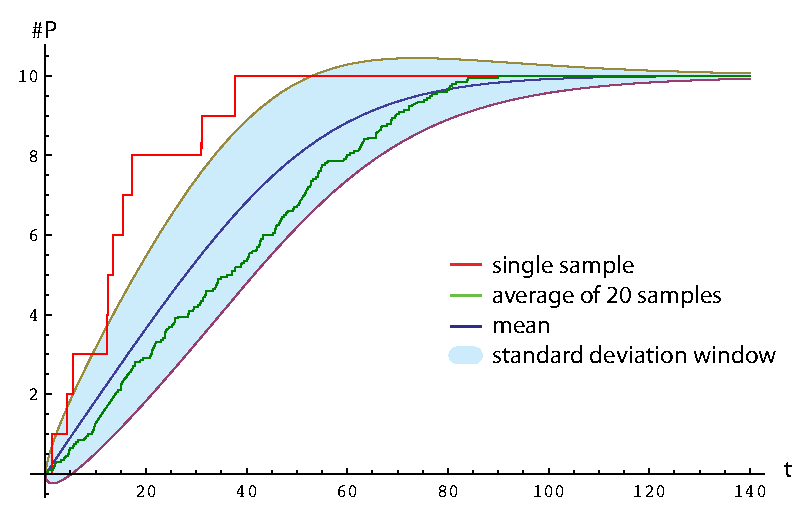
\epsfig{file=figures/stochastic-mich-ment.eps, scale=0.7}
  \caption{\label{fig:mm-stoch} The Michaelis-Menton system from
    Example~\ref{ex:mm-stoch}. Shown are a sample trajectory (red), 20
    samples averaged together (blue) and the mean and standard
    deviation window computed from the Kolmogorov Equation. }
\end{figure}

\begin{example} \label{ex:mm-stoch}
Consider the reaction network
%
$$
E + S \rreact{k_1}{k_2} ES \react{k_3} E + P 
$$
where $k_1=1$, $k_2=0.5$ and $k_3=0.1$. Starting in a state $v_1 =
(E,S,ES,P) = (2,10,0,0)$ at time $t=0$, the only reaction applicable
is the first. Thus the probability that the next state is $(1,9,1,0)$
is $1$. The reaction has rate $20 k_1 = 20$. The time the reaction
occurs is distributed according to the p.d.f. $20 e^{-20t}$. From the
state $(1,9,1,0)$ there are three possible reactions with rates
%
$$
9, \; 0.5, \; \mathrm{and} \; 0.9 .
$$
Thus, the probabilities of each of these reactions are
%%
$$
\frac{9}{10.4}, \; \frac{0.5}{10.4}, \; \mathrm{and} \; \frac{0.9}{10.4}
$$
%
and the p.d.f. of when the reaction occurs is distributed according to
$10.4 e^{-10.4 t}$. Figure~\ref{fig:mm-stoch} shows a typical sample
trajectory along with the average of 20 samples, and the mean and
variance computed from the Kolmogorov Equation in which all 30 states
are enumerated. 
%
\end{example}



\section{Computing with Molecules}

One of the central questions of synthetic biology is whether and how
computations can be carried out with molecular systems. Many
researchers have tried to answer this question and computations have
been done with oligos \cite{adleman-science94} and DNA self-assembly
\cite{winfree-assembly} for example. Furthermore, many models of
molecular computation have been proposed
\cite{rozenberg-dna-computing}. Here, we examn one such model, which
is an implementation of regiester machines \cite{minsky-rms} by
stochastic chemical reaction networks \cite{soloviechik-rm}.

A {\em register machine} is a kind of abstract computational
machine. It is equivalent in expressibility to the Turning Machine
model, and thus any algorithm can in principle be implemented as a
register machine. Register machines consist a finite set of states
$S_0$, $S_1$, ..., $S_n$ and a set of registers $R_0$, $R_1$, ...,
$R_m$. Register machine transitions have of two types. The first is an
increment:
%
$$
\mathrm{inc}(i,r,j)
$$
%
which means {\em if the state is $i$, then increase register $r$ and
  go to state $j$}. The second is a decrement:
%
$$
\mathrm{dec}(i,r,j,k)
$$
%
which means {\em if the state is $i$ and register $r$ is greater than
  zero, then decrease register $r$ and go to state $j$; otherwise go
  to state $k$.}. 

Register machines can be written as diagrams, as in
Figure~\ref{fig:rm-mult}, which describes a register machine that can
multiply. The increment transitions are simply arrows from $i$ to $j$
with the register $r$ being incremented shown by the arrow. For
example, the arrow from state $2$ to $3$ labeled $\uparrow 2$
describes the command $\mathrm{inc}(2,2,3)$. The decrement transitions
are similar, except that a dashed arrow describes what state to go to
if the register being decremented is zero.

\begin{figure}
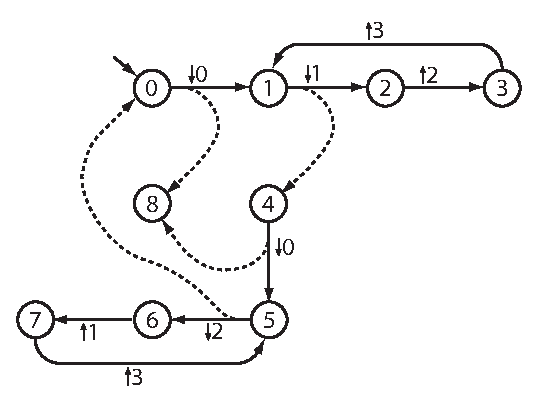
\epsfig{file=figures/rm-mult.eps, scale=0.9}
\caption{\label{fig:rm-mult} A register machine that multiplies the
  initial contents of registers $0$ and $1$. Register $3$ holds the
  final value and register $2$ is swap space.}
\end{figure}

To implement a register machine with stochastic chemical reactions, we
do the following. First, introduce a new chemical species $S_i$ for
each sate. We will require that at any given time, the total number of
state molecules of any kind is $1$. Also, we introduce new chemical
species $R_i$ for every register. The number of $R_i$ molecules in the
system at a given time corresponds to the value of that register at
that time. Next, for each increment transition $\mathrm{inc}(i,r,j)$
in the system we introduce the reaction
%
$$
S_i \react{k} S_j + M_r. 
$$
%
Finally, for each decrement transition $\mathrm{dec}(i,r,j,k)$ we
introduce the two reactions
%
$$
S_i + M_r \react{k} S_j
$$
and
$$
S_i \react{\varepsilon} S_k .
$$
%
The first decrement reaction describes the interaction of an $S_i$
molecule with an $M_r$ molecule. This reaction has rate $M_r k$ so
that if there are no $M_r$ molecules, the reaction rate is zero. The
second reaction is the ``else'' part of the decrement rule. If there
are no $M_r$ molecules, then eventually this section reaction should
occur. However, there is some small probability
%
$$
\frac{\varepsilon}{\varepsilon+M_r k}
$$
%
that the second decrement reaction might occur even if there are $M_r$
molecules around. Thus, we would like $\epsilon$ to be small. On the
other hand, when it is not an error to take the second decrement
reaction, we sould like the rate to be large. This tradeoff is
fundamental to this formulation: {\em accurate computation takes
  longer}.

\begin{figure}
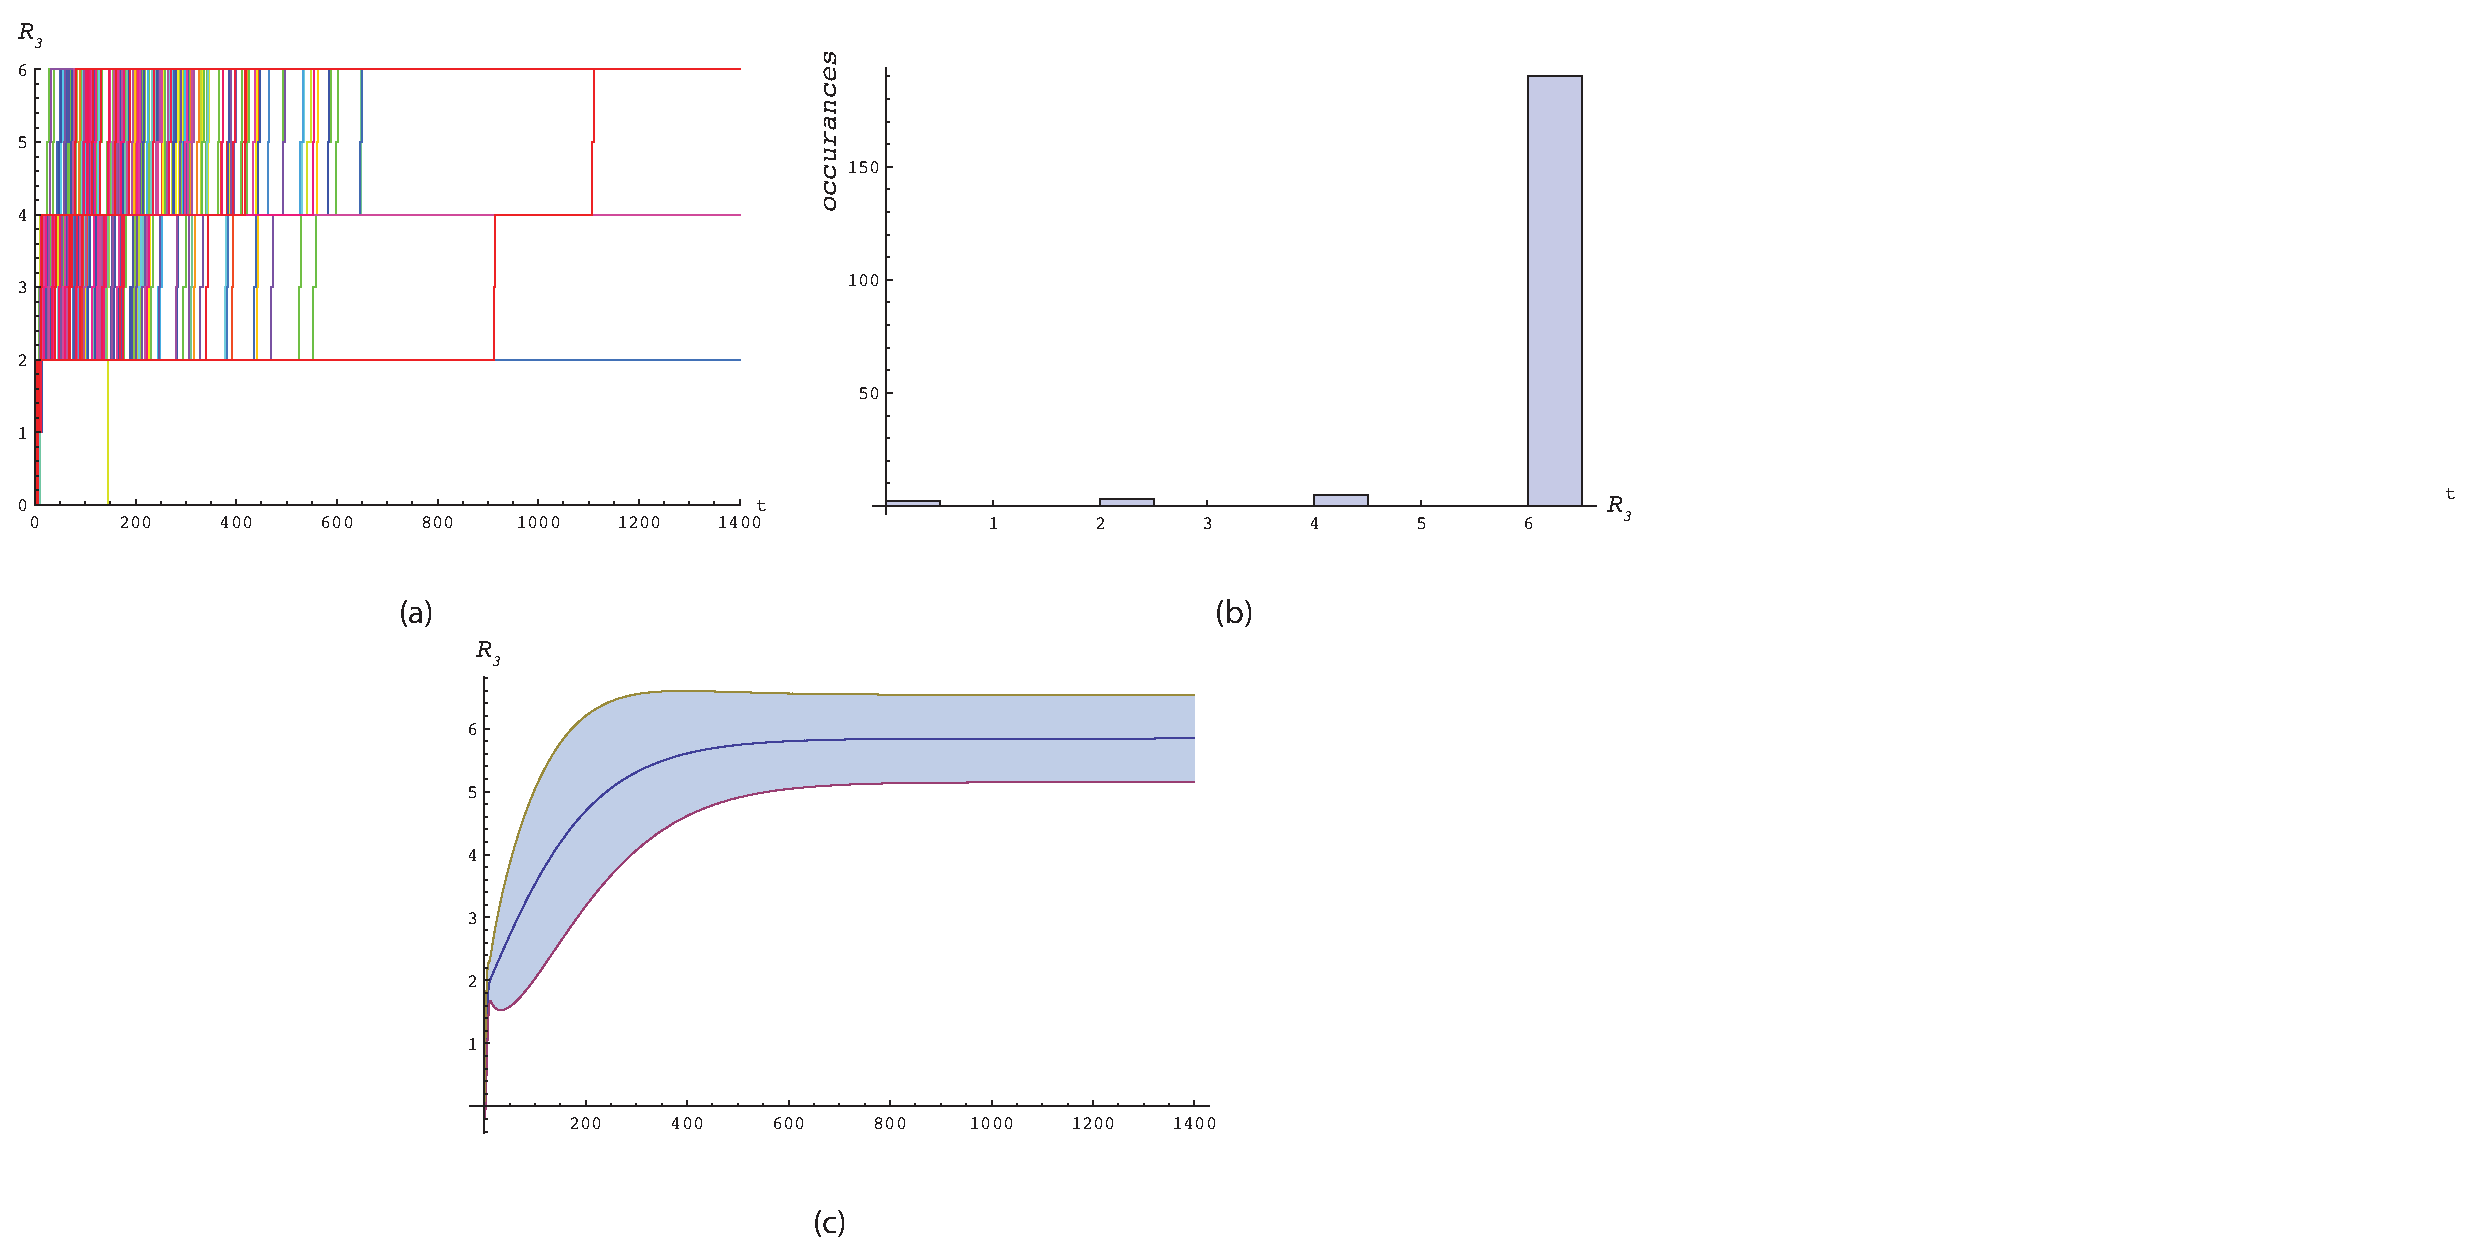
\epsfig{file=figures/rm-behavior.eps, scale=0.45}
\caption{\label{fig:rm-mult-data} (a) Several trajectories of the
  chemical implementation of the multiplication register machine
  computing $2 \times 3$. (b) The histogram of the computed
  results. (c) The mean and standard deviation behavior computed from
  the Kolmogorov equation.}
\end{figure}


\begin{example}
  The register machine\footnotemark in Figure~\ref{fig:rm-mult}
  multiplies the contents of registers $R_0$ and $R_1$ and puts the
  result in register $R_3$. This can be implemented with twelve
  reactions: two each for the decrement reactions and one each for the
  increment reactions. Figures~\ref{fig:rm-mult-data}(a) and~(b) shows
  the resulting behavior when computing $2 \times 3 = 6$ with $k=1$
  and $\epsilon=0.01$. Stochastic simulations show the system can end
  up with the result $0$, $2$, $4$ and $6$ with the most likely answer
  being the correct one. Figure~\ref{fig:rm-mult-data}(c) shows the
  exact solution. Using the methods in this chapter, the entire state
  space (of the Markov process) was enumerated to yield 78 states and
  a $78 \times 78$ dimensional rate matrix. Shown are the average
  number of $R_3$ molecules and the standard deviation window. \enx
\end{example}

\footnotetext{The author thanks Kevin Oishi for finding a way to
  multiply with register machines.}




\section{Problems}

\setcounter{exercount}{0} 

\begin{exercise}\label{ex:exponential}
  Show that if $G(t+\tau) = G(t)G(\tau)$ is analytical and integrable,
  then $G(t) = e^{-\alpha t}$ for some $\alpha > 0$.
\end{exercise}

\begin{exercise}
Consider the reaction network
%
\begin{eqnarray*}
A & \react{k_1} & B + C \\
C + D & \rreact{k_2}{k_3} & E 
\end{eqnarray*}
%
starting with two $A$s and two $D$s and no $B$s, $C$s or $E$s. (a)
Enumerate the states and draw the Markov process the results from this
system. (b) Determine the rate matrix. (c) Find the probabilities of
being in each state as a function of time by finding $e^{Qt}p(0)$. (d)
Find the mean and variance for the number of $E$s as a function of
time and plot the mean and the one standard deviation window versus
time (as in Figure~\ref{fig:abc-stats}(c)) assuming all the rates are
unity. Note: To simiplfy things, you may set $k_1=1$, $k_2=1$, and
$k_3=1$. Also, if you use MATLAB or Mathematica to compute the
solution, you do not need to show the output if it is large, just show
the code.
\end{exercise}

\begin{exercise}
  Show that if a system of reactions admits a mass vector, then the
  Markov process describing its stocahstic behavior has a finite
  number of states. Give an example of a non-conservative system that
  still produces a finite number of states.
\end{exercise}

\begin{exercise}
  For the gene production and degradation system described in
  Examples~\ref{ex:stoch-gene-master} and~\ref{ex:stoch-gene-moments},
  determine the number $n$ such that the probability of there being
  more than $n$ molecules of $X$ at steady state is less than 1\%. 
\end{exercise}

\begin{exercise} \label{exer:ab-probs}
  Determine the time varying probabilities of being in the various
  states of Example~\ref{ex:ab}. Plot the probabilities versus time
  for the case when both rates are~1 and we start with no $B$
  molecules.
\end{exercise}

\begin{exercise}
  Verify that the moment equations for $\ev A$ and $\ev{A^2}$ obtained
  in Example~\ref{ex:ab-moment} match those obtained using the
  solutions from Exercise~\ref{exer:ab-probs}. 
\end{exercise}



\begin{exercise}
Consider the system
%
$$
\varnothing \react{k_1} X \react{k_2} Y \react{k_3} \varnothing .
$$
Using equations~\eref{eqn:moment} and~\ref{eqn:generator}, determine
equations for $\ev X$, $\ev Y$, $\ev{X^2}$, and $\ev{Y^2}$ versus
time. Determine the steady state values for the means and standard
deviations. Starting from no molecules, plot the expected number of
$X$ and $Y$ molecules and standard deviation windows (as in
Figure~\ref{fig:abc-stats}(c)) assuming the rates are all unity.
%
\end{exercise}



\begin{exercise}
\item Consider the network
%
$$
EA+S \rreact{k_1}{k_{-1}} EAS \react{k_2} EA + P
$$
$$
E+A \rreact{k_3}{k_{-3}} EA
$$
\noindent
with rates

\hspace{0.5in}\begin{tabular}{ll}
$k_1$    & 9.3 $s^{-1}$ \\
$k_{-1}$ & 1.2 $s^{-1}$ \\
$k_2$    & 0.5 $s^{-1}$ \\
$k_3$    & 5.0 $s^{-1}$ \\
$k_{-3}$ & 1.5 $s^{-1}$. 
\end{tabular}
\begin{enumerate}
\item[a)] Suppose the initial number of $E$, $A$ and $S$ molecules is 2, 1
  and 4 respectively and the initial number of the remaining molecule
  types is 0. Draw the Markov process that results.
\item[b)] Plot the mean and standard deviation window for the number
  of $P$ molecules as a function of time, as in
  Figure~\ref{fig:mm-stoch}. You should obtain these either by solving
  the Kolmogorov Equation via $e^{Qt}$ or simply simulating the
  differential equations. You should find $\ev P$ and $\ev {P^2}$ as
  functions of time, and use these to find the standard deviation as a
  function of time.
\item[c)] Simulate the system 20 times using the stochastic simulation
  Make a plot of one of the trajectories and of the average of all the
  trajectories showing the number of $P$ molecules, as in
  Figure~\ref{fig:mm-stoch}.
\end{enumerate}
\end{exercise}

\begin{exercise}
Consider the system
%
$$
\varnothing \react{k_1} X \react{k_2} \varnothing,
$$
which produces an infinite dimensional Markov process. Kolmogorov's
equation for this system has an infinite dimensional $Q$ matrix. In
this exercise, you will approximate this matrix wirth a series of
finite matrices. Define $Q(n)$ to be the rate matrix for the
following approximation to the above system 
%
$$
0 \rreact{k_1}{k_2} 1 \rreact{k_1}{2k_2} 2 \rreact{k_1}{3k_2} ... \rreact{k_1}{nk_2} n .
$$
%
Consider the case when $k_1=5$ and $k_2=1$ and there are initially no
$X$ molecules. Using $\dot p = e^{Q(n)t} p(0)$, plot the mean number
of $X$ molecules (plus standard deviation windows) versus time for
$n=5, \; 10, \; 20, \; 30, \;\mathrm{and}\; 40$. How could this idea
be used to approximate the behavior any reaction network, with a
finite number of states or not?
%
\end{exercise}



\begin{exercise}
  Write down the chemical reactions for the multiplication register
  machine shown in Figure~\ref{fig:rm-mult}. 
\end{exercise}

\begin{exercise}
  What is the probability that the chemical implementation of the
  multiplication register machine computes $1 \times 1$ incorrectly
  (in terms of $k$ and $\varepsilon$?). 
\end{exercise}

\begin{exercise} \label{ex:rm-even}
  Find a register machine that determines whether the initial value of
  of register $R_0$ is even or odd. If it is even, the machine should
  terminate with a $0$ in register $R_1$. Otherwise, it should
  terminate with a $1$ in register $R_1$. 
\end{exercise}

\begin{exercise}
  Find the stochastic chemical reaction implementation of the register
  machine you found in Exercise~$\ref{ex:rm-even}$. Using Gillespie's
  algorithm, simulate the reaction network 100 times for $5$ initial
  $R_0$ molecules and plot the results. Do it again for $6$ initial
  $R_0$ molecules. Find Kolmogorov's equations for $5$ initial $R_0$
  molecules and plot the mean and standard deviation windows the
  expected number of $R_1$ molecules. Use $k=1$ and $\varepsilon=0.1$.
\end{exercise}

\begin{exercise}
  Propose an idea for how the chemical implementation of register
  machines could be implemented inside cells. Where else would errors
  come from in your implementation? Give an example of a computation
  that would be useful in a synthetic biology setting.
\end{exercise}

\begin{exercise}
  (Extra Credit) Find a register machine that computes $n!$ for $n
  \geq 0$. Simulate the chemical implementation of it using
  Gillespie's algorithm. 
\end{exercise}



\chapter{Composition and Modularity}

\section{Signals}

\section{Modules}

% sources
% sinks
% integrators

\section{Composition}

\section{Retroactivity}

\input{robustness.tex}

\chapter{Parameter Estimation and System Identification}

% sine in / sine out example (van oudenarden)

% more general sysid and parameter id

\appendix
%    Include appendix "chapters" here.
\chapter{Mathematica} \label{app:math}

Many tools are available for ...

\backmatter
%    Bibliographies can be prepared with BibTeX using amsplain,
%    amsalpha, or (for "historical" overviews) natbib style.
\bibliographystyle{amsplain}
\pdfbookmark[0]{Bibliography}{biblio}
\bibliography{refs}

\end{document}